\documentclass[12pt,a4paper,oneside]{article}
\usepackage[utf8]{inputenc}
\usepackage[czech]{babel}
\usepackage[T1]{fontenc}
\usepackage{spverbatim}
\usepackage{nameref}
\usepackage{amsmath}
\usepackage{amsfonts}
\usepackage{amssymb}
\usepackage{makeidx}
\usepackage{graphicx}
\usepackage{enumerate}
\usepackage[font=small, labelfont=small, labelfont=bf]{caption} %Zobrazení textu "Obr. 3.1:" tučně podle normy; "font=small" písmo podle normy musí být o 2 body menší 
\usepackage[unicode=true]{hyperref} %zobrazení kapitol v pdf rejsříku + hyperaktivnost; unicode=true důležité pro správné zobrazení znaků v pdf rejstříku
\usepackage{indentfirst} %odsazení i prvního odstavce po nadpisu pro lepší strukturu
\usepackage{fancyhdr} %záhlaví a zápatí
\usepackage[left=3.5cm,right=2cm,top=3cm,bottom=3cm]{geometry}
\addto\captionsczech{\renewcommand{\figurename}{Obr.}} %V popisu obrázku zobrazí správně podle normy "Obr." místo "Obrázek"
\addto\captionsczech{\renewcommand{\tablename}{Tab.}} %V popisu tabulky zobrazí správně podle normy "Tab." místo "Tabulka"
\numberwithin{equation}{section} %Přidává k číslu rovnice číslo kapitoly (sekce)
\numberwithin{figure}{section} %Přidává k číslu obrázku číslo kapitoly (sekce)
\numberwithin{table}{section} %Přidává k číslu tabulky číslo kapitoly (sekce)
\frenchspacing %správné dělání mezer
\sloppy %dovoluje Texu dělat větší mezery a odstraňuje problém s přečnívajícími řádky
\setlength{\parindent}{5ex} %správné odsazení na pět úhozů (písmene "x")
\setlength{\parskip}{1ex} %mezera na výšku "x" mezi odstavci pro lepší čitelnost
\author{Lukáš Brtna}
\title{Diplomová práce - HF Modul pro Agros}

\newcommand{\me}{\mathrm{e}} % Eulerovo cislo
\newcommand{\mi}{\mathrm{i}} % komplexni jednotka
\newcommand{\mj}{\mathrm{j}} % komplexni jednotka
\newcommand{\dif}{\,\mathrm{d}} % diferencial
\newcommand{\mat}[1]{\mathrm{\mathbf{{#1}}}} % tenzor nebo matice
\renewcommand{\vec}[1]{\mbox{\boldmath$#1$}} % vektor
\newcommand{\faz}[1]{{\underline{#1}}} % fazor
\newcommand{\vecfaz}[1]{\mbox{\underline{\boldmath$#1$}}} % fazor vektoru
\newcommand*{\unit}[1]{\ensuremath{\mathrm{\,#1}}} % jednotky
\newcommand*{\constant}[1]{\ensuremath{\mathrm{\,#1}}} % jednotky
\newcommand{\degree}{\ensuremath{^{\circ}}} % stupne celsia
\newcommand{\set}[1]{{\mathcal{#1}}} % oznaen množin
\newcommand{\field}[1]{{\mathbb{#1}}} % oznaen těles
\renewcommand{\Re}{\mathrm{Re}}
\renewcommand{\Im}{\mathrm{Im}}
\newcommand{\tg}{\mathrm{tg}\ }
\newcommand{\grad}{\mathrm{grad}\ }
\newcommand{\curl}{\mathrm{curl}\ }
\newcommand{\rot}{\mathrm{rot}\ }
\renewcommand{\div}{\mathrm{div}\ }
\newcommand{\const}{\mathrm{const}}
\newcommand{\konst}{\mathrm{konst}}
\newcommand\numberthis{\addtocounter{equation}{1}\tag{\theequation}}

\begin{document}
\renewcommand\refname{Použitá literatura} %Místo slova "Reference" u Bibliography
%\newcommand{\tg}{\mathop{\rm tg}\nolimits} %Přidává schopnost psát "tg" v rovnici automaticky vpřímeným písmem
\newcommand{\cotg}{\mathop{\rm cotg}\nolimits} %Přidává schopnost psát "cotg" v rovnici automaticky vpřímeným písmem
%\newcommand{\grad}{\mathop{\rm grad}\nolimits} %Přidává schopnost psát "grad" v rovnici automaticky vpřímeným písmem
%\newcommand{\rot}{\mathop{\rm rot}\nolimits} %Přidává schopnost psát "rot" v rovnici automaticky vpřímeným písmem
\newcommand{\udiv}{\mathop{\rm div}\nolimits} %Přidává schopnost psát "div" v rovnici automaticky vpřímeným písmem; zde se musí použít "\udiv", protože "\div" je již obsazeno systémem
\newcommand{\ud}{\mathrm{d}} %Přidává schopnost psát "d" v rovnici automaticky vpřímeným písmem



%%Začátek úvodní nečíslované sekce%%
\pagestyle{empty} %nečíslování stránek


%%Titulní stránka%%
\begin{titlepage} 
\begin{center}

%%Horní nadpisy%%
\begin{large}
\textbf{ZÁPADOČESKÁ UNIVERZITA V PLZNI\\
~FAKULTA ELEKTROTECHNICKÁ\\
\vspace*{5mm}}
\end{large}
\textbf{~KATEDRA TEORETICKÉ ELEKTROTECHNIKY}
%tex sází křivě - není zarováno přesně na střed - musím cpát mezery na dorovnání
\vspace{70mm}\\

%%Prostřední nadpis%%
\begin{Huge}
\textbf{DIPLOMOVÁ PRÁCE}
\vspace{8mm}\\
\end{Huge}
\begin{LARGE}
Modelování vf zařízení \vspace{90mm}\\
\end{LARGE}
\end{center}

%%Spodní text%%
\begin{flushleft}
\begin{large}
\textbf{Plzeň 2013}
\hfill
\textbf{Lukáš BRTNA}
\end{large}
\end{flushleft}
\end{titlepage}
\newpage


%%Anotace%%
\section*{Anotace}
Účelem diplomové práce je nastínit problematiku vf obvodů a šíření vf vln, 				matematický popis vf šíření a následné zapracování získaných znalostí ve formě 			odvozených slabých forem do xml modulu pro Agros.
\vspace{100mm}\\

%%Klíčová slova%%
\section*{Klíčová slova}
TE vlna, TM vlna, TEM vlna, slabá forma, vf modelování
\newpage


%%Abstract%%
\section*{Abstract}
The objective of the diploma thesis is to summarize hf wave propagation and create 		mathematical description of hf wave propagation. The knowledge is subsequently 			processed in the weak forms of propagation and creation an xml modul for Agros2D.
\vspace{100mm}\\

%%Keywords%%
\section*{Keywords}
TE Wave, TM Wave, TEM Wave, Weak Form, HF Modelling
\newpage


%%Prohlášení%%
\vspace*{50mm}
\section*{Prohlášení}
Předkládám tímto k posouzení a obhajobě diplomovou práci, zpracovanou na závěr 			studia na Fakultě elektrotechnické Západočeské univerzity v Plzni.

Prohlašuji, že jsem tuto diplomovou práci vypracoval samostatně, s použitím odborné 	literatury a pramenů uvedených v seznamu, který je součástí této diplomové práce.
\vspace{\fill}
\begin{flushleft}
V Plzni dne \today
\hspace{\fill}
Jméno a příjmení~~~~~~~~\vspace{3mm}
\end{flushleft}
\begin{flushright}
..............................................
\end{flushright}
\newpage


%%Poděkování%%
\vspace*{50mm}
\section*{Poděkování}
Tímto bych rád poděkoval vedoucímu diplomové práce, panu Ing. Davidu Pánkovi, za 			jeho cenné rady a profesionální vedení bez nějž by vznik této práce nebyl vůbec 			možný.\\
\newpage


%%Definice záhlaví a zápatí
\fancypagestyle{plain}{	%definice záhlaví a zápatí u plain stránek stylu fancy
  \lhead{\textit{Modelování vf zařízení}}
  \rhead{Lukáš Brtna~~~2013}
  \cfoot{- \thepage -}
}
\lhead{\textit{Modelování vf zařízení}}
\rhead{Lukáš Brtna~~~2013}
\cfoot{-~\thepage ~-}
\pagestyle{fancy}
\setcounter{page}{1}


%%Obsah%%
\setlength{\parskip}{0ex} %Aby nebyly moc velké mezery mezi řádky obsahu
\tableofcontents
\newpage


%%Seznam symbolů a zkratek%%
\phantomsection %Pro správné zobrazení čísla stránky v pdf rejsříku a přesný hyperodkaz 
\addcontentsline{toc}{section}{Seznam symbolů a zkratek}
\section*{Seznam symbolů a zkratek}

\begin{tabular}{ll}
\textbf{TE}\dotfill & Transverzálně elektrický \\  
\textbf{TEM}~\ldots\ldots\ldots & Transverzálně elektromagnetický \\ 
\textbf{TM}\dotfill & Transverzálně magnetický \\ 
\end{tabular} 
\newpage

\setlength{\parindent}{5ex} 
\setlength{\parskip}{1ex}


%%Úvod%%
\section{Úvod}
Předkládaná diplomová práce má za cíl rozšířit program Agros2D, resp. jeho knihovnu Hermes, vyvíjený na katedře KTE o modul umožňující modelování vysokofrekvenčního pole. Práce také shrnuje obecné poznatky v oblasti vysokofrekvenčního elektromagnetického pole a pokládá teoretický základ pro následnou tvorbu modulu.

Posuzování toho, co je vysoká frekvence je subjektivně závislé na oboru, v kterém se pohybujeme. Pro člověka pracujícího se síťovou frekvencí (50 Hz) bude 1 kHz již frekvence vysoká. Kdežto pro někoho navrhujícího satelitní spoje bude i 1 GHz frekvence nízká. Tato práce bude považovat za vysokofrekvenční zařízení systémy pracující s frekvencí odpovídající rádiovému a mikrovlnnému spektru - tj. 100 MHz až 1000 GHz. \cite{Pozar4}

\newpage

\section{Šíření vysokofrekvenčního elektromagnetického pole}
Každé nestacionární elektromagnetické pole má charakter elektromagnetické vlny, která se šíří prostředím. Toto pole lze popsat veličinami vztahujícími se k jednotlivému elektrickému a magnetickému poli:
\begin{table}[h] %tabulka "tabular" musí být uzavřena v plovoucím objektu "table"
\begin{center} %pro zarovnání tabulky na střed
\begin{tabular}{l l l}
$\vec{E}$~~~ & $\mathrm{[V \cdot m^{-1}]}$~~~ & intenzita elektrického pole, \\ 
$\vec{D}$ & $\mathrm{[C \cdot m^{-2}]}$ & elektrická indukce, \\ 
$\vec{H}$ & $\mathrm{[A \cdot m^{-1}]}$ & intenzita magnetického pole, \\ 
$\vec{B}$ & $\mathrm{[T]}$ & magnetická indukce. \\ 
\end{tabular} 
\end{center}
\end{table}

Vztahy mezi jednotlivými veličinami lze vyjádřit pomocí základních zákonů pro teorii elektromagnetického pole - soustavy Maxwellových rovnic, níže uvedených v diferenciálním tvaru:
\begin{subequations}
\begin{align}
\label{maxdif1}
\rot \vec{H} &= \vec{J} + \frac{\partial \vec{D}}{\partial t},
\\
\label{maxdif2}
\rot \vec{E} &= - \frac{\partial \vec{B}}{\partial t},
\\
\label{maxdif3}
\udiv \vec{D} &= \rho,
\\
\label{maxdif4}
\udiv \vec{B} &= 0,
\end{align}
\end{subequations}
kde $\vec{J} ~\mathrm{[A \cdot m^{-2}]}$ je vektor proudové hustoty a $\rho ~\mathrm{[C \cdot m^{-3}]}$ objemová hustota náboje. 

Vztahy mezi vektorem indukce ($\vec{D}$, $\vec{B}$) a vektorem intenzity pole ($\vec{E}$, $\vec{H}$) lze potom vyjádřit:
\begin{subequations}
\begin{align}
\label{epsilonE}
\vec{D} &= \varepsilon \vec{E} = \varepsilon _0 \varepsilon _r \vec{E},
\\
\label{muH}
\vec{B} &= \mu \vec{H} = \mu _0 \mu _r \vec{H},
\end{align}
\end{subequations}
kde $\varepsilon _0 ~\mathrm{[F \cdot m^{-1}]}$ je permitivita vakua, $\varepsilon _r$ relativní permitivita prostředí nebo materiálu, $\mu _0 ~\mathrm{[H \cdot m^{-1}]}$ permeabilita vakua a $\mu _r$ relativní permeabilita prostředí nebo materiálu.

Pro harmonicky proměnné pole lze Maxwellovy rovnice přepsat do frekvenční oblasti pomocí symbolicko-komplexní metody, nahrazením diference $\partial / \partial t$ za $\mj \omega$ a dosazením \ref{epsilonE} a \ref{muH}:
\begin{subequations}
\begin{align}
\label{max1fharm}
\rot \faz{\vec{H}} &= \faz{J} + \mj \omega \varepsilon \faz{\vec{E}},
\\
\label{max2fharm}
\rot \faz{\vec{E}} &= - \mj \omega \mu \faz{\vec{H}},
\\
\udiv (\varepsilon \faz{\vec{E}}) &= \rho,
\\
\udiv (\mu \faz{\vec{H}}) &= 0.
\end{align}
\end{subequations}

Výše uvedené rovnice platí v nepozměněné podobě pro lineární, homogenní, izotropní prostředí. Lineární znamená, že $\varepsilon , \mu$ a $\gamma$ nejsou závislé na veličinách pole, homogenní že $\varepsilon , \mu$ a $\gamma$ nejsou závislé na prostorových souřadnicích a izotropní že $\varepsilon , \mu$ a $\gamma$ nejsou závislé na směru vektorů veličin pole. Veličina $\gamma$ je měrná vodivost s jednotkou $S ^{-1}$.


\subsection{Vlnová rovnice}
\subsubsection*{Vlnová rovnice pro vektor $\vec{E}$}
Popsat elektromagnetické vlnění lze velmi dobře pomocí vlnové rovnice odvoditelné z Maxwellových rovnic v diferenciálním tvaru. Použijeme \ref{maxdif1} (první Maxwellovu rovnici), ale budeme uvažovat, že kromě indukovaného proudu $\vec{J}$ se v oblasti nachází také proud vnucený vnějším zdrojem $\vec{J} _{ext}$. Výsledkem bude modifikace rovnice \ref{maxdif1} na:
\begin{equation}
\label{maxdif1ext}
\rot \vec{H} = \vec{J} + \frac{\partial \vec{D}}{\partial t} + \vec{J} _{ext} .
\end{equation}
Na levou stranu rovnice \ref{maxdif1ext} dosadíme za $\vec{H}$ výraz z \ref{muH}. Na pravou stranu dosadíme za $\vec{J} = \gamma \cdot \vec{E}$, $\gamma ~\mathrm{[S \cdot m^{-1}]}$ a za $\vec{D}$ výraz z \ref{epsilonE}:
\begin{subequations}
\begin{align}
\frac{1}{\mu} \rot \vec{B} &= \gamma \vec{E} + \varepsilon \frac{\partial \vec{E}}{\partial t} + \vec{J} _{ext}
\\
\label{rotB}
\rot \vec{B} &= \mu \gamma \vec{E} + \mu \varepsilon \frac{\partial \vec{E}}{\partial t} + \mu \vec{J} _{ext} .
\end{align}
\end{subequations}
Na \ref{maxdif2} (druhou Maxwellovu rovnici) použijeme operaci rotace:
\begin{equation}
\rot \rot \vec{E} = - \frac{\partial}{\partial t} \rot \vec{B}
\end{equation}
Za výraz $\rot \vec{B}$ na pravou stranu rovnice dosadíme \ref{rotB}:
\begin{equation}
\rot \rot \vec{E} = - \frac{\partial}{\partial t} \left( \mu \gamma \vec{E} + \mu \varepsilon \frac{\partial \vec{E}}{\partial t} + \mu \vec{J} _{ext} \right) .
\end{equation}
Na levou stranu rovnice použijeme vztah vektorové identity $\rot \rot \vec{E} =  \grad \div \vec{E} - \triangle \vec{E}$, pravou stranu rovnice roznásobíme:
\begin{equation}
\grad \div \vec{E} - \triangle \vec{E} = - \mu \gamma \frac{\partial \vec{E}}{\partial t} - \mu \varepsilon \frac{\partial ^2 \vec{E}}{\partial t^2} - \mu \frac{\partial \vec{J} _{ext}}{\partial t} .
\end{equation}
Z \ref{maxdif3} (třetí Maxwellovy rovnice) dosadíme za $\div \vec{E}$ výraz $\rho / \varepsilon$. Na pravou stranu rovnice přesuneme zdrojové funkce elektromagnetického pole. Výsledkem je \textbf{zobecněná nehomogenní vlnová rovnice pro vektor} \vec{E}:
\begin{equation}
\label{nehomovlnovkaE}
\triangle \vec{E} - \mu \gamma \frac{\partial \vec{E}}{\partial t} - \mu \varepsilon \frac{\partial ^2 \vec{E}}{\partial t ^2} = \grad \frac{\rho}{\varepsilon} + \mu \frac{\partial \vec{J} _{ext}}{\partial t} .
\end{equation}
Pokud na dané prostředí nepůsobí vnější zdroje ($\rho = 0$ a $\vec{J} _{ext} = 0$), je pravá strana nulová a rovnice přechází do tvaru \textbf{zobecněné homogenní vlnové rovnice pro vektor} $\vec{E}$:
\begin{equation}
\label{homovlnovkaE}
\triangle \vec{E} - \mu \gamma \frac{\partial \vec{E}}{\partial t} - \mu \varepsilon \frac{\partial ^2 \vec{E}}{\partial t ^2} = 0 .
\end{equation}

\subsubsection*{Vlnová rovnice pro vektor $\vec{B}$}
Postup při odvozování vektoru magnetické indukce $\vec{B}$ se příliš neliší od odvození vektoru intenzity elektrického pole $\vec{E}$ . Z \ref{maxdif1ext} (modifikované první Maxwellovy rovnice) opět vyjádříme \ref{rotB} ($\rot \vec{B}$). Na rovnici poté použijeme operaci rotace:
\begin{equation}
\rot \rot \vec{B} = \mu \gamma \rot \vec{E} + \mu \varepsilon \frac{\partial \rot \vec{E}}{\partial t} + \mu \rot \vec{J} _{ext} .
\end{equation}
Na levou stranu rovnice použijeme vztah vektorové identity $\rot \rot \vec{E} =  \grad \div \vec{E} - \triangle \vec{E}$, za výraz $\rot \vec{E}$ na pravé straně dosadíme \ref{maxdif2} (druhá Maxwellova rovnice):
\begin{equation}
\grad \div \vec{B} - \triangle \vec{B} = - \mu \gamma \frac{\partial \vec{B}}{\partial t} - \mu \varepsilon \frac{\partial ^2 \vec{B}}{\partial t^2} + \mu \rot \vec{J} _{ext} .
\end{equation}
Nakonec dosadíme z \ref{maxdif4} (čtvrté Maxwellovy rovnice) $\div \vec{B} = 0$ a zdrojové funkce elektromagnetického pole opět přesuneme na pravou stranu. Získáme \textbf{nehomogenní vlnovou rovnici pro vektor} $\vec{B}$:
\begin{equation}
\label{nehomovlnovkaB}
\triangle \vec{B} - \mu \gamma \frac{\partial \vec{B}}{\partial t} - \mu \varepsilon \frac{\partial ^2 \vec{B}}{\partial t^2} = - \mu \rot \vec{J} _{ext} .
\end{equation}
Pokud na dané prostředí nepůsobí vnější zdroje ($\rho = 0$ a $\vec{J} _{ext} = 0$), je pravá strana nulová a rovnice přechází do tvaru \textbf{homogenní vlnové rovnice pro vektor} $\vec{B}$:
\begin{equation}
\label{homovlnovkaB}
\triangle \vec{B} - \mu \gamma \frac{\partial \vec{B}}{\partial t} - \mu \varepsilon \frac{\partial ^2 \vec{B}}{\partial t^2} = 0 .
\end{equation}

\subsubsection*{Vlnové rovnice pro vektory $\vec{D}$ a $\vec{H}$}
Podobné rovnice platí také pro vektory elektrické indukce $\vec{D}$ a intenzity magnetického pole $\vec{H}$. Členy $\vec{E}$ a $\vec{B}$ rozepíšeme podle vztahu \ref{epsilonE}, resp. \ref{muH} a rovnice \ref{nehomovlnovkaE} a \ref{nehomovlnovkaB} tak vyjádříme pro vektory $\vec{D}$ a $\vec{H}$:
\begin{subequations}
\begin{align}
\label{vlnaD}
\triangle \frac{\vec{D}}{\varepsilon} - \mu \gamma \frac{\partial}{\partial t} \frac{\vec{D}}{\varepsilon} - \mu \varepsilon \frac{\partial ^2}{\partial t ^2} \frac{\vec{D}}{\varepsilon} &= \grad \frac{\rho}{\varepsilon} + \mu \frac{\partial \vec{J} _{ext}}{\partial t} ,
\\
\label{vlnaH}
\triangle (\mu \vec{H}) - \mu \gamma \frac{\partial}{\partial t} (\mu \vec{H}) - \mu \varepsilon \frac{\partial ^2}{\partial t ^2} (\mu \vec{H}) &= - \mu \rot \vec{J} _{ext}.
\end{align}
\end{subequations}
Rovnici \ref{vlnaD} následně vynásobíme konstantou $\varepsilon$ a rovnici \ref{vlnaH} vydělíme kostatnou $\mu$, čímž zjednodušíme jejich vyjádření:
\begin{subequations}
\label{DHnehom}
\begin{align}
\label{nehomovlnovkaD}
\triangle \vec{D} - \mu \gamma \frac{\partial \vec{D}}{\partial t} - \mu \varepsilon \frac{\partial ^2 \vec{D}}{\partial t ^2} &= \grad rho + \mu \frac{\partial \vec{J} _{ext}}{\partial t} ,
\\
\label{nehomovlnovkaH}
\triangle \vec{H} - \mu \gamma \frac{\partial \vec{H}}{\partial t} - \mu \varepsilon \frac{\partial ^2 \vec{H}}{\partial t ^2} &= - \rot \vec{J} _{ext}.
\end{align}
\end{subequations}
Výše uvedené nehomogenní rovnice \ref{DHnehom} přejdou při $\vec{J} _{ext} = 0$ a $\rho = 0$ do rovnic homogenních stejně jako \ref{homovlnovkaE} a \ref{homovlnovkaB} (pravá strana rovnic bude rovna 0).



\subsection{Helmholtzova rovnice}
Úpravou vlnové rovnice pro harmonicky proměnné ($\mj \omega$) pole ve frekvenční oblasti vznikne tzv. Helmholtzova rovnice, pojmenovaná podle německého fyzika Hermanna Ludwiga Helmholtze.

\subsubsection*{Helmholtzova rovnice pro fázor vektoru $\faz{\vec{E}}$}
Aplikací Fourierovy transformace na \ref{nehomovlnovkaE} (nehomogenní vlnovou rovnici pro vektor $\vec{E}$) a použitím symbolicko-komplexní metody, lze rovnici zapsat ve formě:
\begin{equation}
\triangle \faz{\vec{E}} - \mj \omega \mu \gamma \faz{\vec{E}} - \mj ^2 \omega ^2 \mu \varepsilon \faz{\vec{E}} = \grad \frac{\rho}{\varepsilon} + \mj \omega \mu \faz{\vec{J}} _{ext}
\end{equation}
a následně jí malou úpravou (vytknutím) přepsat jako:
\begin{equation}
\triangle \faz{\vec{E}} - \mj \omega \mu (\gamma + \mj \omega \varepsilon) \faz{\vec{E}} = \grad \frac{\rho}{\varepsilon} + \mj \omega \mu \faz{\vec{J}} _{ext} .
\end{equation}
Pro další krok je potřeba zavést konstantu šíření $\faz{k} = \pm \sqrt{- \mj \omega \mu (\gamma + \mj \omega \varepsilon)}$. Substituce potom rovnici zjednoduší na:
\begin{equation}
\label{HelmholtzEnehomo}
\triangle \faz{\vec{E}} + \faz{k} ^2 \faz{\vec{E}} = \grad \frac{\rho}{\varepsilon} + \mj \omega \mu \faz{\vec{J}} _{ext} .
\end{equation}
Tato rovnice se označuje jako \textbf{nehomogenní Helmholtzova rovnice (pro} $\faz{\vec{E}}$\textbf{)}.

Pro oblast bez vnějších zdrojů ($\rho = 0$, $\faz{\vec{J}} _{ext} = 0$) lze tuto rovnici zjednodušit do tvaru \textbf{homogenní Helmholtzovy rovnice (pro} $\faz{\vec{E}}$\textbf{)}:
\begin{equation}
\label{homohelmholtze}
\triangle \faz{\vec{E}} + \faz{k} ^2 \faz{\vec{E}} = 0 .
\end{equation}

\subsubsection*{Helmholtzova rovnice pro fázor vektoru $\faz{\vec{B}}$}
Podobně se postupuje i pro vyjádření $\faz{\vec{B}}$. Aplikací Fourierovy transformace na \ref{nehomovlnovkaB} (nehomogenní vlnovou rovnici pro vektor $\vec{B}$) a použitím symbolicko-komplexní metody, lze rovnici zapsat ve formě:
\begin{equation}
\triangle \faz{\vec{B}} - \mj \omega \mu \gamma \faz{\vec{B}} - \mj ^2 \omega ^2 \mu \varepsilon \faz{\vec{B}} = - \mu \rot \faz{\vec{J}} _{ext}
\end{equation}
a následně jí malou úpravou (vytknutím) přepsat jako:
\begin{equation}
\triangle \faz{\vec{B}} - \mj \omega \mu (\gamma + \mj \omega \varepsilon) \faz{\vec{B}} = - \mu \rot \faz{\vec{J}} _{ext} .
\end{equation}
Zavedení konstanty šíření $\faz{k} = \pm \sqrt{- \mj \omega \mu (\gamma + \mj \omega \varepsilon)}$ potom rovnici zjednoduší na:
\begin{equation}
\label{HelmholtzBnehomo}
\triangle \faz{\vec{B}} + \faz{k} ^2 \faz{\vec{B}} = - \mu \rot \faz{\vec{J}} _{ext} .
\end{equation}
Tato rovnice se označuje jako \textbf{nehomogenní Helmholtzova rovnice (pro} $\faz{\vec{B}}$\textbf{)}.

Pokud v regionu nejsou přítomny vnější zdroje ($\rho = 0$, $\faz{\vec{J}} _{ext} = 0$) lze tuto rovnici zjednodušit do tvaru \textbf{homogenní Helmholtzovy rovnice (pro} $\faz{\vec{B}}$\textbf{)}:
\begin{equation}
\label{homohelmholtzb}
\triangle \faz{\vec{B}} + \faz{k} ^2 \faz{\vec{B}} = 0 .
\end{equation}

\subsubsection*{Helmholtzovy rovnice pro fázory vektorů $\faz{\vec{D}}$ a $\faz{\vec{H}}$}
Stejně jak tomu bylo u vlnových rovnic, podobné rovnice platí také pro fázory vektorů elektrické indukce $\faz{\vec{D}}$ a intenzity magnetického pole $\faz{\vec{H}}$. Členy $\faz{\vec{E}}$ a $\faz{\vec{B}}$ rozepíšeme podle vztahu \ref{epsilonE}, resp. \ref{muH} a rovnice \ref{HelmholtzEnehomo} a \ref{HelmholtzBnehomo} tak vyjádříme pro fázory vektorů $\faz{\vec{D}}$ a $\faz{\vec{H}}$:
\begin{subequations}
\begin{align}
\label{HelmD}
\triangle \frac{\faz{\vec{D}}}{\varepsilon} + \faz{k} ^2 \frac{\faz{\vec{D}}}{\varepsilon} = \grad \frac{\rho}{\varepsilon} + \mj \omega \mu \faz{\vec{J}} _{ext} ,
\\
\label{HelmH}
\triangle (\mu \faz{\vec{H}}) + \faz{k} ^2 (\mu \faz{\vec{H}}) = - \mu \rot \faz{\vec{J}} _{ext} .
\end{align}
\end{subequations}
Rovnici \ref{HelmD} následně vynásobíme konstantou $\varepsilon$ a rovnici \ref{HelmH} vydělíme kostatnou $\mu$, čímž zjednodušíme jejich vyjádření:
\begin{subequations}
\label{HelmholtzDH}
\begin{align}
\label{HelmholtzDnehomo}
\triangle \faz{\vec{D}} + \faz{k} ^2 \faz{\vec{D}} &= \grad \rho + \mj \omega \mu \varepsilon \faz{\vec{J}} _{ext} ,
\\
\label{HelmholtzHnehomo}
\triangle \faz{\vec{H}} + \faz{k} ^2 \faz{\vec{H}} &= - \rot \faz{\vec{J}} _{ext} .
\end{align}
\end{subequations}
Výše uvedené nehomogenní rovnice \ref{HelmholtzDH} přejdou při $\faz{\vec{J}} _{ext} = 0$ a $\rho = 0$ do rovnic homogenních stejně jako \ref{homohelmholtze} a \ref{homohelmholtzb} (pravá strana rovnic bude rovna 0).

\vspace{15mm}
Konstanta $k ~\mathrm{[m ^{-1}]}$, zavedená výše, je definována jako konstanta šíření, nebo také  vlnové číslo. Odráží existenci materiálových parametrů prostředí, ve kterém se vlna šíří. Konstanta je závislá na permitivitě, permeabilitě, konduktivitě a také na frekvenci. Pro prostředí s nulovou vodivostí $\gamma$ rovnice vypadá takto:
\begin{equation}
k = \omega \sqrt{\mu \varepsilon} .
\end{equation}


\subsubsection*{Vlnová impedance}
Dalším parametrem, kterým je možné popsat určité prostředí, je vlnová impedance $Z ~\mathrm{[\Omega]}$:
\begin{equation}
\faz{Z} = \frac{\omega \mu}{\faz{k}} = \sqrt{\dfrac{\mj \omega \mu}{\mj \omega \varepsilon + \omega}} .
\end{equation}
Vlnová impedance je obecně komplexní veličinou popisující poměr mezi intenzitou elektrického pole $\faz{E}$ a intenzitou magnetického pole $\faz{H}$:
\begin{equation}
\faz{Z} = \frac{\faz{E}}{\faz{H}} .
\end{equation}
Ve volném prostoru je vlnová impedance rovna tzv. vlastní (intrinsic) impedanci:
\begin{equation}
\faz{Z_0} = \eta _0 = \sqrt{\dfrac{\mu _0}{\varepsilon _0}} = 377 \Omega .
\end{equation}


\subsection{Šíření vln ve volném prostoru}
V následujícím textu bude uvažováno šíření vln ve volném neohraničeném prostředí. Jedná se o prostor bez přítomnosti překážek (různých objektů), které mají jiné materiálové konstanty $\varepsilon$, $\mu$ a $\gamma$ než okolní prostředí, ve kterém se vlna šíří.

\subsubsection{Rovinná homogenní vlna}
Každá vlna je každým jednotlivým řešením vlnové rovnice. Subjektivně lze vlnu vnímat jako rozruch šířící se v prostoru a čase. Fyzikálně jde o změnu fáze vycházející z rovnosti druhých parciálních derivací podle času a souřadnic. Množina bodů, v nichž má fáze v daném čase stejnou hodnotu se nazývá vlnoplochou. Nejvýznamnějším druhem vln jsou vlny rovinné (vlnoplochy jsou roviny) a vlny sférické (vlnoplochy jsou kulové plochy). 

Vzhledem k omezením (konečnosti) rozměrů zdroje elektromagnetického záření nemůže žádný zdroj emitovat vlnu, jejíž vlnoplocha by byla dokonale rovinná. Rovinná vlna je zjednodušením aplikovaným na sférickou vlnoplochu v dostatečné vzdálenosti od zdroje vlnění, kde se již uvažovaný výřez její vlnoplochy s akceptovatelnou chybou jeví jako rovina. Výhodou použití rovinných homogenních vln je mimo jiné možnost sestavovaní složitějších vln jejich prostou superpozicí. Homogenní vlnou se nazývá vlna, u které je na vlnoploše konstantní hodnota amplitudy. [\cite{RovinnaVlna}]

Pro harmonické pole bez vnějších zdrojů vycházejme z homogenní Helmholtzovy rovnice \ref{homohelmholtze}. Rovnici rozepišme pro jednotlivé souřadnice kartézské souřadné soustavy, zvolené vzhledem k vhodnosti pro šíření rovinných vln:
\begin{subequations}
\begin{align}
\triangle \faz{E} _x + \faz{k} ^2 \faz{E} _x = 0 ,
\\
\triangle \faz{E} _y + \faz{k} ^2 \faz{E} _y = 0 ,
\\
\triangle \faz{E} _z + \faz{k} ^2 \faz{E} _z = 0 .
\end{align}
\end{subequations} 

Rozepíšeme operátor delta pomocí parciálních derivací. Z předchozího vyjádření se tedy stala soustava parciálních diferenciálních rovnic druhého řádu:
\begin{subequations}
\label{rovinadif}
\begin{align}
\label{rovinadif1}
\frac{\partial ^2 \faz{E} _x }{\partial x ^2} + \frac{\partial ^2 \faz{E} _x }{\partial y ^2} + \frac{\partial ^2 \faz{E} _x }{\partial z ^2} + \faz{k} ^2 \faz{E} _x = 0 ,
\\
\label{rovinadif2}
\frac{\partial ^2 \faz{E} _y }{\partial x ^2} + \frac{\partial ^2 \faz{E} _y }{\partial y ^2} + \frac{\partial ^2 \faz{E} _y }{\partial z ^2} + \faz{k} ^2 \faz{E} _x = 0 ,
\\
\label{rovinadif3}
\frac{\partial ^2 \faz{E} _z }{\partial x ^2} + \frac{\partial ^2 \faz{E} _z }{\partial y ^2} + \frac{\partial ^2 \faz{E} _z }{\partial z ^2} + \faz{k} ^2 \faz{E} _x = 0 .
\end{align}
\end{subequations}
Zvolíme-li, že se vlna bude šířit ve směru osy $z$, bude vlnoplocha kolmá na tuto osu a rovnoběžná s rovinou tvořenou osami $x$ a $y$. To znamená výrazné zjednodušení řešeného problému. Dalším zjednodušením je uvažování vektoru intenzity elektrického pole $\vec{\faz{E}}$ pouze ve směru osy $x$.

V důsledku to znamená, že vektor $\vec{\faz{E}}$ bude ve směru osy $y$ a $z$ nulový, tedy že $\vec{\faz{E}} _y = 0$ a $\vec{\faz{E}} _z = 0$. Dalším důsledkem je, že velikost a fáze vektoru $\vec{\faz{E}}$ ve směru osy x bude konstantní. Proto $\frac{\partial \faz{E} _x}{\partial x} = 0$ a $\frac{\partial \faz{E} _x}{\partial y} = 0$. Po aplikaci na soustavu \ref{rovinadif} dojde k tomu, že rovnice \ref{rovinadif2} a \ref{rovinadif3} se celé vynulují a vypadnou. U rovnice \ref{rovinadif1} vypadnou první dva členy na levé straně, výsledná rovnice bude tedy vypadat takto:
\begin{equation}
\frac{\partial ^2 \faz{E} _x}{\partial z ^2} + \faz{k} ^2 \faz{E} _x = 0 .
\end{equation}
 
 


\newpage
\subsection{Šíření vln pomocí vlnovodů a vedení}
\subsubsection{Vlnovody}
Píše se rok 1893 a britský matematik a fyzik Oliver Heaviside pracuje na jednom ze svých projektů. Zabývá se možností šíření elektromagnetických vln uvnitř duté trubice. A tuto myšlenku odmítá. Věří, že elektromagnetickou energii nelze přenášet bez pomoci dvou vodičů. O čtyři roky později, roku 1897, tuto otázku přezkoumává jiný britský fyzik, Lord Reyleigh. A matematicky dokazuje, že šíření elektromagnetických vln dutou trubicí je možné, a to jak pro vlnovody s kruhovým, tak pravoúhlým průřezem.

\begin{figure}[h] 
\begin{center}
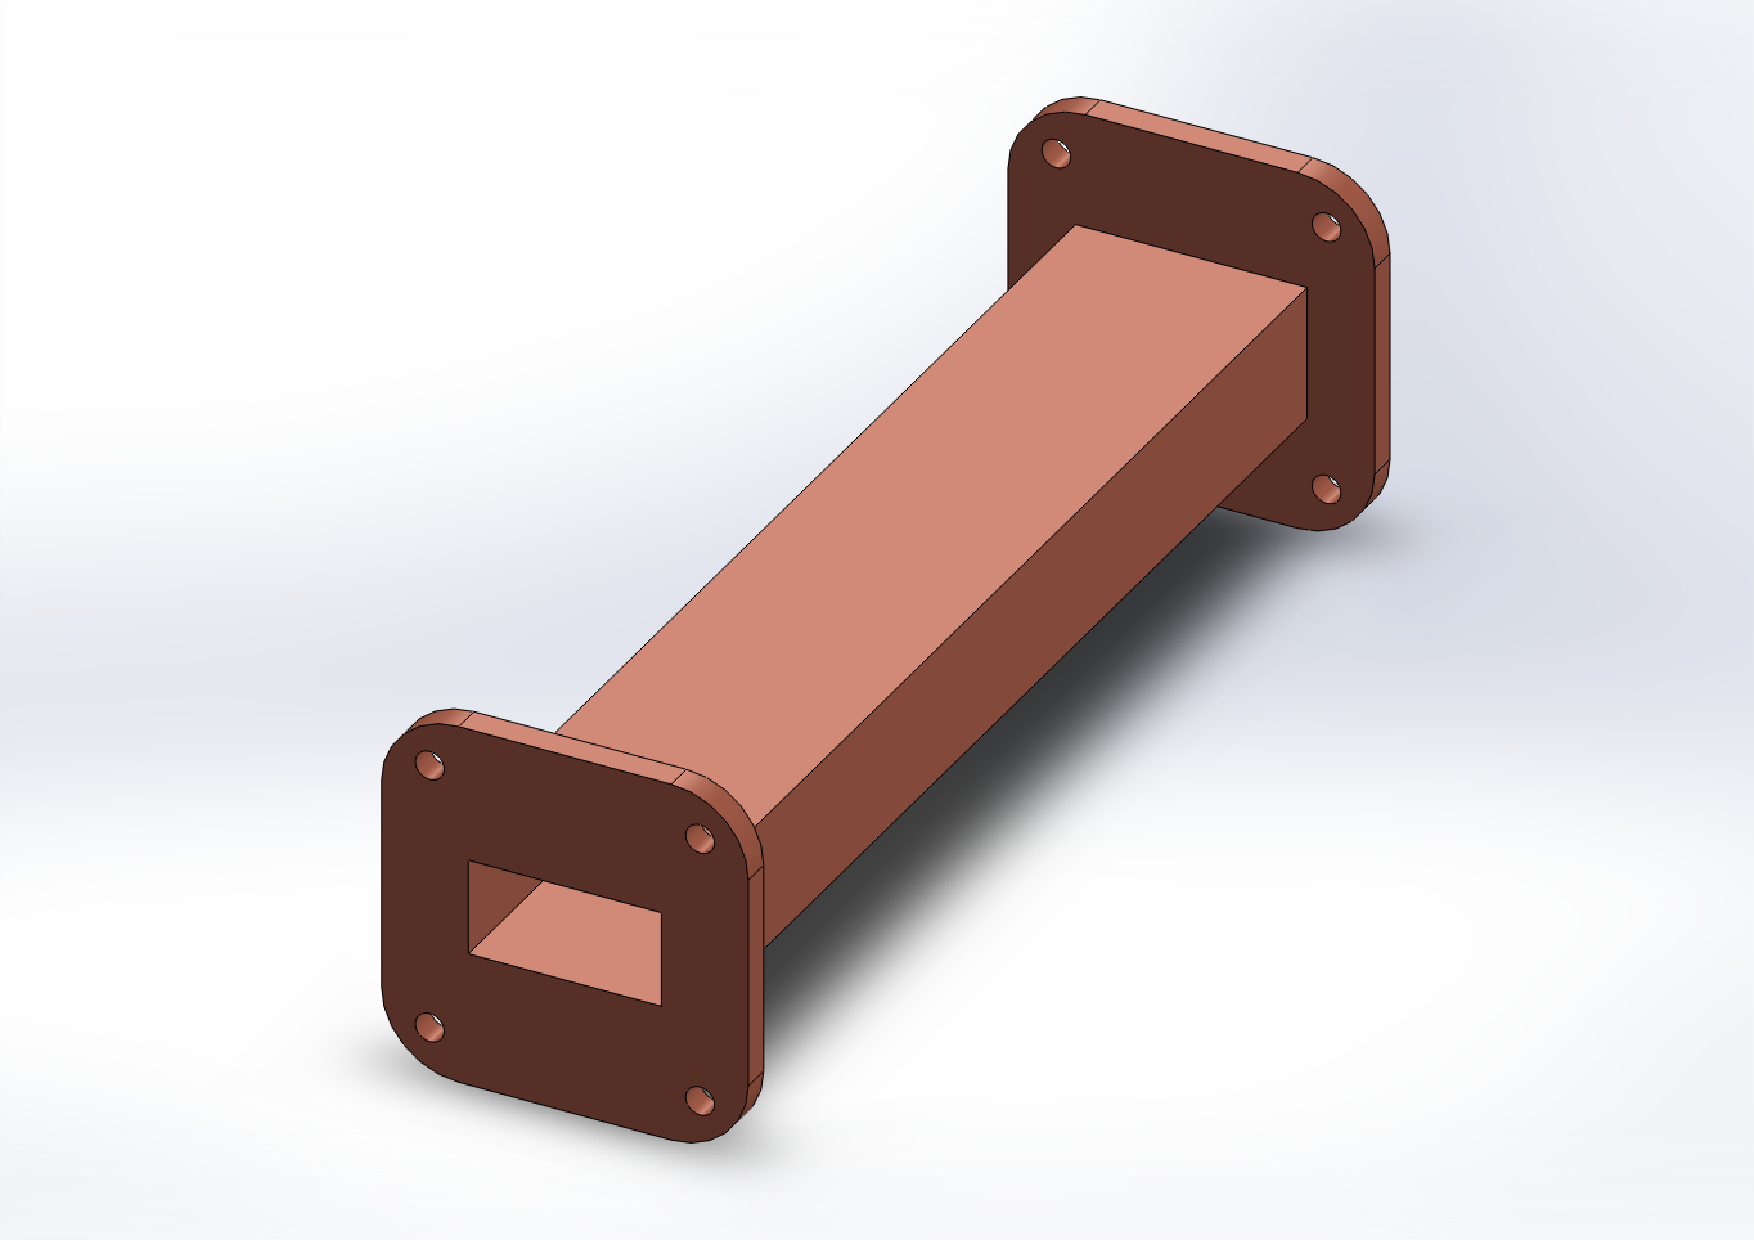
\includegraphics[width=8cm]{vlnovod.pdf}
\caption{Vlnovod masivnější konstrukce pro šíření vln o nižší frekvenci (okolo 1 GHz)}
\label{vlnovod}
\end{center}
\end{figure}

Výhodou vlnovodů je jejich nízký útlum a schopnost přenášet vysoké výkony, stinnou stránkou ale je jejich rozměrnost (čím nižší frekvence, tím masivnější konstrukce) a cena. Pro frekvenci kolem 1 GHz jsou rozměry již 20 cm x 10 cm a s klesající frekvencí dále rostou (viz. obr. \ref{vlnovod}. Pro vysoké frekvence (nad 100 GHz) naopak rozměry klesají na desetiny milimetru a takovéto vlnovody jsou proto náročné na výrobu. Nezřídka se proto používají tzv. nadrozměrné vlnovody, kdy velikost vlnovodu překročí hranici pro šíření jednoho vidu a vlnovodem se šíří vidů více. 
%Možno doplnit: "Pro dané rozměry a materiálové vlastnosti vlnovodu se tato hraniční frekvence pro šíření jednoho vidu nazývá frevencí mezní (cutoff) a bude o ní řeč později"

Druhým způsobem pro přenos vysokých frekvencí jsou koaxiální vedení. Koaxiální vedení vynikají šířkou pásma, kterou mohou přenášet a jsou i cenově dostupnější, nicméně již méně jsou vhodná pro stavbu komplexních mikrovlnných komponent.

Alternativu představují planární vlnovody vyráběné ve formě stripline, microstrip, koplanárního vlnovodu a mnoha dalších. Kromě malých rozměrů a nízké ceny umožňují díky planární technologii výroby i snadnou integrovatelnost s dalšími elektronickými prvky a stavbu mikrovlnných obvodů.

Microstrip je dnes nejpoužívanějším médiem pro integrované mikrovlnné obvody. Sestává se z vodivého proužkou, který je od země oddělen dielektrickým substrátem, jak je znázorněno na obr. \ref{microstrip}. Microstrip byl vyvinut v laboratořích ITT jako konkurent jiné technologii, zveřejněné v roce 1952, stripline. Nevýhodou technologie microstrip v porovnání s klasickými vlnovody jsou její vyšší ztráty a nižší výkon, který je schopna přenášet. Z důvodu neuzavřenosti je také microstrip náchylnější na přeslechy a rušení.

\begin{figure}[h] 
\begin{center}
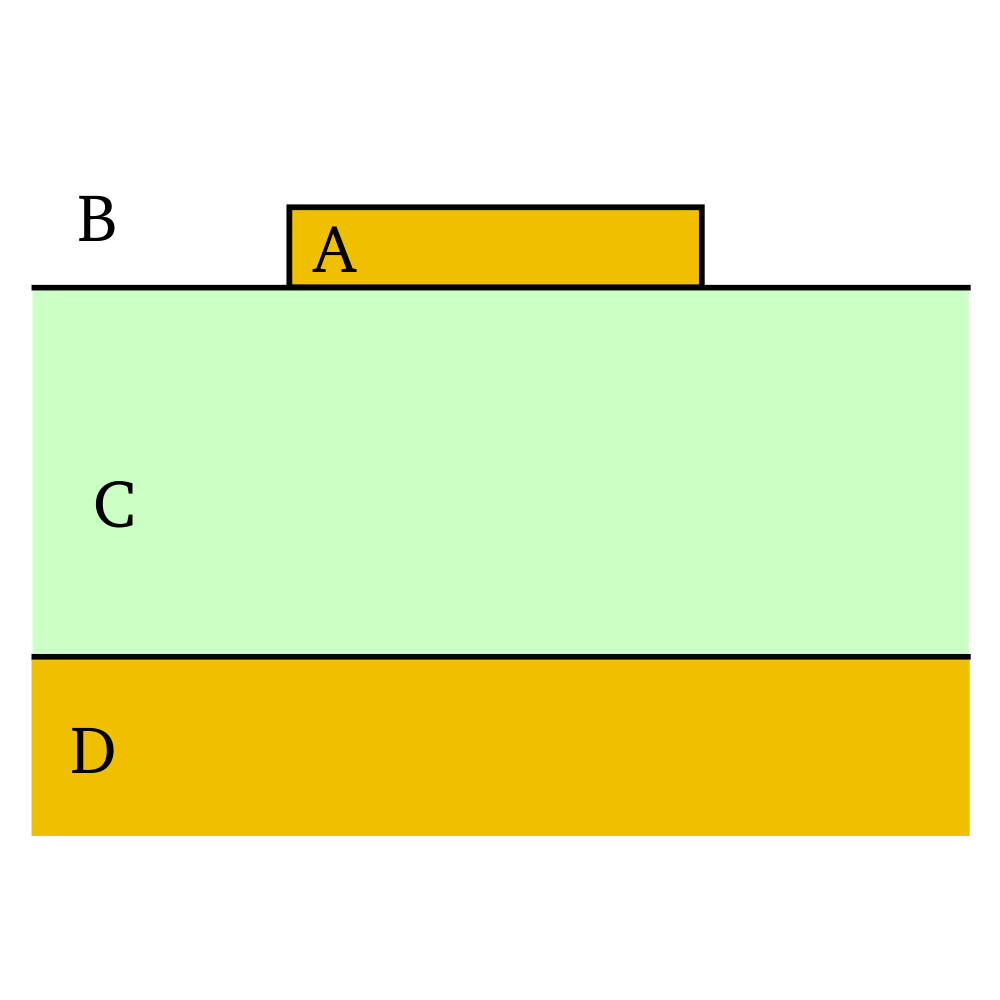
\includegraphics[width=5cm]{microstrip.png}
\caption{Microstrip a jeho části}
\label{microstrip}
\end{center}
\end{figure}

Elektromagnetická vlna šířící se microstripem existuje z části v dielektrickém substrátu a z části ve vzduchu nad ním. A jelikož dielektrická konstanta substrátu je jiná (větší) než vzduchu, vzniká nehomogenní médium, skrz které se vlna šíří. Nehomogenita a frekvenční rozptyl se ještě dále zhoršují spolu s větší šířkou substrátu. Proto až zvládnutí technologie výroby dostatečně tenkých substrátů umožňující menší frekvenční závislost vedení a potlačení podélných složek elektromagnetického pole umožnilo široké rozšíření a skutečný nástup technologie microstrip.
%Možno doplnit: Microstrip neumožňuje šíření skutečných TEM vln. Při nenulové frekvenci jsou vždy přítomné i podélné složky $\vec{E}$ a $\vec{H}$ pole. Tyto složky jsou ale zanedbatelně malé, proto lze o přítomném poli hovořit jako o kvazi-TEM.

\subsubsection{Typy vln šířících se prostřednictvím vlnovodů}
Za běžných okolností nabývají vektory $\vec{E}$ a $\vec{H}$ hodnot v osách roviny kolmé na šíření pole i roviny rovnoběžné s šířením pole (podélné). V určitých případech však může dojít k potlačení podélné složky šíření. Přenosová vedení skládající se ze dvou a více vodičů umožňují šíření tzv. TEM vln (Transverse ElectroMagnetic - transverzálně elektromagnetických). Tyto vlny postrádají podélnou složku elektrického i magnetického pole. Vlnovody sestávající se z jednoho vodiče umožňují šíření TE vln (Transverse Electric - transverzálně elektrických) postrádajících podélnou složku elektrického pole nebo TM vln (Transverse magnetic - transverzálně magnetických) postrádajících podélnou složku magnetického pole. Nikoli však obou současně. Výhodou TEM vln je, že mají jedinečně definované napětí, proud a charakteristickou impedanci. U TE a TM vln toto jednoznačné určení charakteristické impedance není možné, ale existuje matematický postup, který dokáže úspěšně pracovat s modelem charakteristické impedance i u těchto vln.

\begin{figure} 
\begin{center}
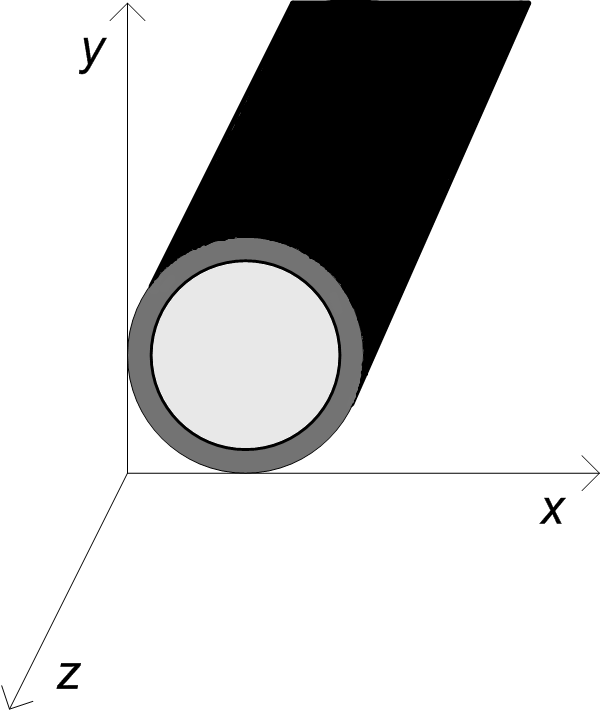
\includegraphics{geometrie.png}
\caption{Geometrie válcového vlnovodu v kartézském souřadném systému}
\label{geometrie}
\end{center}
\end{figure}

\subsubsection{Maxwellovy rovnice pro šíření uvnitř válcových vlnovodů}
Předpokladem je šíření harmonického pole se závislostí $\me ^{jwt}$ podél osy $z$ válcového přenosového vedení nebo vlnovodu, které je ve směru osy $z$ uniformní, nekonečně dlouhé a dokonale vodivé. Geometrie takového vlnovodu je znázorněna na obr. \ref{geometrie} Elektrické a magnetické pole potom může být vyjádřeno takto:
\begin{subequations}
\label{hromadna}
\begin{align}
\faz{\vec{E}}(x, y, z)&=[\faz{\vec{e}}(x, y) + \hat{z}e_z(x, y)] \me ^{j\beta z} ,
\\
\faz{\vec{H}}(x, y, z)&=[\faz{\vec{h}}(x, y) + \hat{z}h_z(x, y)] \me ^{j\beta z} .
\end{align}
\end{subequations}
$\faz{\vec{e}}(x,y)$ a $\faz{\vec{h}}(x,y)$ vyjadřují příčnou (transverzální) složku elektrického a magnetického pole, $e_z$ a $h_z$ představují složku podélnou. Pokud by se vlna šířila v opačném směru (ne ve směru $+z$, ale $-z$), nahradí se $\beta$ za $-\beta$. V případě, kdy by byl přítomen útlum, nahradí se se konstanta šíření $j \beta$ za komplexní konstantu $\gamma$, $\gamma = \alpha + j \beta$.

Pokud ve vlnovodu nebo přenosovém vedení nejsou zdroje $J$, mohou být Maxwellovy rovnice vyjádřeny:
\begin{subequations}
\label{maxvektor2}
\begin{align}
\nabla \times \faz{E} &= -j\omega \mu \faz{H} ,
\\
\nabla \times \faz{H} &= j\omega \varepsilon \faz{E} .
\end{align}
\end{subequations}
.
Tyto vektorové rovnice mohou být převedeny do tvaru jednotlivých parciálních diferenciálních rovnic:
\begin{subequations}
\begin{align}
\frac{\partial E_z}{\partial y} + j \beta E_y &= -j \omega \mu H_x ,
\label{maxpart1}
\\
-j \beta E_x - \frac{\partial E_z}{\partial x} &= - j \omega \mu H_y ,
\\
\frac{\partial E_y}{\partial x} - \frac{\partial E_x}{\partial y} &= -j \omega \mu H_z ,
\end{align}
\end{subequations}
\begin{subequations}
\begin{align}
\frac{\partial H_z}{\partial y} + j \beta H_y &= j \omega \varepsilon E_x ,
\label{maxpart4}
\\
-j \beta H_x - \frac{\partial H_z}{\partial x} &= j \omega \varepsilon E_y ,
\label{maxpart5}
\\
\frac{\partial H_y}{\partial x} - \frac{\partial H_x}{\partial y} &= j \omega \varepsilon E_z .
\end{align}
\end{subequations}

Z těchto rovnic mohou být následně vyjádřeny příčné (transverzální) složky jednotlivých $E$ a $H$ polí:
\begin{subequations}
\label{vyjadreno}
\begin{align}
H_x &= \frac{j}{k^2_c} \left( \omega \varepsilon \frac{\partial E_z}{\partial y} - \beta \frac{\partial H_z}{\partial x} \right) ,
\\
H_y &= \frac{-j}{k^2_c} \left( \omega \varepsilon \frac{\partial E_z}{\partial x} + \beta \frac{\partial H_z}{\partial y} \right) ,
\\
E_x &= \frac{-j}{k^2_c} \left( \beta \frac{\partial E_z}{\partial x} + \omega \mu \frac{\partial H_z}{\partial y} \right) ,
\\
E_y &= \frac{j}{k^2_c} \left(- \beta \frac{\partial E_z}{\partial y} + \omega \mu \frac{\partial H_z}{\partial x} \right) .
\end{align}
\end{subequations}

Příklad výpočtu pro získání složky $H_x$ dosazením $E_y$ z \ref{maxpart5} do \ref{maxpart1}:
%\begin{subequations}
%momentálně uděláno jako nečíslované (pro výpočty)
\begin{align*}
%dále uvažuji, zda centrovat "=" nebo ne
%1. řádek (a)
E_y &= - \frac{\beta H_x}{\omega \varepsilon} - \frac{1}{j \omega \varepsilon} \frac{\partial H_z}{\partial x}
\\
%2. řádek (b)
\frac{\partial E_z}{\partial y} + j \beta \left( - \frac{\beta H_x}{\omega \varepsilon} - \frac{1}{j \omega \varepsilon} \frac{\partial H_z}{\partial x} \right) &= -j \omega \mu H_x
\\
%3. řádek (c)
\frac{\partial E_z}{\partial y} - j \frac{\beta ^2 H_x}{\omega \varepsilon} - \frac{\beta}{\omega \varepsilon} \frac{\partial H_z}{\partial x} &= -j \omega \mu H_x
\\
%4. řádek (d)
\frac{\partial E_z}{\partial y} - \frac{\beta}{\omega \varepsilon} \frac{\partial H_z}{\partial x} &= -j \omega \mu H_x + j \frac{\beta ^2 H_x}{\omega \varepsilon}
\\
%5. řádek (e)
H_x &= \frac{\dfrac{\partial E_z}{\partial y} - \dfrac{\beta ^2}{\omega \varepsilon} \dfrac{\partial H_z}{\partial x}}{-j \omega \mu + j \dfrac{\beta ^2}{\omega \varepsilon}}
\\
%6. řádek (f)
H_x &= j \frac{\dfrac{\partial E_z}{\partial y} - \dfrac{\beta ^2}{\omega \varepsilon} \dfrac{\partial H_z}{\partial x}}{\dfrac{\omega ^2 \varepsilon \mu - \beta ^2}{\omega \varepsilon}}
\\
%7. řádek (g)
H_x &= j \left( \frac{\partial E_z}{\partial y} - \frac{\beta}{\omega \varepsilon} \frac{\partial H_z}{\partial x} \right) \frac{\omega \varepsilon}{\omega ^2 \varepsilon \mu - \beta ^2}
\\
%8. řádek (h)
k^2_c &= k^2 - \beta ^2 = {(\omega \sqrt{\mu \varepsilon})}^2 - \beta ^2 = \omega ^2 \mu \varepsilon - \beta ^2
\\
%9. řádek (i)
H_x &= \frac{j}{k^2_c} \left( \mu \varepsilon \frac{\partial E_z}{\partial y} - \beta \frac{\partial H_z}{\partial x} \right),
\end{align*}
%\end{subequations}
%nevím, jak správně vyjádřit "cutoff" wavenumber - vlnové číslo ?odříznutí? ?mezní?
$k$ je vlnové číslo materiálu uvnitř přenosového vedení nebo vlnovodu, $k_c$ potom tzv. mezní (cutoff) vlnové číslo. V případě přítomnosti ztrát je $\varepsilon$ nahrazeno komplexním $\varepsilon (1 - j \tan{\gamma})$, kde $\gamma$ představuje ztrátový úhel materiálu.

\subsubsection{TEM vlny}
Pro TEM (transverzálně elektromagnetické) vlny platí, že $E_z = 0$ a $H_z = 0$ (není zde přítomna podélná složka elektrického ani magnetického pole). Dosazením těchto hodnot do \ref{vyjadreno} zjistíme, že $H, E = j (0-0) / k^2_c$ a tedy $H, E = 0 / (k^2_c)$. Příčné složky polí jsou tedy také nulové. Pokud se ovšem $k^2_c = 0$, potom získáváme neurčitý výsledek. To mimo jiné znamená, že mezní (cutoff) vlnové číslo pro TEM vlny $k_c = 0$.

Pokud dosadíme $E_z = 0$ do \ref{maxpart1}, $H_x$ poté do \ref{maxpart5} a $H_z = 0$, získáme:
%\begin{subequations}
%momentálně uděláno jako nečíslované (pro výpočty)
\begin{align*}
j \beta E_y &= -j \omega \mu H_x
\\
H_x &= - \frac{\beta E_y}{\omega \mu}
\\
-j \beta \left( - \frac{\beta E_y}{\omega \mu} \right) &= j \omega \varepsilon E_y
\\
\frac{\beta ^2}{\omega \mu} &= \omega \varepsilon
\\
\beta ^2 &= \omega ^2 \mu \varepsilon
\\
\beta &= \omega \sqrt{\mu \varepsilon} .
\end{align*}
%\end{subequations}


Uvažujeme-li kartézský souřadný systém a šíření vlny ve směru osy $z$, lze homogenní Helmholtzovu rovnici \ref{homohelmholtze} přepsat do tvaru:
\begin{equation}
- \frac{\partial ^2}{\partial x^2} - \frac{\partial ^2}{\partial y^2} - \frac{\partial ^2}{\partial z^2} = k^2 \faz{\vec{E}}
\end{equation}
a poté vyjádřit jednotlivé složky $x$, $y$ a $z$:
\begin{subequations}
\begin{align}
\left( \frac{\partial ^2}{\partial x^2} + \frac{\partial ^2}{\partial y^2} + \frac{\partial ^2}{\partial z^2} + k^2 \right) E_x &= 0 , 
\\
\left( \frac{\partial ^2}{\partial x^2} + \frac{\partial ^2}{\partial y^2} + \frac{\partial ^2}{\partial z^2} + k^2 \right) E_y &= 0 ,
\\
\left( \frac{\partial ^2}{\partial x^2} + \frac{\partial ^2}{\partial y^2} + \frac{\partial ^2}{\partial z^2} + k^2 \right) E_z &= 0 .
\end{align}
\end{subequations}
Její tvar pro $k = 0$ a příčné pole bez přítomnosti složky rovnoběžné se směrem šíření se poté zjednoduší na:
\begin{subequations}
\begin{align}
\left( \frac{\partial ^2}{\partial x^2} + \frac{\partial ^2}{\partial y^2} \right) E_x &= 0 ,
\\
\left( \frac{\partial ^2}{\partial x^2} + \frac{\partial ^2}{\partial y^2} \right) E_y &= 0 .
\end{align}
\end{subequations}

Tyto rovnice potom mohou být přepsány do formy využívající Laplacova operátoru ve dvourozměrném příčném poli (poli kolmém ke směru šíření):
\begin{equation}
\triangle _t \faz{e} (x, y) = 0 .
\end{equation}


Stejný postup lze aplikovat i u příčného magnetického pole a dojít ke stejnému výsledku:
\begin{equation}
\triangle _t \faz{h} (x, y) = 0 .
\end{equation}

%%Sekce na přání Pánka vynechána
%%sekce předkládá podobnost EM pole TEM vlny a statického pole mezi dvěma vodiči na základě čehož vyvozuje vztah pro napětí jako rozdíl potenciálů a pro proud na základě Ampérova zákona

%Z toho plyne, že příčné pole TEM vlny je stejné jako statické pole mezi dvěma vodiči. A v případě elektrostatiky lze elektrické pole vyjádřit jako gradient skalárního potenciálu:
%\begin{equation}
%\faz{e} (x, y) = - \nabla _t \Phi (x, y) .
%\end{equation}
%Aby tato rovnice ale mohla platit, musí být ještě splněna podmínka, že pole musí být nevírové:
%\begin{equation}
%\nabla _t \times \faz{e} = 0 ,
%\end{equation}
%což v tomto případě opravdu platí:
%\begin{equation}
%\nabla _t \times \faz{e} = - j \omega \mu h_z \hat{z} = 0 .
%\end{equation}
%
%I toto pole lze potom tedy vyjádřit jako Laplacovu rovnici:
%\begin{equation}
%\nabla ^2_t \Phi (x,y) = 0 .
%\end{equation}
%
%V elektrostatice lze napětí vyjádřit jako rozdíl dvou potenciálů:
%\begin{equation}
%\label{napeti}
%U_{12} = \phi _1 - \phi _2 = \int ^2_1 \faz{E} \ud \faz{l} .
%\end{equation}
%Proud se poté získá z Ampérova zákona:
%\begin{equation}
%\label{amper}
%I = \oint _C \faz{H} \ud \faz{l}.
%\end{equation}

Vlnová impedance TEM vlny se získá jako podíl příčného elektrického a magnetického pole. První rovnice vychází z \ref{maxpart4} při $\beta = \omega \sqrt{\mu \varepsilon}$:
\begin{subequations}
\label{ztem1}
\begin{align}
Z_{TEM} &= \frac{E_x}{H_y}
\\
j \beta H_y &= j \omega \varepsilon E_x
\\
\frac{\beta}{\omega \varepsilon} &= \frac{E_x}{H_y}
\\
\frac{E_x}{H_y} &= \frac{\omega \sqrt{\mu \varepsilon}}{\omega \varepsilon} = \sqrt{\dfrac{\mu}{\varepsilon}} = \eta .
\end{align}
\end{subequations}
Druhá vychází z \ref{maxpart1}:
\begin{subequations}
\label{ztem2}
\begin{align}
Z_{TEM} &= - \frac{E_y}{H_x}
\\
j \beta E_x &= - j \omega \mu H_y
\\
\frac{E_y}{H_x} &= - \frac{\omega \mu}{\beta}
\\
- \frac{E_y}{H_x} &= \frac{\omega \mu}{\omega \sqrt{\mu \varepsilon}} = \sqrt{\dfrac{\mu}{\varepsilon}} = \eta .
\end{align}
\end{subequations}
Výsledky z \ref{ztem1} a \ref{ztem2} je možno spojit do jedné rovnice:
\begin{equation}
\faz{h} (x, y) = \frac{1}{Z_{TEM}} \hat{z} \times \faz{e} (x, y) .
\end{equation}

Charakteristická impedance $Z_0$ se vypočte jako $U / I$ a lze jí získat z \ref{napeti} a \ref{amper}

\subsubsection{TE vlny}
Na rozdíl od TEM vln, kde jsou podélné složky $H$ i $E$ pole nulové, se u TE vln $H_z  \neq 0$. Pro přítomnost podélné složky magnetického pole se jim také říka $H$-vlny. U TE vln mohou být rovnice \ref{vyjadreno} zjednodušeny na:
\begin{subequations}
\begin{align}
H_x &= \frac{-j \beta}{k^2_c} \frac{\partial H_z}{\partial x} ,
\\
H_y &= \frac{-j \beta}{k^2_c} \frac{\partial H_z}{\partial y} ,
\\
E_x &= \frac{-j \omega \mu}{k^2_c} \frac{\partial H_z}{\partial y} ,
\\
E_y &= \frac{j \omega \mu}{k^2_c} \frac{\partial H_z}{\partial x} .
\end{align}
\end{subequations}

U TE vln neplatí, že $k_c = 0$, a konstanta šíření $\beta$ je funkcí frekvence a geometrie vedení. Nejprve se proto musí spočítat $H_z$ z Helmoholtzovi vlnové rovnice (odvození této rovnice je nastíněno v \ref{homohelmholtzb}):
\begin{equation}
\left( \frac{\partial ^2}{\partial x^2} + \frac{\partial ^2}{\partial y^2} + \frac{\partial ^2}{\partial z^2} + k^2 \right) H_z = 0 .
\end{equation}
Tato rovnice může být pro $H_z(x,y,z) = h_z(x,y)e^{-j \beta z}$ upravena na:
\begin{equation}
\left( \frac{\partial ^2}{\partial x^2} + \frac{\partial ^2}{\partial y^2} + k^2_c \right) h_z = 0 .
\end{equation}
K vyřešení této rovnice musí být tedy známy hraniční podmínky a geometrie konkrétního vlnovodu.

Impedance TE vlny je:
\begin{subequations}
\begin{align}
Z_{TE} &= - \frac{E_y}{H_x}
\\
j \beta E_y &= - j \omega \mu H_x
\\
- \frac{E_y}{H_x} &= \frac{\omega \mu}{\beta} ,
\end{align}
\end{subequations}
z čehož plyne, že $Z_{TE}$ je frekvenčně závislé.

\subsubsection{TM vlny}
TM vlny jsou podobné TE vlnám tím, že je v nich též jedna podélná složka pole přítomna. V tomto případě je to složka $z$ pole $E$. Platí tedy $H_z = 0$, $E_z \neq 0$. Tyto vlny jsou proto také někdy nazývány jako $E$ vlny. Rovnice \ref{vyjadreno} mohou být pro TM vlny vyjádřeny jako:
\begin{subequations}
\begin{align}
H_x &= \frac{j \omega \varepsilon}{k^2_c} \frac{\partial E_z}{\partial y} ,
\\
H_y &= \frac{-j \omega \varepsilon}{k^2_c} \frac{\partial E_z}{\partial x} ,
\\
E_x &= \frac{-j \beta}{k^2_c} \frac{\partial E_z}{\partial x} ,
\\
E_y &= \frac{-j \beta}{k^2_c} \frac{\partial E_z}{\partial y} .
\end{align}
\end{subequations}

Stejně jako u TE vln, neplatí, že $k_c = 0$, a konstanta šíření $\beta$ je funkcí frekvence a geometrie vedení. Nejprve se proto musí spočítat $E_z$ z Helmoholtzovi vlnové rovnice (odvození této rovnice je nastíněno v \ref{homohelmholtze}):
\begin{equation}
\left( \frac{\partial ^2}{\partial x^2} + \frac{\partial ^2}{\partial y^2} + \frac{\partial ^2}{\partial z^2} + k^2 \right) E_z = 0 .
\end{equation}
Tato rovnice může být pro $E_z(x,y,z) = e_z(x,y)e^{-j \beta z}$ upravena na:
\begin{equation}
\left( \frac{\partial ^2}{\partial x^2} + \frac{\partial ^2}{\partial y^2} + k^2_c \right) e_z = 0 .
\end{equation}
K vyřešení této rovnice musí být tedy známy hraniční podmínky a geometrie konkrétního vlnovodu.

Impedance TM vlny je:
\begin{subequations}
\begin{align}
Z_{TM} &= \frac{E_x}{H_y}
\\
j \beta H_y &= j \omega \varepsilon E_x
\\
\frac{E_x}{H_y} &= \frac{\beta}{\omega \varepsilon} ,
\end{align}
\end{subequations}
z čehož plyne, že $Z_{TM}$ je frekvenčně závislé.


\newpage
\section{Numerické řešení elektromagnetického pole}

\subsection{Agros 2D}
Agros2D je multiplatformní aplikací zaměřenou na řešení problémů různých fyzikálních polí (od elektrostatického přes akustické po teplotní). Je založen na knihovně Hermes, psané v jazyce C++, využívající pro výpočty metody hp-FEM. Jedná se o verzi metody konečných prvků (FEM - Finite Element Method) pro řešení parciálních diferenciálních rovnic, která je založena na postupné numerické aproximaci udávané elementem o proměnné velikosti ($h$) a stupněm polynomu ($p$). Úvod do metody FEM poskytuje následující kapitola \ref{FEM}. \cite{hpFEM}

Agros2D je volně šiřitelnou open-source aplikací vyvíjenou pod licencí GNU GPL. Zájemce o tento program může zjistit více informací i si stáhnout poslední verzi na stránkách www.agros2d.org (viz \cite{Agros}). Postup vytvoření geometrie a spuštění modelování je také shrnut v příloze B akademické práce \cite{Koudela}.

Pro ukázku je níže znázorněn výstup programu při modelování čtvercového objektu v TM poli:


\subsection{Metoda konečných prvků}
\label{FEM}

\newpage
\section{Návrh modulu pro VF pole}
Navrhovaný modul pro VF pole je .xml soubor obsahující upravené předpisy a rovnice, potřebné pro výpočet veličin vln ve volném prostoru a vlnovodech. Na základě těchto rovnic potom vlastní engine programu Agros2D, knihovna Hermes2D a algoritmus hp fem, vypočítají potřebné veličiny šířící se vlny v jednotlivých bodech zdiskretizovaného prostředí a vytvoří modelové rozložení elektromagnetického pole.

\subsection{Slabé formulace vlnových rovnice}
Prostředí programu Agros2D předpokládá pouze určité typy a způsoby šíření vln vedoucí k zjednodušení modelové situace. Agros2D simuluje pole v 2D prostoru, v třetím rozměru se předpokládá, že je pole rozloženo rovnoměrně nebo symetricky k zakreslené geometrii. Předpokladem je také šíření harmonického pole. Proto je ideální použití Helmholtzovy rovnice (\ref{HelmholtzEnehomo} - Helmholtzova rovnice pro fázor vektoru $\faz{\vec{E}}$).

U Helmholtzovi rovnici dále předpokládáme rovnoměrné rozložení náboje $\rho$. Z toho plyne, že člen $\grad \! \! (\rho / \varepsilon)$ rovnice \ref{HelmholtzEnehomo} bude roven nule. Pro planární problém budeme předpokládat šíření vln v kartézské souřadnicové soustavě ve směru osy $z$. Pro osově symetrický systém bude předpokladem šíření vln v polární souřadnicové soustavě mající pouze tangenciální složku.

Zavedením těchto zjednodušujících předpokladů se Helmholtzova rovnice \ref{HelmholtzEnehomo} transformuje do tvaru:
\begin{equation}
\label{HelmEasy}
\triangle \faz{E} _{(z)} + \faz{k} ^2 \faz{E} _{(z)} = \mj \omega \mu \faz{J} _{ext} .
\end{equation}

Helmholtzovu rovnici pak lze vyjádřit pomocí takzvané slabé formulace. Označme symbolem $u$ člen $\faz{E} _{(z)}$ a symbolem $f$ pravou stranu $\mj \omega \mu \faz{J} _{ext}$. Rovnici roznásobíme testovací funkcí $v$ a následně jí zintegrujeme po ploše $\Omega$ (oblast na které chceme znát řešení - např. vnitřní region vlnovodu):
\begin{subequations}
\label{Poisson}
\begin{align}
- \triangle u - k ~ u &= f
\\
- \triangle u ~ v - k ~ u ~ v &= f ~ v
\\
- \int _{\Omega} \triangle u ~ v ~ \ud \Omega - \int _{\Omega} k ~ u ~ v ~ \ud \Omega &= \int _{\Omega} f ~ v ~ \ud \Omega .
\end{align}
\end{subequations}
Na výraz následně aplikujeme Greenovu větu pomocí které rozložíme operátor $\triangle$ na skalární součin dvou gradientů ($\grad u = \nabla u$):
\begin{equation}
\label{Green}
- \int _{\Omega} \nabla u \cdot \nabla v ~ \ud \Omega + \int _{\Gamma} \frac{\partial u}{\partial n} ~ v ~ \ud \Gamma - \int _{\Omega} k ~ u ~ v ~ \ud \Omega = \int _{\Omega} f ~ v ~ \ud \Omega .
\end{equation}
Člen $\int _{\Gamma} \frac{\partial u}{\partial n} v \ud \Gamma$ vychází z Greenovi věty a představuje Neumannovu okrajovou podmínku. Ve většině případů je tato podmínka (a proto i tento člen) nulová.

Výpočtem divergencí a jejich skalárním roznásobením potom dojdeme k vyjádření výrazu pomocí parciálních diferenciálních rovnic, které již umí řešit Hermes2D a jsou tak vhodné pro simulaci (níže výpočet levé strany \ref{Green}, na pravé se již nic nemění):
\begin{equation}
\begin{split}
- \int _{\Omega} \nabla u \cdot \nabla v ~ \ud \Omega - \int _{\Omega} k ~ u ~ v ~ \ud \Omega &= - \int _{\Omega} \left( \frac{\partial u}{\partial x} + \frac{\partial u}{\partial y} \right) \cdot \left( \frac{\partial v}{\partial x} + \frac{\partial v}{\partial y} \right) \ud \Omega - \int _{\Omega} k ~ u ~ v ~ \ud \Omega =\\
&= - \int _{\Omega} \left( \frac{\partial u}{\partial x} \cdot \frac{\partial v}{\partial x} + \frac{\partial u}{\partial y} \cdot \frac{\partial v}{\partial y} \right) \ud \Omega - \int _{\Omega} k ~ u ~ v ~ \ud \Omega .
\end{split}
\end{equation}


\subsubsection{Slabá formulace fázoru E v kartézské souřadnicové soustavě}

Vycházejme z rovnice \ref{HelmEasy} - nehomogenní Helmholtzovy rovnice pro $\faz{E}$ po aplikování zjednodušujících předpokladů. Prvním krokem pro vyjádření slabé formy je rozložení rovnice na reálnou a imaginární složku:
\begin{equation}
\triangle (E _{zRe} + \mj E _{zIm}) + (\omega ^2 \varepsilon \mu - \mj \omega \mu \gamma) (E _{zRe} + \mj E _{zIm}) = \mj \omega \mu (J _{extRe} + \mj J _{extIm})
\end{equation}
\begin{equation}
\begin{split}
\triangle E _{zRe} + \mj \triangle E _{zIm} + \omega ^2 \varepsilon \mu E_ {zRe} + \mj \omega ^2 \varepsilon \mu E _{zIm} - \mj \omega \mu \gamma E _{zRe} + \omega \mu \gamma E _{zIm} =\\
=\mj \omega \mu J _{extRe} - \omega \mu J _{extIm} .
\end{split}
\end{equation}
Reálnou částí rovnice je:
\begin{align*}
&R_{e}:
\\
&\triangle E_ {zRe} + \omega ^2 \varepsilon \mu E_ {zRe} + \omega \mu \gamma E _{zIm} = - \omega \mu J _{extIm} .
\numberthis
\end{align*}
Imaginární potom:
\begin{align*}
&I_{m}:
\\
&\triangle E _{zIm} + \omega ^2 \varepsilon \mu E _{zIm} - \omega \mu \gamma E _{zRe} = \omega \mu J _{extRe} .
\numberthis
\end{align*}
Obě části roznásobíme testovací funkcí $v$ a následně je  zintegrujeme po ploše $\Omega$ (oblast na které chceme znát řešení - např. vnitřní region vlnovodu; podobně jako v \ref{Poisson}):
\begin{align*}
&R_e:
\\
&\int _{\Omega} \triangle E _{zRe} ~ v ~ \ud \Omega + \omega ^2 \varepsilon \mu \int _{\Omega} E _{zRe} ~ v ~ \ud \Omega + \omega \mu \gamma \int _{\Omega} E _{zIm} ~ v ~ \ud \Omega = - \omega \mu \int _{\Omega} J _{extIm} ~ v ~ \ud \Omega
\numberthis
\end{align*}
\begin{align*}
&I_m:
\\
&\int _{\Omega} \triangle E _{zIm} ~ v ~ \ud \Omega + \omega ^2 \varepsilon \mu \int _{\Omega} E _{zIm} ~ v ~ \ud \Omega - \omega \mu \gamma \int _{\Omega} E _{zRe} ~ v ~ \ud \Omega = \omega \mu \int _{\Omega} J _{extRe} ~ v ~ \ud \Omega .
\numberthis
\end{align*}
Následně aplikujeme Greenovu větu pomocí které rozložíme operátor $\triangle$ na skalární součin dvou divergencí ($\grad E _{zRe} = \nabla E _{zRe}$) (viz \ref{Green}):
\begin{align*}
&R_e:
\\
&- \int _{\Omega} \nabla E _{zRe} \cdot \nabla v ~ \ud \Omega + \int _{\Gamma} \frac{\partial E _{zRe}}{\partial n} ~ v ~ \ud \Gamma + \omega ^2 \varepsilon \mu \int _{\Omega} E _{zRe} ~ v ~ \ud \Omega + \omega \mu \gamma \int _{\Omega} E _{zIm} ~ v ~ \ud \Omega = 
\\
&= - \omega \mu \int _{\Omega} J _{extIm} ~ v ~ \ud \Omega
\numberthis
\end{align*}
\begin{align*}
&I_m:
\\
&- \int _{\Omega} \nabla E _{zIm} \cdot \nabla v ~ \ud \Omega + \int _{\Gamma} \frac{\partial E _{zIm}}{\partial n} ~ v ~ \ud \Gamma + \omega ^2 \varepsilon \mu \int _{\Omega} E _{zIm} ~ v ~ \ud \Omega - \omega \mu \gamma \int _{\Omega} E _{zRe} ~ v ~ \ud \Omega = 
\\
&= \omega \mu \int _{\Omega} J _{extRe} ~ v ~ \ud \Omega .
\numberthis
\end{align*}
Členy $\int _{\Gamma} \frac{\partial E _{zRe}}{\partial n} ~ v ~ \ud \Gamma$ a $\int _{\Gamma} \frac{\partial E _{zIm}}{\partial n} ~ v ~ \ud \Gamma$ představují Neumannovu okrajovou podmínku. 

Složky intenzity elektrického pole jsou v modulu vyjádřeny obecně, proto se vrátíme k substituci $u = E_z$:
\begin{equation}
\begin{split}
&- \int _{\Omega} \nabla u \cdot \nabla v ~ \ud \Omega + \int _{\Gamma} \frac{\partial u}{\partial n} ~ v ~ \ud \Gamma + \omega ^2 \varepsilon \mu \int _{\Omega} u ~ v ~ \ud \Omega + \omega \mu \gamma \int _{\Omega} u ~ v ~ \ud \Omega =\\
&= - \omega \mu \int _{\Omega} \faz{J} _{ext} ~ v ~ \ud \Omega .
\end{split}
\end{equation}
Výpočtem divergencí a jejich skalárním roznásobením potom dojdeme k vyjádření výrazu pomocí parciálních diferenciálních rovnic:
\begin{align*}
&- \int _{\Omega} \left( \frac{\partial u}{\partial x} \cdot \frac{\partial v}{\partial x} + \frac{\partial u}{\partial y} \cdot \frac{\partial v}{\partial y} \right) \ud \Omega + \int _{\Gamma} \frac{\partial u}{\partial n} ~ v ~ \ud \Gamma + \omega ^2 \varepsilon \mu \int _{\Omega} u ~ v ~ \ud \Omega + \omega \mu \gamma \int _{\Omega} u ~ v ~ \ud \Omega =\\
&= - \omega \mu \int _{\Omega} \faz{J} _{ext} ~ v ~ \ud \Omega .
\numberthis
\end{align*}
Ve výrazu zapisovaném do modulu nebudou přímo vyjádřeny integrály. O jejich výpočet se stará knihovna Hermes, ve které je obsažen programový kód umožňující detekci prvků, na které má být integrace aplikována a její následný výpočet. Celou rovnici také vydělíme $\mu$ (pro vyjádření Neumannovy okrajové podmínky v potřebném tvaru) a $\omega$ rozepíšeme pomocí $f$:
\begin{equation}
\label{EzWeakEpsilon}
- \frac{1}{\mu} \left( \frac{\partial u}{\partial x} \cdot \frac{\partial v}{\partial x} + \frac{\partial u}{\partial y} \cdot \frac{\partial v}{\partial y} \right) + \frac{1}{\mu} \frac{\partial u}{\partial n} ~ v + (2 ~ \pi ~ f) ^2 ~ \varepsilon ~ u ~ v + 2 ~ \pi ~ f ~ \gamma ~ u ~ v = - 2 ~ \pi ~ f ~ \faz{J} _{ext} ~ v .
\end{equation}

Pro účely zápisu rovnic do xml modulu, budou rovnice rozděleny podle stran rovnic (levá strana --> maticový zápis, pravá strana --> vektorový zápis) a imaginárních složek. Člen $1/ \mu ~ \partial u / \partial n ~ v$ představující Neumanovu okrajovou podmínku je vyjádřen v jiné části modulu věnující se povrchovým integrálům.

Člen levé strany reálné části
\begin{subequations}
\begin{gather}
- \frac{1}{\mu} \left( \frac{\partial E _{zRe}}{\partial x} \cdot \frac{\partial v}{\partial x} + \frac{\partial E _{zRe}}{\partial y} \cdot \frac{\partial v}{\partial y} \right) + (2 ~ \pi ~ f) ^2 ~ \varepsilon ~ E _{zRe} ~ v
\\
- \frac{1}{\mu} \left( \frac{\partial u}{\partial x} \cdot \frac{\partial v}{\partial x} + \frac{\partial u}{\partial y} \cdot \frac{\partial v}{\partial y} \right) + (2 ~ \pi ~ f) ^2  ~ \varepsilon ~ u ~ v
\end{gather}
\end{subequations}
bude označen indexy i = 1, j = 1. Indexy udávají polohu v matici. Značení i = 1 reflektuje to, že se jedná o reálnou složku, j = 1 odráží to, že jde o plně reálný člen (nejsou v něm složky vztažené k imaginární části). 

Člen levé strany reálné části
\begin{subequations}
\begin{gather}
2 ~ \pi ~ f ~ \gamma ~ E _{zIm} ~ v
\\
2 ~ \pi ~ f ~ \gamma ~ u ~ v
\end{gather}
\end{subequations}
bude označen indexy i = 1, j = 2. Značení i = 1 reflektuje to, že se jedná o reálnou složku, j = 2 odráží to, že jde o člen závislý na imaginární veličině ($E _{zIm}$).


Člen levé strany imaginární části
\begin{subequations}
\begin{gather}
- \frac{1}{\mu} \left( \frac{\partial E _{zIm}}{\partial x} \cdot \frac{\partial v}{\partial x} + \frac{\partial E _{zIm}}{\partial y} \cdot \frac{\partial v}{\partial y} \right) + (2 ~ \pi ~ f) ^2 ~ \varepsilon ~ E _{zIm} ~ v
\\
- \frac{1}{\mu} \left( \frac{\partial u}{\partial x} \cdot \frac{\partial v}{\partial x} + \frac{\partial u}{\partial y} \cdot \frac{\partial v}{\partial y} \right) + (2 ~ \pi ~ f) ^2 ~ \varepsilon ~ u ~ v
\end{gather}
\end{subequations}
bude označen indexy i = 2, j = 2. Značení i = 2 reflektuje to, že se jedná o imaginární složku, j = 2 odráží to, že jde o plně imaginární člen (nejsou v něm složky vztažené k reálné části). 

Člen levé strany imaginární části
\begin{subequations}
\begin{gather}
- 2 ~ \pi ~ f ~ \gamma ~ E _{zRe} ~ v
\\
- 2 ~ \pi ~ f ~ \gamma ~ u ~ v
\end{gather}
\end{subequations}
bude označen indexy i = 2, j = 1. Značení i = 2 reflektuje to, že se jedná o imaginární složku, j = 1 odráží to, že jde o člen závislý na reálné veličině ($E _{zRe}$).

Člen pravé strany reálné části
\begin{equation}
- 2 ~ \pi ~ f ~ J _{extIm} ~ v
\end{equation}
bude označen indexy i = 2, j = 2. Značení z důvodu přehlednosti zachovává oba indexy i a j, přestože se jedná o jednorozměrný vektor, do kterého jsou členy zanášeny. Proto i = j. Zde jsou indexy rovny 2, protože přestože jde o reálnou část, je zde obsažena imaginární veličina ($J _{extIm}$).

Člen pravé strany imaginární části
\begin{equation}
2 ~ \pi ~ f ~ J _{extRe} ~ v
\end{equation}
bude označen indexy i = 1, j = 1. Zde jsou indexy rovny 1, protože přestože jde o imaginární část, je zde obsažena reálná veličina ($J _{extRe}$).

Přesný XML kód použitý pro zápis výše uvedených rovnic je uveden v Příloze 1 v kapitole \nameref{xmlE}.


\subsubsection{Slabá formulace fázoru H v kartézské souřadnicové soustavě}
Formulace vychází z nehomogenní Helmholtzovy rovnice pro $\faz{\vec{H}}$ (\ref{HelmholtzHnehomo}), na kterou se aplikují stejné zjednodušující předpoklady jako na rovnici pro $\faz{E}$. Levá strana tedy bude, stejně jako v rovnici \ref{HelmEasy}, obsahovat veličinu $\faz{H}$ s pouze $z$ složkou pole. Na pravé straně to mimo jiné znamená, že, vzhledem k přítomnosti pouze $z$ složky původního vektoru, se $\rot \faz{J} _{ext} = \left( - \frac{\partial \faz{J} _{ext(x)}}{\partial y} + \frac{\partial \faz{J} _{ext(y)}}{\partial x} \right) \vec{k}$:
\begin{equation}
\label{HelmEasyH}
\triangle \faz{H} _{(z)} + \faz{k} ^2 \faz{H} _{(z)} = - \left( - \frac{\partial \faz{J} _{ext(x)}}{\partial y} + \frac{\partial \faz{J} _{ext(y)}}{\partial x} \right) .
\end{equation}
Prvním krokem pro vyjádření slabé formy je rozložení rovnice na reálnou a imaginární složku:
\begin{equation}
\begin{split}
\triangle (H _{zRe} + \mj H _{zIm}) + (\omega ^2 \varepsilon \mu - \mj \omega \mu \gamma) (H _{zRe} + \mj H _{zIm}) =\\ 
= \left( \frac{\partial J _{extRe(x)}}{\partial y} - \frac{\partial J _{extRe(y)}}{\partial x} \right) + \mj \left( \frac{\partial J _{extIm(x)}}{\partial y} - \frac{\partial J _{extIm(y)}}{\partial x} \right)
\end{split}
\end{equation}
\begin{equation}
\begin{split}
\triangle H _{zRe} + \mj \triangle H _{zIm} + \omega ^2 \varepsilon \mu H_ {zRe} + \mj \omega ^2 \varepsilon \mu H _{zIm} - \mj \omega \mu \gamma H _{zRe} + \omega \mu \gamma H _{zIm} =\\
= \left( \frac{\partial J _{extRe(x)}}{\partial y} - \frac{\partial J _{extRe(y)}}{\partial x} \right) + \mj \left( \frac{\partial J _{extIm(x)}}{\partial y} - \frac{\partial J _{extIm(y)}}{\partial x} \right) .
\end{split}
\end{equation}
Reálnou částí rovnice je:
\begin{align*}
&R_{e}:
\\
&\triangle H_ {zRe} + \omega ^2 \varepsilon \mu H_ {zRe} + \omega \mu \gamma H _{zIm} = \frac{\partial J _{extRe(x)}}{\partial y} - \frac{\partial J _{extRe(y)}}{\partial x} .
\numberthis
\end{align*}
Imaginární potom:
\begin{align*}
&I_{m}:
\\
&\triangle H _{zIm} + \omega ^2 \varepsilon \mu H _{zIm} - \omega \mu \gamma H _{zRe} = \frac{\partial J _{extIm(x)}}{\partial y} - \frac{\partial J _{extIm(y)}}{\partial x} .
\numberthis
\end{align*}
Obě části roznásobíme testovací funkcí $v$ a následně je  zintegrujeme po ploše $\Omega$ (oblast na které chceme znát řešení - např. vnitřní region vlnovodu; podobně jako v \ref{Poisson}):
\begin{align*}
&R_e:
\\
&\int _{\Omega} \triangle H _{zRe} ~ v ~ \ud \Omega + \omega ^2 \varepsilon \mu \int _{\Omega} H _{zRe} ~ v ~ \ud \Omega + \omega \mu \gamma \int _{\Omega} H _{zIm} ~ v ~ \ud \Omega = 
\\
&= \int _{\Omega} \left( \frac{\partial J _{extRe(x)}}{\partial y} - \frac{\partial J _{extRe(y)}}{\partial x} \right) v ~ \ud \Omega
\numberthis
\end{align*}
\begin{align*}
&I_m:
\\
&\int _{\Omega} \triangle H _{zIm} ~ v ~ \ud \Omega + \omega ^2 \varepsilon \mu \int _{\Omega} H _{zIm} ~ v ~ \ud \Omega - \omega \mu \gamma \int _{\Omega} H _{zRe} ~ v ~ \ud \Omega = 
\\
&= \int _{\Omega} \left(\frac{\partial J _{extIm(x)}}{\partial y} - \frac{\partial J _{extIm(y)}}{\partial x} \right) v ~ \ud \Omega
\numberthis
\end{align*}
Následně aplikujeme Greenovu větu pomocí které rozložíme operátor $\triangle$ na skalární součin dvou gradientů ($\grad H _{zRe} = \nabla H _{zRe}$) (viz \ref{Green}):
\begin{align*}
&R_e:
\\
&- \int _{\Omega} \nabla H _{zRe} \cdot \nabla v ~ \ud \Omega + \int _{\Gamma} \frac{\partial H _{zRe}}{\partial n} ~ v ~ \ud \Gamma + \omega ^2 \varepsilon \mu \int _{\Omega} H _{zRe} ~ v ~ \ud \Omega + \omega \mu \gamma \int _{\Omega} H _{zIm} ~ v ~ \ud \Omega =
\\
&= \int _{\Omega} \left( \frac{\partial J _{extRe(x)}}{\partial y} - \frac{\partial J _{extRe(y)}}{\partial x} \right) v ~ \ud \Omega
\numberthis
\end{align*}
\begin{align*}
&I_m:
\\
&- \int _{\Omega} \nabla H _{zIm} \cdot \nabla v ~ \ud \Omega + \int _{\Gamma} \frac{\partial H _{zIm}}{\partial n} ~ v ~ \ud \Gamma + \omega ^2 \varepsilon \mu \int _{\Omega} H _{zIm} ~ v ~ \ud \Omega - \omega \mu \gamma \int _{\Omega} H _{zRe} ~ v ~ \ud \Omega = 
\\
&= \int _{\Omega} \left( \frac{\partial J _{extIm(x)}}{\partial y} - \frac{\partial J _{extIm(y)}}{\partial x} \right) v ~ \ud \Omega
\numberthis
\end{align*}
Členy $\int _{\Gamma} \frac{\partial H _{zRe}}{\partial n} ~ v ~ \ud \Gamma$ a $\int _{\Gamma} \frac{\partial H _{zIm}}{\partial n} ~ v ~ \ud \Gamma$ představují Neumannovu okrajovou podmínku.

Složky intenzity magnetického pole jsou v modulu vyjádřeny obecně, proto se vrátíme k substituci $u = H_z$:
\begin{equation}
\begin{split}
&- \int _{\Omega} \nabla u \cdot \nabla v ~ \ud \Omega + \int _{\Gamma} \frac{\partial u}{\partial n} ~ v ~ \ud \Gamma + \omega ^2 \varepsilon \mu \int _{\Omega} u ~ v ~ \ud \Omega + \omega \mu \gamma \int _{\Omega} u ~ v ~ \ud \Omega = 
\\
&= \int _{\Omega} \left( \frac{\partial \faz{J} _{ext(x)}}{\partial y} - \frac{\partial \faz{J} _{ext(y)}}{\partial x} \right) v ~ \ud \Omega .
\end{split}
\end{equation}
Výpočtem divergencí a jejich skalárním roznásobením potom dojdeme k vyjádření výrazu pomocí parciálních diferenciálních rovnic:
\begin{equation}
\begin{split}
&- \int _{\Omega} \left( \frac{\partial u}{\partial x} \cdot \frac{\partial v}{\partial x} + \frac{\partial u}{\partial y} \cdot \frac{\partial v}{\partial y} \right) \ud \Omega + \int _{\Gamma} \frac{\partial u}{\partial n} ~ v ~ \ud \Gamma + \omega ^2 \varepsilon \mu \int _{\Omega} u ~ v ~ \ud \Omega + \omega \mu \gamma \int _{\Omega} u ~ v ~ \ud \Omega = 
\\
&= \int _{\Omega} \left( \frac{\partial \faz{J} _{ext(x)}}{\partial y} - \frac{\partial \faz{J} _{ext(y)}}{\partial x} \right) v ~ \ud \Omega .
\end{split}
\end{equation}
Ve výrazu zapisovaném do modulu nebudou přímo vyjádřeny integrály. O jejich výpočet se stará knihovna Hermes, ve které je obsažen programový kód umožňující detekci prvků, na které má být integrace aplikována a její následný výpočet. Celou rovnici také vydělíme $\varepsilon$ (pro vyjádření Neumannovy okrajové podmínky v potřebném tvaru) a $\omega$ rozepíšeme pomocí $f$:
\begin{equation}
\label{HzWeakEpsilon}
\begin{split}
&- \frac{1}{\varepsilon} \left( \frac{\partial u}{\partial x} \cdot \frac{\partial v}{\partial x} + \frac{\partial u}{\partial y} \cdot \frac{\partial v}{\partial y} \right) + \frac{1}{\varepsilon} \frac{\partial u}{\partial n} ~ v + (2 ~ \pi ~ f) ^2 ~ \mu ~ u ~ v + 2 ~ \pi ~ f ~ \frac{1}{\varepsilon} ~ \mu ~ \gamma ~ u ~ v =\\
&= \frac{1}{\varepsilon} \left( \frac{\partial \faz{J} _{ext(x)}}{\partial y} - \frac{\partial \faz{J} _{ext(y)}}{\partial x} \right) v .
\end{split}
\end{equation}

Pro účely zápisu rovnic do xml modulu, budou rovnice rozděleny podle stran rovnic (levá strana --> maticový zápis, pravá strana --> vektorový zápis) a imaginárních složek. Člen $1/ \varepsilon ~ \partial u / \partial n ~ v$ představující Neumanovu okrajovou podmínku je vyjádřen v jiné části modulu věnující se povrchovým integrálům.

Člen levé strany reálné části
\begin{subequations}
\begin{gather}
- \frac{1}{\varepsilon} \left( \frac{\partial H _{zRe}}{\partial x} \cdot \frac{\partial v}{\partial x} + \frac{\partial H _{zRe}}{\partial y} \cdot \frac{\partial v}{\partial y} \right) + (2 ~ \pi ~ f) ^2 ~ \mu ~ H _{zRe} ~ v
\\
- \frac{1}{\varepsilon} \left( \frac{\partial u}{\partial x} \cdot \frac{\partial v}{\partial x} + \frac{\partial u}{\partial y} \cdot \frac{\partial v}{\partial y} \right) + (2 ~ \pi ~ f) ^2 ~ \mu ~ u ~ v
\end{gather}
\end{subequations}
bude označen indexy i = 1, j = 1. Indexy udávají polohu v matici. Značení i = 1 reflektuje to, že se jedná o reálnou složku, j = 1 odráží to, že jde o plně reálný člen (nejsou v něm složky vztažené k imaginární části). 

Člen levé strany reálné části
\begin{subequations}
\begin{gather}
2 ~ \pi ~ f ~ \frac{1}{\varepsilon} ~ \mu ~ \gamma ~ H _{zIm} ~ v
\\
2 ~ \pi ~ f ~ \frac{1}{\varepsilon} ~ \mu ~ \gamma ~ u ~ v
\end{gather}
\end{subequations}
bude označen indexy i = 1, j = 2. Značení i = 1 reflektuje to, že se jedná o reálnou složku, j = 2 odráží to, že jde o člen závislý na imaginární veličině ($H _{zIm}$).


Člen levé strany imaginární části
\begin{subequations}
\begin{gather}
- \frac{1}{\varepsilon} \left( \frac{\partial H _{zIm}}{\partial x} \cdot \frac{\partial v}{\partial x} + \frac{\partial H _{zIm}}{\partial y} \cdot \frac{\partial v}{\partial y} \right) + (2 ~ \pi ~ f) ^2 ~ \mu ~ H _{zIm} ~ v
\\
- \frac{1}{\varepsilon} \left( \frac{\partial u}{\partial x} \cdot \frac{\partial v}{\partial x} + \frac{\partial u}{\partial y} \cdot \frac{\partial v}{\partial y} \right) + (2 ~ \pi ~ f) ^2 ~ \mu ~ u ~ v
\end{gather}
\end{subequations}
bude označen indexy i = 2, j = 2. Značení i = 2 reflektuje to, že se jedná o imaginární složku, j = 2 odráží to, že jde o plně imaginární člen (nejsou v něm složky vztažené k reálné části). 

Člen levé strany imaginární části
\begin{subequations}
\begin{gather}
- 2 ~ \pi ~ f ~ \frac{1}{\varepsilon} ~ \mu ~ \gamma ~ H _{zRe} ~ v
\\
- 2 ~ \pi ~ f ~ \frac{1}{\varepsilon} ~ \mu ~ \gamma ~ u ~ v
\end{gather}
\end{subequations}
bude označen indexy i = 2, j = 1. Značení i = 2 reflektuje to, že se jedná o imaginární složku, j = 1 odráží to, že jde o člen závislý na reálné veličině ($H _{zRe}$).

Člen pravé strany reálné části
\begin{equation}
\frac{1}{\varepsilon} \left( \frac{\partial J _{extRe(x)}}{\partial y} - \frac{\partial J _{extRe(y)}}{\partial x} \right) v
\end{equation}
bude označen indexy i = 1, j = 1. Jde o reálnou část s reálnou veličinou ($J _{extRe}$). Značení z důvodu přehlednosti zachovává oba indexy i a j, přestože se jedná o jednorozměrný vektor, do kterého jsou členy zanášeny. Proto i = j.

Člen pravé strany imaginární části
\begin{equation}
\frac{1}{\varepsilon} \left(\frac{\partial J _{extIm(x)}}{\partial y} - \frac{\partial J _{extIm(y)}}{\partial x} \right)  v
\end{equation}
bude označen indexy i = 2, j = 2. Zde jsou indexy rovny 2, protože jde o imaginární část s imaginární veličinou ($J _{extIm}$).

Přesný XML kód použitý pro zápis výše uvedených rovnic je uveden v Příloze 2 v kapitole \nameref{xmlH}. Pravé strany nebyly v modulu implementovány (byly položeny rovny nule), protože je uvažováno pouze šíření v prostoru bez proudové hustoty.


\subsubsection{Slabá formulace fázoru E ve válcové souřadnicové soustavě}

V trojrozměrné válcové souřadné soustavě je poloha bodu určena vzdáleností od středu $r$, úhlem $\varphi$ a vzdáleností od roviny podstavy $z$. Podobně jako v kartézské souřadné soustavě vycházíme z \ref{HelmEasy} - nehomogenní Helmholtzovy rovnice pro $\faz{E}$ po aplikování zjednodušujících předpokladů. Což v tomto případu znamená, že je přítomna pouze složka $\faz{E} _{\varphi}$. Rovnice \ref{HelmEasy} modifikovaná do válcových souřadnic potom vypadá takto:
\begin{equation}
\triangle \faz{E} _{(\varphi)} + \faz{k} ^2 \faz{E} _{(\varphi)} = \mj \omega \mu \faz{J} _{ext} 
\end{equation}

Podobně jako při řešení v kartézské souřadné soustavě musíme rovnice rozložit na řešení pro reálnou a imaginární složku:
\begin{equation}
\triangle (E _{\varphi Re} + \mj E _{\varphi Im}) + (\omega ^2 \varepsilon \mu - \mj \omega \mu \gamma) (E _{\varphi Re} + \mj E _{\varphi Im}) = \mj \omega \mu (J _{extRe} + \mj J _{extIm})
\end{equation}
\begin{equation}
\begin{split}
\triangle E _{\varphi Re} + \mj \triangle E _{\varphi Im} + \omega ^2 \varepsilon \mu E_ {\varphi Re} + \mj \omega ^2 \varepsilon \mu E _{\varphi Im} - \mj \omega \mu \gamma E _{\varphi Re} + \omega \mu \gamma E _{\varphi Im} =\\
= \mj \omega \mu J _{extRe} - \omega \mu J _{extIm} .
\end{split}
\end{equation}
Reálnou částí rovnice je:
\begin{align*}
&R_{e}:
\\
&\triangle E_ {\varphi Re} + \omega ^2 \varepsilon \mu E_ {\varphi Re} + \omega \mu \gamma E _{\varphi Im} = - \omega \mu J _{extIm} .
\numberthis
\end{align*}
Imaginární potom:
\begin{align*}
&I_{m}:
\\
&\triangle E _{\varphi Im} + \omega ^2 \varepsilon \mu E _{\varphi Im} - \omega \mu \gamma E _{\varphi Re} = \omega \mu J _{extRe} .
\numberthis
\end{align*}
Obě části roznásobíme testovací funkcí $v$ a následně je  zintegrujeme po ploše $\Omega$ (oblast na které chceme znát řešení - např. vnitřní region vlnovodu; podobně jako v \ref{Poisson}). Předtím je ale potřeba ještě si uvědomit jednu věc ohledně numerického výpočtu získaného integrálu. Získaný integrál, přestože se zapisuje zjednodušeně jako $\int _{\Omega} u \ud \Omega$ bude vnitřně numericky vypočítán jako trojitý integrál 
\begin{equation}
\iiint \limits_{\varphi ~ r ~ z} u ~ r ~ \ud \varphi ~ \ud r ~ \ud z . 
\end{equation}
Do integrálu $\int _{\Omega} u ~ \ud \Omega$ je proto nutno zapsat $r$ vznikající v trojitém integrálu jako vyjádření úhlové délky pomocí inkrementu infinitezimální hodnoty $r ~ \ud \varphi$: 
\begin{align*}
&R_e:
\\
&\int _{\Omega} r ~ \triangle E _{\varphi Re} ~ v ~ \ud \Omega + \omega ^2 \varepsilon \mu \int _{\Omega} r ~ E _{\varphi Re} ~ v ~ \ud \Omega +  \omega \mu \gamma \int _{\Omega} r ~ E _{\varphi Im} ~ v ~ \ud \Omega =\\
&= - \omega \mu \int _{\Omega} r ~ J _{extIm} ~ v ~ \ud \Omega
\numberthis
\end{align*}
\begin{align*}
&I_m:
\\
&\int _{\Omega} r ~ \triangle E _{\varphi Im} ~ v ~ \ud \Omega + \omega ^2 \varepsilon \mu \int _{\Omega} r ~ E _{\varphi Im} ~ v ~ \ud \Omega - \omega \mu \gamma \int _{\Omega} r ~ E _{\varphi Re} ~ v ~ \ud \Omega =\\ 
&= \omega \mu \int _{\Omega} r ~ J _{extRe} ~ v ~ \ud \Omega .
\numberthis
\end{align*}
Následně aplikujeme Greenovu větu pomocí které rozložíme operátor $\triangle$ na skalární součin dvou gradientů ($\grad E _{\varphi Re} = \nabla E _{\varphi Re}$) (viz \ref{Green}):
\begin{align*}
&R_e:
\\
&- \int _{\Omega} r ~ \nabla E _{\varphi Re} \cdot \nabla v ~ \ud \Omega + \int _{\Gamma} r ~ \frac{\partial E _{\varphi Re}}{\partial n} ~ v ~ \ud \Gamma + \omega ^2 \varepsilon \mu \int _{\Omega} r ~ E _{\varphi Re} ~ v ~ \ud \Omega +\\
& + \omega \mu \gamma \int _{\Omega} r ~ E _{\varphi Im} ~ v ~ \ud \Omega = - \omega \mu \int _{\Omega} r ~ J _{extIm} ~ v ~ \ud \Omega
\numberthis
\end{align*}
\begin{align*}
&I_m:
\\
&- \int _{\Omega} r ~ \nabla E _{\varphi Im} \cdot \nabla v ~ \ud \Omega + \int _{\Gamma} r ~ \frac{\partial E _{\varphi Im}}{\partial n} ~ v ~ \ud \Gamma + \omega ^2 \varepsilon \mu \int _{\Omega} r ~ E _{\varphi Im} \! ~ v ~ \ud \Omega +\\ 
& - \omega \mu \gamma \int _{\Omega} r ~ E _{\varphi Re} ~ v ~ \ud \Omega = \omega \mu \int _{\Omega} r ~ J _{extRe} ~ v ~ \ud \Omega .
\numberthis
\end{align*}
Členy $\int _{\Gamma} r \frac{\partial E _{\varphi Re}}{\partial n} ~ v ~ \ud \Gamma$ a $\int _{\Gamma} r \frac{\partial E _{\varphi Im}}{\partial n} ~ v ~ \ud \Gamma$ představují Neumannovu okrajovou podmínku.

Složky intenzity elektrického pole jsou v modulu vyjádřeny obecně, proto se vrátíme k substituci $u = E_\varphi$:
\begin{align*}
&- \int _{\Omega} r ~ \nabla u \cdot \nabla v ~ \ud \Omega + \int _{\Gamma} r ~ \frac{\partial u}{\partial n} ~ v ~ \ud \Gamma + \omega ^2 \varepsilon \mu \int _{\Omega} r ~ u ~ v ~ \ud \Omega + \omega \mu \gamma \int _{\Omega} r ~ u ~ v ~ \ud \Omega =\\
&= - \omega \mu \int _{\Omega} r ~ \faz{J} _{ext} ~ v ~ \ud \Omega .
\numberthis
\end{align*}
Výpočtem divergencí a jejich skalárním roznásobením potom dojdeme k vyjádření výrazu pomocí parciálních diferenciálních rovnic:
\begin{equation*}
\begin{split}
&- \int _{\Omega} r \left( \frac{\partial u}{\partial r} \cdot \frac{\partial v}{\partial r} + \frac{\partial u}{\partial z} \cdot \frac{\partial v}{\partial z} \right) \ud \Omega + \int _{\Gamma} r ~ \frac{\partial u}{\partial n} ~ v ~ \ud \Gamma + \omega ^2 \varepsilon \mu \int _{\Omega} r ~ u ~ v ~ \ud \Omega +\\
& + \omega \mu \gamma \int _{\Omega} r ~ u ~ v ~ \ud \Omega = - \omega \mu \int _{\Omega} r ~ \faz{J} _{ext} ~ v ~ \ud \Omega .
\end{split}
\numberthis
\end{equation*}
Ve výrazu zapisovaném do modulu nebudou přímo vyjádřeny integrály. O jejich výpočet se stará knihovna Hermes, ve které je obsažen programový kód umožňující detekci prvků, na které má být integrace aplikována a její následný výpočet. Celou rovnici také vydělíme $\mu$ (pro vyjádření Neumannovy okrajové podmínky v potřebném tvaru) a $\omega$ rozepíšeme pomocí $f$:
\begin{equation}
\label{EphiWeakEpsilon}
- r \frac{1}{\mu} \left( \frac{\partial u}{\partial r} \cdot \frac{\partial v}{\partial r} + \frac{\partial u}{\partial z} \cdot \frac{\partial v}{\partial z} \right) + r \frac{1}{\mu} \frac{\partial u}{\partial n} ~ v + r ~ (2 ~ \pi ~ f) ^2 ~ \varepsilon ~ u ~ v + r ~ 2 ~ \pi ~ f ~ \gamma ~ u ~ v = - r ~ 2 ~ \pi ~ f ~ \faz{J} _{ext} ~ v .
\end{equation}

Pro účely zápisu rovnic do xml modulu, budou rovnice rozděleny podle stran rovnic (levá strana --> maticový zápis, pravá strana --> vektorový zápis) a imaginárních složek. Člen $r ~ 1/ \mu ~ \partial u / \partial n ~ v$ představující Neumanovu okrajovou podmínku je vyjádřen v jiné části modulu věnující se povrchovým integrálům.

Člen levé strany reálné části
\begin{subequations}
\begin{gather}
- r \frac{1}{\mu} \left( \frac{\partial E _{\varphi Re}}{\partial r} \cdot \frac{\partial v}{\partial r} + \frac{\partial E _{\varphi Re}}{\partial z} \cdot \frac{\partial v}{\partial z} \right) + r ~ (2 ~ \pi ~ f) ^2 ~ \varepsilon ~ E _{\varphi Re} ~ v
\\
- r \frac{1}{\mu} \left( \frac{\partial u}{\partial r} \cdot \frac{\partial v}{\partial r} + \frac{\partial u}{\partial z} \cdot \frac{\partial v}{\partial z} \right) + r ~ (2 ~ \pi ~ f) ^2  ~ \varepsilon ~ u ~ v
\end{gather}
\end{subequations}
bude označen indexy i = 1, j = 1. Indexy udávají polohu v matici. Značení i = 1 reflektuje to, že se jedná o reálnou složku, j = 1 odráží to, že jde o plně reálný člen (nejsou v něm složky vztažené k imaginární části). 

Člen levé strany reálné části
\begin{subequations}
\begin{gather}
r ~ 2 ~ \pi ~ f ~ \gamma ~ E _{\varphi Im} ~ v
\\
r ~ 2 ~ \pi ~ f ~ \gamma ~ u ~ v
\end{gather}
\end{subequations}
bude označen indexy i = 1, j = 2. Značení i = 1 reflektuje to, že se jedná o reálnou složku, j = 2 odráží to, že jde o člen závislý na imaginární veličině ($E _{\varphi Im}$).


Člen levé strany imaginární části
\begin{subequations}
\begin{gather}
- r \frac{1}{\mu} \left( \frac{\partial E _{\varphi Im}}{\partial r} \cdot \frac{\partial v}{\partial r} + \frac{\partial E _{\varphi Im}}{\partial z} \cdot \frac{\partial v}{\partial z} \right) + r ~ (2 ~ \pi ~ f) ^2 ~ \varepsilon ~ E _{\varphi Im} ~ v
\\
- r \frac{1}{\mu} \left( \frac{\partial u}{\partial r} \cdot \frac{\partial v}{\partial r} + \frac{\partial u}{\partial z} \cdot \frac{\partial v}{\partial z} \right) + r ~ (2 ~ \pi ~ f) ^2 ~ \varepsilon ~ u ~ v
\end{gather}
\end{subequations}
bude označen indexy i = 2, j = 2. Značení i = 2 reflektuje to, že se jedná o imaginární složku, j = 2 odráží to, že jde o plně imaginární člen (nejsou v něm složky vztažené k reálné části). 

Člen levé strany imaginární části
\begin{subequations}
\begin{gather}
- r ~ 2 ~ \pi ~ f ~ \gamma ~ E _{\varphi Re} ~ v
\\
- r ~ 2 ~ \pi ~ f ~ \gamma ~ u ~ v
\end{gather}
\end{subequations}
bude označen indexy i = 2, j = 1. Značení i = 2 reflektuje to, že se jedná o imaginární složku, j = 1 odráží to, že jde o člen závislý na reálné veličině ($E _{\varphi Re}$).

Člen pravé strany reálné části
\begin{equation}
- r ~ 2 ~ \pi ~ f ~ J _{extIm} ~ v
\end{equation}
bude označen indexy i = 2, j = 2. Značení z důvodu přehlednosti zachovává oba indexy i a j, přestože se jedná o jednorozměrný vektor, do kterého jsou členy zanášeny. Proto i = j. Zde jsou indexy rovny 2, protože přestože jde o reálnou část, je zde obsažena imaginární veličina ($J _{extIm}$).

Člen pravé strany imaginární části
\begin{equation}
r ~ 2 ~ \pi ~ f ~ J _{extRe} ~ v
\end{equation}
bude označen indexy i = 1, j = 1. Zde jsou indexy rovny 1, protože přestože jde o imaginární část, je zde obsažena reálná veličina ($J _{extRe}$).

Přesný XML kód použitý pro zápis výše uvedených rovnic je uveden v Příloze 1 v kapitole \nameref{xmlE}.

%%Polární souřadnicová soustava odovzená přes rotace:
%nebo jinak zapsáno též takto:
%\begin{equation}
%\rot \rot \faz{E} _{(\alpha)} + \faz{k} ^2 \faz{E} _{(\alpha)} = \mj \omega \mu \faz{J} _{ext} .
%\end{equation}
%Provedeme vyjádření operace $\rot \faz{E} _{(\alpha)}$:
%\begin{subequations}
%\begin{align}
%\rot \left( \frac{1}{r} \left|
%\begin{array}{c c c}
%\hat{r} & r\hat{\alpha} & \hat{z} \\
%\frac{\partial}{\partial r} & \frac{\partial}{\partial \alpha} & \frac{\partial}{\partial z} \\
%0 & r\faz{E} _{\alpha} & 0
%\end{array} \right| \right)
%+ \faz{k} ^2 \faz{E} _{(\alpha)} &= \mj \omega \mu \faz{J} _{ext} 
%\\
%\rot \left( \frac{1}{r} \frac{\partial}{\partial r} r \faz{R} _{\alpha} \hat{z} - \frac{1}{r} \frac{\partial}{\partial z} r \faz{E} _{\alpha} \hat{r} \right) + \faz{k} ^2 \faz{E} _{(\alpha)} &= \mj \omega \mu \faz{J} _{ext} .
%\end{align}
%\end{subequations}
%A následně stejným způsobem provedeme druhou operaci rotace:
%\begin{subequations}
%\begin{align*}
%&\frac{1}{r} \left|
%\begin{array}{c c c}
%\hat{r} & r\hat{\alpha} & \hat{z} \\
%\frac{\partial}{\partial r} & \frac{\partial}{\partial \alpha} & \frac{\partial}{\partial z} \\
%- \frac{1}{r} \frac{\partial r \faz{E} _{\alpha}}{\partial z} & 0 & \frac{1}{r} \frac{\partial r \faz{E} _{\alpha}}{\partial r}
%\end{array} \right|
%+ \faz{k} ^2 \faz{E} _{(\alpha)} = \mj \omega \mu \faz{J} _{ext} 
%\numberthis
%\\
%\frac{1}{r} \frac{\partial}{\partial \alpha} \frac{1}{r} \frac{\partial}{\partial r} r \faz{E} _{\alpha} \hat{r} + &\left[ \frac{1}{r} \frac{\partial}{\partial z} \left( - \frac{1}{r} \frac{\partial}{\partial z} r \faz{E} _{\alpha} \right) - \frac{1}{r} \frac{\partial}{\partial r} \frac{1}{r} \frac{\partial}{\partial r} \faz{E} _{\alpha} \right] \hat{\alpha} + \frac{1}{r} \frac{\partial}{\partial \alpha} \frac{1}{r} \frac{\partial}{\partial z} r \faz{E} _{\alpha} \hat{z} + \faz{k} ^2 \faz{E} _{(\alpha)} =
%\\
%= \mj \omega \mu \faz{J} _{ext} .
%\numberthis
%\end{align*}
%\end{subequations}


\subsubsection{Slabá formulace fázoru H ve válcové souřadnicové soustavě}

V trojrozměrné válcové souřadné soustavě je poloha bodu určena vzdáleností od středu $r$, úhlem $\varphi$ a vzdáleností od roviny podstavy $z$. Formulace vychází z nehomogenní Helmholtzovy rovnice pro $\faz{\vec{H}}$ (\ref{HelmholtzHnehomo}), na kterou se aplikují stejné zjednodušující předpoklady jako na rovnici pro $\faz{E}$ (\ref{HelmEasy}). Což v tomto případě znamená, že je na levé straně rovnice přítomna pouze složka $\faz{H} _{\varphi}$.Na pravé straně to mimo jiné znamená, že, vzhledem k přítomnosti pouze $\varphi$ složky původního vektoru a aplikaci symetrie, se $\rot \faz{J} _{ext} = \frac{1}{r} \left( \frac{\partial \faz{J} _{ext(r)}}{\partial z} - \frac{\partial \faz{J} _{ext(z)}}{\partial r} \right) \vec{\phi}$. Rovnice \ref{HelmholtzHnehomo} modifikovaná do válcových souřadnic potom vypadá takto:
\begin{equation}
\triangle \faz{H} _{(\varphi)} + \faz{k} ^2 \faz{H} _{(\varphi)} = - \frac{1}{r} \left(  \frac{\partial \faz{J} _{ext(r)}}{\partial z} - \frac{\partial \faz{J} _{ext(z)}}{\partial r} \right)
\end{equation}

Podobně jako při řešení v kartézské souřadné soustavě musíme rovnice rozložit na řešení pro reálnou a imaginární složku:
\begin{equation}
\begin{split}
\triangle (H _{\varphi Re} + \mj H _{\varphi Im}) + (\omega ^2 \varepsilon \mu - \mj \omega \mu \gamma) (H _{\varphi Re} + \mj H _{\varphi Im}) =\\ 
= \frac{1}{r} \left( - \frac{\partial J _{extRe(r)}}{\partial z} + \frac{\partial J _{extRe(z)}}{\partial r} \right) + \mj ~ \frac{1}{r} \left( - \frac{\partial J _{extIm(r)}}{\partial z} + \frac{\partial J _{extIm(z)}}{\partial r} \right)
\end{split}
\end{equation}
\begin{equation}
\begin{split}
\triangle H _{\varphi Re} + \mj \triangle H _{\varphi Im} + \omega ^2 \varepsilon \mu H_ {\varphi Re} + \mj \omega ^2 \varepsilon \mu H _{\varphi Im} - \mj \omega \mu \gamma H _{\varphi Re} + \omega \mu \gamma H _{\varphi Im} =\\
= \frac{1}{r} \left( - \frac{\partial J _{extRe(r)}}{\partial z} + \frac{\partial J _{extRe(z)}}{\partial r} \right) + \mj ~ \frac{1}{r} \left( - \frac{\partial J _{extIm(r)}}{\partial z} + \frac{\partial J _{extIm(z)}}{\partial r} \right) .
\end{split}
\end{equation}
Reálnou částí rovnice je:
\begin{align*}
&R_{e}:
\\
&\triangle H_ {\varphi Re} + \omega ^2 \varepsilon \mu H_ {\varphi Re} + \omega \mu \gamma H _{\varphi Im} = \frac{1}{r} \left( - \frac{\partial J _{extRe(r)}}{\partial z} + \frac{\partial J _{extRe(z)}}{\partial r} \right) .
\numberthis
\end{align*}
Imaginární potom:
\begin{align*}
&I_{m}:
\\
&\triangle H _{\varphi Im} + \omega ^2 \varepsilon \mu H _{\varphi Im} - \omega \mu \gamma H _{\varphi Re} = \frac{1}{r} \left( - \frac{\partial J _{extIm(r)}}{\partial z} + \frac{\partial J _{extIm(z)}}{\partial r} \right) .
\numberthis
\end{align*}
Obě části roznásobíme testovací funkcí $v$ a následně je  zintegrujeme po ploše $\Omega$ (oblast na které chceme znát řešení - např. vnitřní region vlnovodu; podobně jako v \ref{Poisson}). Předtím je ale potřeba ještě si uvědomit jednu věc ohledně numerického výpočtu získaného integrálu. Získaný integrál, přestože se zapisuje zjednodušeně jako $\int _{\Omega} u \ud \Omega$ bude vnitřně numericky vypočítán jako trojitý integrál 
\begin{equation}
\iiint \limits_{\varphi ~ r ~ z} u ~ r ~ \ud \varphi ~ \ud r ~ \ud z . 
\end{equation}
Do integrálu $\int _{\Omega} u ~ \ud \Omega$ je proto nutno zapsat $r$ vznikající v trojitém integrálu jako vyjádření úhlové délky pomocí inkrementu infinitezimální hodnoty $r ~ \ud \varphi$:
\begin{align*}
&R_e:
\\
&\int _{\Omega} r ~ \triangle H _{\varphi Re} ~ v ~ \ud \Omega + \omega ^2 \varepsilon \mu \int _{\Omega} r ~ H _{\varphi Re} ~ v ~ \ud \Omega + \omega \mu \gamma \int _{\Omega} r ~ H _{\varphi Im} ~ v ~ \ud \Omega = 
\\
&= \int _{\Omega} r ~ \frac{1}{r} \left( - \frac{\partial J _{extRe(r)}}{\partial z} + \frac{\partial J _{extRe(z)}}{\partial r} \right) v ~ \ud \Omega
\numberthis
\end{align*}
\begin{align*}
&I_m:
\\
&\int _{\Omega} r ~ \triangle H _{\varphi Im} ~ v ~ \ud \Omega + \omega ^2 \varepsilon \mu \int _{\Omega} r ~ H _{\varphi Im} ~ v ~ \ud \Omega - \omega \mu \gamma \int _{\Omega} r ~ H _{\varphi Re} ~ v ~ \ud \Omega = 
\\
&= \int _{\Omega} r ~ \frac{1}{r} \left( - \frac{\partial J _{extIm(r)}}{\partial z} + \frac{\partial J _{extIm(z)}}{\partial r} \right) v ~ \ud \Omega
\numberthis
\end{align*}
Následně aplikujeme Greenovu větu pomocí které rozložíme operátor $\triangle$ na skalární součin dvou gradientů ($\grad H _{\varphi Re} = \nabla H _{\varphi Re}$) (viz \ref{Green}):
\begin{align*}
&R_e:
\\
&- \int _{\Omega} \! r ~ \nabla H _{\varphi Re} \cdot \nabla v ~ \ud \Omega + \int _{\Gamma} \! r ~ \frac{\partial H _{\varphi Re}}{\partial n} ~ v ~ \ud \Gamma + \omega ^2 \varepsilon \mu \int _{\Omega} \! r ~ H _{\varphi Re} v ~ \ud \Omega +\\
& + \omega \mu \gamma \int _{\Omega} \! r ~ H _{\varphi Im} ~ v ~ \ud \Omega = \int _{\Omega} \left( - \frac{\partial J _{extRe(r)}}{\partial z} + \frac{\partial J _{extRe(z)}}{\partial r} \right) v ~ \ud \Omega
\numberthis
\end{align*}
\begin{align*}
&I_m:
\\
&- \int _{\Omega} \! r ~ \nabla H _{\varphi Im} \cdot \nabla v ~ \ud \Omega + \int _{\Gamma} \! r ~ \frac{\partial H _{\varphi Im}}{\partial n} ~ v ~ \ud \Gamma + \omega ^2 \varepsilon \mu \int _{\Omega} \! r ~ H _{\varphi Im} ~ v ~ \ud \Omega +\\
& - \omega \mu \gamma \int _{\Omega} \! r ~ H _{\varphi Re} ~ v ~ \ud \Omega = \int _{\Omega} \left( - \frac{\partial J _{extIm(r)}}{\partial z} + \frac{\partial J _{extIm(z)}}{\partial r} \right) v ~ \ud \Omega
\numberthis
\end{align*}
Členy $\int _{\Gamma} r ~ \frac{\partial H _{\varphi Re}}{\partial n} ~ v ~ \ud \Gamma$ a $\int _{\Gamma} r ~ \frac{\partial H _{\varphi Im}}{\partial n} ~ v ~ \ud \Gamma$ představují Neumannovu okrajovou podmínku.

Složky intenzity magnetického pole jsou v modulu vyjádřeny obecně, proto se vrátíme k substituci $u = H _{\varphi}$:
\begin{equation}
\begin{split}
&- \int _{\Omega} r ~ \nabla u \cdot \nabla v ~ \ud \Omega + \int _{\Gamma} r ~ \frac{\partial u}{\partial n} ~ v ~ \ud \Gamma + \omega ^2 \varepsilon \mu \int _{\Omega} r ~ u ~ v ~ \ud \Omega + \omega \mu \gamma \int _{\Omega} r ~ u ~ v ~ \ud \Omega = 
\\
&= \int _{\Omega} \left( - \frac{\partial \faz{J} _{ext(r)}}{\partial z} + \frac{\partial \faz{J} _{ext(z)}}{\partial r} \right) v ~ \ud \Omega .
\end{split}
\end{equation}
Výpočtem divergencí a jejich skalárním roznásobením potom dojdeme k vyjádření výrazu pomocí parciálních diferenciálních rovnic:
\begin{align*}
&- \int _{\Omega} r ~ \left( \frac{\partial u}{\partial r} \cdot \frac{\partial v}{\partial r} + \frac{\partial u}{\partial z} \cdot \frac{\partial v}{\partial z} \right) \ud \Omega + \int _{\Gamma} r ~ \frac{\partial u}{\partial n} ~ v ~ \ud \Gamma + \omega ^2 \varepsilon \mu \int _{\Omega} r ~ u ~ v ~ \ud \Omega +\\
& + \omega \mu \gamma \int _{\Omega} r ~ u ~ v ~ \ud \Omega = \int _{\Omega}\left( - \frac{\partial \faz{J} _{ext(r)}}{\partial z} + \frac{\partial \faz{J} _{ext(z)}}{\partial r} \right) v ~ \ud \Omega .
\numberthis
\end{align*}
Ve výrazu zapisovaném do modulu nebudou přímo vyjádřeny integrály. O jejich výpočet se stará knihovna Hermes, ve které je obsažen programový kód umožňující detekci prvků, na které má být integrace aplikována a její následný výpočet. Celou rovnici také vydělíme $\varepsilon$ (pro vyjádření Neumannovy okrajové podmínky v potřebném tvaru) a $\omega$ rozepíšeme pomocí $f$:
\begin{equation}
\label{HphiWeakEpsilon}
\begin{split}
&- r \frac{1}{\varepsilon} \left( \frac{\partial u}{\partial r} \cdot \frac{\partial v}{\partial r} + \frac{\partial u}{\partial z} \cdot \frac{\partial v}{\partial z} \right) + r \frac{1}{\varepsilon} \frac{\partial u}{\partial n} ~ v + r ~ (2 ~ \pi ~ f) ^2 ~ \mu ~ u ~ v + r ~ 2 ~ \pi ~ f ~ \frac{1}{\varepsilon} ~ \mu ~ \gamma ~ u ~ v =\\ 
&= \frac{1}{\varepsilon} \left( - \frac{\partial \faz{J} _{ext(r)}}{\partial z} + \frac{\partial \faz{J} _{ext(z)}}{\partial r} \right) v .
\end{split}
\end{equation}

Pro účely zápisu rovnic do xml modulu, budou rovnice rozděleny podle stran rovnic (levá strana --> maticový zápis, pravá strana --> vektorový zápis) a imaginárních složek. Člen $r ~ 1/ \varepsilon ~ \partial u / \partial n ~ v$ představující Neumanovu okrajovou podmínku je vyjádřen v jiné části modulu věnující se povrchovým integrálům.

Člen levé strany reálné části
\begin{subequations}
\begin{gather}
- r \frac{1}{\varepsilon} \left( \frac{\partial H _{\varphi Re}}{\partial r} \cdot \frac{\partial v}{\partial r} + \frac{\partial H _{\varphi Re}}{\partial z} \cdot \frac{\partial v}{\partial z} \right) + r ~ (2 ~ \pi ~ f) ^2 ~ \mu ~ H _{\varphi Re} ~ v
\\
- r \frac{1}{\varepsilon} \left( \frac{\partial u}{\partial r} \cdot \frac{\partial v}{\partial r} + \frac{\partial u}{\partial z} \cdot \frac{\partial v}{\partial z} \right) + r ~ (2 ~ \pi ~ f) ^2 ~ \mu  ~ u ~ v
\end{gather}
\end{subequations}
bude označen indexy i = 1, j = 1. Indexy udávají polohu v matici. Značení i = 1 reflektuje to, že se jedná o reálnou složku, j = 1 odráží to, že jde o plně reálný člen (nejsou v něm složky vztažené k imaginární části). 

Člen levé strany reálné části
\begin{subequations}
\begin{gather}
r ~ 2 ~ \pi ~ f ~ \frac{1}{\varepsilon} ~ \mu ~ \gamma ~ H _{\varphi Im} ~ v
\\
r ~ 2 ~ \pi ~ f ~ \frac{1}{\varepsilon} ~ \mu ~ \gamma ~ u ~ v
\end{gather}
\end{subequations}
bude označen indexy i = 1, j = 2. Značení i = 1 reflektuje to, že se jedná o reálnou složku, j = 2 odráží to, že jde o člen závislý na imaginární veličině ($H _{\varphi Im}$).


Člen levé strany imaginární části
\begin{subequations}
\begin{gather}
- r \frac{1}{\varepsilon} \left( \frac{\partial H _{\varphi Im}}{\partial r} \cdot \frac{\partial v}{\partial r} + \frac{\partial H _{\varphi Im}}{\partial z} \cdot \frac{\partial v}{\partial z} \right) + r ~ (2 ~ \pi ~ f) ^2 ~ \mu ~ H _{\varphi Im} ~ v
\\
- r \frac{1}{\varepsilon} \left( \frac{\partial u}{\partial r} \cdot \frac{\partial v}{\partial r} + \frac{\partial u}{\partial z} \cdot \frac{\partial v}{\partial z} \right) + r ~ (2 ~ \pi ~ f) ^2 ~ \mu ~ u ~ v
\end{gather}
\end{subequations}
bude označen indexy i = 2, j = 2. Značení i = 2 reflektuje to, že se jedná o imaginární složku, j = 2 odráží to, že jde o plně imaginární člen (nejsou v něm složky vztažené k reálné části). 

Člen levé strany imaginární části
\begin{subequations}
\begin{gather}
- r ~ 2 ~ \pi ~ f ~ \frac{1}{\varepsilon} ~ \mu ~ \gamma ~ H _{\varphi Re} ~ v
\\
- r ~ 2 ~ \pi ~ f ~ \frac{1}{\varepsilon} ~ \mu ~ \gamma ~ u ~ v
\end{gather}
\end{subequations}
bude označen indexy i = 2, j = 1. Značení i = 2 reflektuje to, že se jedná o imaginární složku, j = 1 odráží to, že jde o člen závislý na reálné veličině ($H _{\varphi Re}$).

Člen pravé strany reálné části
\begin{equation}
\frac{1}{\varepsilon} \left( - \frac{\partial J _{extRe(r)}}{\partial z} + \frac{\partial J _{extRe(z)}}{\partial r} \right) v
\end{equation}
bude označen indexy i = 1, j = 1. Jde o reálnou část s reálnou veličinou ($J _{extRe}$). Značení z důvodu přehlednosti zachovává oba indexy i a j, přestože se jedná o jednorozměrný vektor, do kterého jsou členy zanášeny. Proto i = j.

Člen pravé strany imaginární části
\begin{equation}
\frac{1}{\varepsilon} \left( - \frac{\partial J _{extIm(r)}}{\partial z} + \frac{\partial J _{extIm(z)}}{\partial r} \right)  v
\end{equation}
bude označen indexy i = 2, j = 2. Zde jsou indexy rovny 2, protože jde o imaginární část s imaginární veličinou ($J _{extIm}$).

Přesný XML kód použitý pro zápis výše uvedených rovnic je uveden v Příloze 2 v kapitole \nameref{xmlH}. Pravé strany nebyly v modulu implementovány (byly položeny rovny nule), protože je uvažováno pouze šíření v prostoru bez proudové hustoty.


\subsection{Okrajové podmínky}
Okrajové podmínky předepisují chování funkce, nebo derivace funkce, v určitých bodech. Těmito body jsou okraje oblasti, na které danou rovnici řešíme. Při řešení parciálních diferenciálních rovnic vystupují obvykle tři typy okrajových podmínek - Dirichletova okrajová podmínka, Neumannova okrajová podmínka a Newtonova okrajová podmínka.


\subsubsection{Dirichletova okrajová podmínka}
Dirichletova okrajová podmínka vyjadřuje hodnotu funkce $u$ na okraji řešené oblasti. Může být obecně závislá na jednotlivých souřadnicích a na čase: 
\begin{equation}
u = f _{Dir} (x, y, z, t)
\end{equation}

\subsubsection*{Tvar pro $\faz{\vec{E}}$ v kartézských souřadnicích}
Na pravou stranu rovnice náleží veličina pole tj. $\faz{\vec{E}}$. Jedná se o TE vlnu, to znamená, že je přítomna pouze složka $z$ pole $\faz{E}$. Pro zápis do xml modulu je třeba rozložit tuto veličinu na její reálnou složku $E _{(z ~ real)}$ a imaginární složku $E _{(z ~ imag)}$. Reálná složka $E _{(z ~ real)}$ bude označena indexem $i = 1$, imaginární složka $E _{(z ~ imag)}$ indexem $i = 2$. Jedná se o vektorový zápis, zde vystupující jako ,,essential form''.

Přesný XML kód je uveden v Příloze 1 v kapitole \nameref{xmlEs}.

\subsubsection*{Tvar pro $\faz{\vec{H}}$ v kartézských souřadnicích}
Na pravou stranu rovnice náleží veličina pole tj. $\faz{\vec{H}}$. Jedná se o TM vlnu, to znamená, že je přítomna pouze složka $z$ pole $\faz{E}$. Pro zápis do xml modulu je třeba rozložit tuto veličinu na její reálnou složku $H _{(z ~ real}$ a imaginární složku $H _{(z ~ imag)}$. Reálná složka $H _{(z ~ real)}$ bude označena indexem $i = 1$, imaginární složka $H _{(z ~ imag)}$ indexem $i = 2$. Jedná se o vektorový zápis, zde vystupující jako ,,essential form''.

Přesný XML kód je uveden v Příloze 2 v kapitole \nameref{xmlHs}.

\subsubsection*{Tvar pro $\faz{\vec{E}}$ ve válcových souřadnicích}
Na pravou stranu rovnice náleží veličina pole tj. $\faz{\vec{E}}$. Jedná se o TE vlnu, to znamená, že je přítomna pouze složka $\varphi$ pole $\faz{E}$. Pro zápis do xml modulu je třeba rozložit tuto veličinu na její reálnou složku $E _{(\varphi ~ real)}$ a imaginární složku $E _{(\varphi ~ imag)}$. Reálná složka $E _{(\varphi ~ real)}$ bude označena indexem $i = 1$, imaginární složka $E _{(\varphi ~ imag)}$ indexem $i = 2$. Jedná se o vektorový zápis, zde vystupující jako ,,essential form''.

Přesný XML kód je uveden v Příloze 1 v kapitole \nameref{xmlEs}.

\subsubsection*{Tvar pro $\faz{\vec{H}}$ ve válcových souřadnicích}
Na pravou stranu rovnice náleží veličina pole tj. $\faz{\vec{H}}$. Jedná se o TM vlnu, to znamená, že je přítomna pouze složka $\varphi$ pole $\faz{E}$. Pro zápis do xml modulu je třeba rozložit tuto veličinu na její reálnou složku $H _{(\varphi ~ real)}$ a imaginární složku $H _{(\varphi ~ imag)}$. Reálná složka $H _{(\varphi ~ real)}$ bude označena indexem $i = 1$, imaginární složka $H _{(\varphi ~ imag)}$ indexem $i = 2$. Jedná se o vektorový zápis, zde vystupující jako ,,essential form''.

Přesný XML kód je uveden v Příloze 2 v kapitole \nameref{xmlHs}.


\subsubsection{Neumannova okrajová podmínka}
Neumannova okrajová podmínka říká, jak se mění veličina ve směru kolmo na rozhraní. Je vyjádřena jako hodnota normálové derivace funkce. V kartézském souřadném systému ji lze obecně zapsat takto:
\begin{equation}
\frac{\partial u}{\partial \vec{n}} = f _{Neu} (x, y, z, t) .
\end{equation}

\subsubsection*{Tvar pro $\faz{\vec{E}}$ v kartézských souřadnicích}
\label{NeumannEK}
Neumannova okrajová podmínka se objeví při výpočtu slabých forem jako člen integro-diferenciální rovnice (\ref{EzWeakEpsilon}) ve formě plošného integrálu:
\begin{subequations}
\label{weakneumann}
\begin{align}
\frac{1}{\mu} \int _{\Gamma} \frac{\partial E _{z Re}}{\partial \vec{n}} ~ v ~ \ud \Gamma ,
\\ 
\frac{1}{\mu} \int _{\Gamma} \frac{\partial E _{z Im}}{\partial \vec{n}} ~ v ~ \ud \Gamma .
\end{align}
\end{subequations}

Pro získání její hodnoty budeme vycházet z \ref{max2fharm} (2. Maxwellovy rovnice ve frekvenční oblasti pro harmonicky proměnné pole). Na levé straně provedeme výpočet operace rotace. Vzhledem k přítomnosti pouze $z$ složky $E$ u TE vlny dojde k zjednodušení výsledku:
\begin{equation}
\left| 
\begin{array}{c c c}
\vec{i} & \vec{j} & \vec{k} \\ 
\frac{\partial}{\partial x} & \frac{\partial}{\partial y} & \frac{\partial}{\partial z} \\
0 & 0 & \faz{E}_z
\end{array}
\right|
= \frac{\partial \faz{E}_z}{\partial y} ~ \vec{i} - \frac{\partial \faz{E}_z}{\partial x} ~ \vec{j}  .
\end{equation} 
Právě vypočtenou levou, i pravou stranu následně roznásobíme vektorem $\vec{n}$ (vektorem normálovým na rozhraní):
\begin{equation}
\vec{n} \times \left( \frac{\partial \faz{E}_z}{\partial y} ~ \vec{i} - \frac{\partial \faz{E}_z}{\partial x} ~ \vec{j} \right) = - ~ \vec{n} \times \mj \omega \mu \faz{\vec{H}} .
\end{equation}
Vektorový součin na levé straně vyřešíme s pomocí determinantu:
\begin{subequations}
\begin{align}
\left| 
\begin{array}{c c c}
\vec{i} & \vec{j} & \vec{k} \\ 
n_x & n_y & n_z \\
\frac{\partial \faz{E}_z}{\partial y} & - \frac{\partial \faz{E}_z}{\partial x} & 0
\end{array}
\right|
= - ~ \vec{n} \times \mj \omega \mu \faz{\vec{H}} 
\\
\left( - \frac{\partial \faz{E}_z}{\partial y} n_y - \frac{\partial \faz{E}_z}{\partial x} n_x \right) \cdot \vec{k} = - ~ \vec{n} \times \mj \omega \mu \faz{\vec{H}}
\\
\left( \frac{\partial \faz{E}_z}{\partial x} ; \frac{\partial \faz{E}_z}{\partial y} \right) \cdot \left( n_x; n_y \right) \cdot \vec{k} = - ~ \vec{n} \times \mj \omega \mu \faz{\vec{H}} .
\end{align}
\end{subequations}
Výraz na levé straně lze také vyjádřit pomocí gradientu:
\begin{equation}
\grad \faz{E}_z \cdot \vec{n} \cdot \vec{k} = - ~ \vec{n} \times \mj \omega \mu \faz{\vec{H}} .
\end{equation}

A samotná Neumannova okrajová podmínka může být též rozepsána pomocí gradientu:
\begin{equation}
\label{gradneumann}
\frac{\partial \faz{E}_z}{\partial \vec{n}} = grad \faz{E}_z \cdot \vec{n} .
\end{equation}
To znamená, že na levou stranu rovnice \ref{gradneumann} můžeme dosadit výraz představující Neumannovu okrajovou podmínku:
\begin{equation}
\frac{\partial \faz{E}_z}{\partial \vec{n}} \cdot \vec{k} = - ~ \vec{n} \times \mj \omega \mu \faz{\vec{H}}.
\end{equation}
Roznásobíme-li pravou stranu normálovým vektorem $\vec{n}$ (a levou stranu vektorem $\vec{k}$) obsahujícím pouze tečnou složku, dostaneme skalární vyjádření:
\begin{equation}
\label{neumann}
\frac{\partial \faz{E}_z}{\partial \vec{n}} = - \mj \omega \mu \faz{H}_t .
\end{equation}
Na levé straně máme tedy zápis Neumannovy okrajové podmínky a na straně pravé její funkční vyjádření.

Posledním krokem je dosazení pravé strany z \ref{neumann} do \ref{weakneumann} (výrazu získaného při výpočtu slabých norem):
\begin{subequations}
\begin{align}
\frac{1}{\mu} \int _{\Gamma} ( \omega \mu H_{(t~imag)} ~ v ) ~ \ud \Gamma ,
\\ 
\frac{1}{\mu} \int _{\Gamma} ( - \mj \omega \mu H_{(t~real)} ~ v ) ~ \ud \Gamma .
\end{align}
\end{subequations}

Takto získaný výraz lze již (bez integrálu o jehož detekci a výpočet se stará samotný programový kód Agrosu) zapsat do xml modulu. Bude se jednat o vyjádření pravé strany, tudíž ,,vector form''. Člen $\mu$ se vykrátí a $\omega$ rozepíšeme pomocí $f$. Reálná složka 
\begin{equation}
2 ~ \pi ~ f ~ H_{(t~imag)} ~ v
\end{equation} 
bude označena indexy i = 1, j = 1. Imaginární složka 
\begin{equation}
- 2 ~ \pi ~ f ~ H_{(t~real)} ~ v
\end{equation}
bude označena indexy i = 2, j = 2.

Přesný XML kód je uveden v Příloze 1 v kapitole \nameref{xmlEs}.

\subsubsection*{Tvar pro $\faz{\vec{H}}$ v kartézských souřadnicích}
\label{NeumannHK}
Neumannova okrajová podmínka se objeví při výpočtu slabých forem jako člen integro-diferenciální rovnice (\ref{HzWeakEpsilon}) ve formě plošného integrálu:
\begin{subequations}
\label{Hweakneumann}
\begin{align}
\frac{1}{\varepsilon} \int _{\Gamma} \frac{\partial H _{z Re}}{\partial \vec{n}} ~ v ~ \ud \Gamma ,
\\ 
\frac{1}{\varepsilon} \int _{\Gamma} \frac{\partial H _{z Im}}{\partial \vec{n}} ~ v ~ \ud \Gamma .
\end{align}
\end{subequations}

Pro získání její hodnoty budeme vycházet z \ref{max1fharm} (1. Maxwellovy rovnice ve frekvenční oblasti pro harmonicky proměnné pole). Na levé straně provedeme výpočet operace rotace. Vzhledem k přítomnosti pouze $z$ složky $H$ u TM vlny dojde k zjednodušení výsledku:
\begin{equation}
\left| 
\begin{array}{c c c}
\vec{i} & \vec{j} & \vec{k} \\ 
\frac{\partial}{\partial x} & \frac{\partial}{\partial y} & \frac{\partial}{\partial z} \\
0 & 0 & \faz{H}_z
\end{array}
\right|
= \frac{\partial \faz{H}_z}{\partial y} ~ \vec{i} - \frac{\partial \faz{H}_z}{\partial x} ~ \vec{j}  .
\end{equation} 
Právě vypočtenou levou, i pravou stranu následně roznásobíme vektorem $\vec{n}$ (vektorem normálovým na rozhraní):
\begin{equation}
\vec{n} \times \left( \frac{\partial \faz{H}_z}{\partial y} ~ \vec{i} - \frac{\partial \faz{H}_z}{\partial x} ~ \vec{j} \right) = \vec{n} \times \mj \omega \varepsilon \faz{\vec{E}} .
\end{equation}
Vektorový součin na levé straně vyřešíme s pomocí determinantu:
\begin{subequations}
\begin{align}
\left| 
\begin{array}{c c c}
\vec{i} & \vec{j} & \vec{k} \\ 
n_x & n_y & n_z \\
\frac{\partial \faz{H}_z}{\partial y} & - \frac{\partial \faz{H}_z}{\partial x} & 0
\end{array}
\right|
= \vec{n} \times \mj \omega \varepsilon \faz{\vec{E}} 
\\
\left( - \frac{\partial \faz{H}_z}{\partial y} n_y - \frac{\partial \faz{H}_z}{\partial x} n_x \right) \cdot \vec{k} = \vec{n} \times \mj \omega \varepsilon \faz{\vec{E}}
\\
\left( \frac{\partial \faz{H}_z}{\partial x} ; \frac{\partial \faz{H}_z}{\partial y} \right) \cdot \left( n_x; n_y \right) \cdot \vec{k} = \vec{n} \times \mj \omega \varepsilon \faz{\vec{E}} .
\end{align}
\end{subequations}
Výraz na levé straně lze také vyjádřit pomocí gradientu:
\begin{equation}
\grad \faz{H}_z \cdot \vec{n} \cdot \vec{k} = \vec{n} \times \mj \omega \varepsilon \faz{\vec{E}} .
\end{equation}

A samotná Neumannova okrajová podmínka může být též rozepsána pomocí gradientu:
\begin{equation}
\label{Hgradneumann}
\frac{\partial \faz{H}_z}{\partial \vec{n}} = grad \faz{H}_z \cdot \vec{n} .
\end{equation}
To znamená, že na levou stranu rovnice \ref{Hgradneumann} můžeme dosadit výraz představující Neumannovu okrajovou podmínku:
\begin{equation}
\frac{\partial \faz{H}_z}{\partial \vec{n}} \cdot \vec{k} = \vec{n} \times \mj \omega \varepsilon \faz{\vec{E}}.
\end{equation}
Roznásobíme-li pravou stranu normálovým vektorem $\vec{n}$ (a levou stranu vektorem $\vec{k}$) obsahujícím pouze tečnou složku, dostaneme skalární vyjádření:
\begin{equation}
\label{Hneumann}
\frac{\partial \faz{H}_z}{\partial \vec{n}} = \mj \omega \varepsilon \faz{E}_t .
\end{equation}
Na levé straně máme tedy zápis Neumannovy okrajové podmínky a na straně pravé její funkční vyjádření.

Posledním krokem je dosazení pravé strany z \ref{Hneumann} do \ref{Hweakneumann} (výrazu získaného při výpočtu slabých norem):
\begin{subequations}
\begin{align}
\frac{1}{\varepsilon} \int _{\Gamma} (- \omega \varepsilon E_{(t~imag)} ~ v ) ~ \ud \Gamma ,
\\ 
\frac{1}{\varepsilon} \int _{\Gamma} (\mj \omega \varepsilon E_{(t~real)} ~ v ) ~ \ud \Gamma .
\end{align}
\end{subequations}

Takto získaný výraz lze již (bez integrálu o jehož detekci a výpočet se stará samotný programový kód Agrosu) zapsat do xml modulu. Bude se jednat o vyjádření pravé strany, tudíž ,,vector form''. Člen $\varepsilon$ se vykrátí a $\omega$ rozepíšeme pomocí $f$. Reálná složka  
\begin{equation}
- 2 ~ \pi ~ f ~ E_{(t~imag)} ~ v
\end{equation} 
bude označena indexy i = 1, j = 1. Imaginární složka 
\begin{equation}
2 ~ \pi ~ f ~ E_{(t~real)} ~ v
\end{equation}
bude označena indexy i = 2, j = 2.

Přesný XML kód je uveden v Příloze 2 v kapitole \nameref{xmlHs}.

\subsubsection*{Tvar pro $\faz{\vec{E}}$ ve válcových souřadnicích}
\label{NeumannEC}
Neumannova okrajová podmínka se objeví při výpočtu slabých forem jako člen integro-diferenciální rovnice (\ref{EphiWeakEpsilon}) ve formě plošného integrálu:
\begin{subequations}
\label{ECweakneumann}
\begin{align}
\frac{1}{\mu} \int _{\Gamma} r ~ \frac{\partial E _{\varphi Re}}{\partial \vec{n}} ~ v ~ \ud \Gamma ,
\\ 
\frac{1}{\mu} \int _{\Gamma} r ~ \frac{\partial E _{\varphi Im}}{\partial \vec{n}} ~ v ~ \ud \Gamma .
\end{align}
\end{subequations}

Pro získání její hodnoty budeme vycházet z \ref{max2fharm} (2. Maxwellovy rovnice ve frekvenční oblasti pro harmonicky proměnné pole). Na levé straně provedeme výpočet operace rotace. Vzhledem k přítomnosti pouze $\varphi$ složky $E$ u TE vlny dojde k zjednodušení výsledku:
\begin{equation}
\rot \! \faz{\vec{E}} = - \frac{\partial \faz{E} _{\varphi}}{\partial z} ~ \vec{\rho} + \frac{1}{r} \frac{\partial ( r \faz{E} _{\varphi} ) }{\partial r} ~ \vec{k} .
\end{equation}
Právě vypočtenou levou, i pravou stranu následně roznásobíme vektorem $\vec{n}$ (vektorem normálovým na rozhraní):
\begin{equation}
\vec{n} \times \left( \frac{1}{r} \frac{\partial ( r \faz{E} _{\varphi} ) }{\partial r} ~ \vec{k} - \frac{\partial \faz{E}_{\varphi}}{\partial z} ~ \vec{\rho} \right) = - ~ \vec{n} \times \mj \omega \mu \faz{\vec{H}} .
\end{equation}
Vektorový součin na levé straně vyřešíme s pomocí determinantu:
\begin{subequations}
\begin{align}
\left| 
\begin{array}{c c c}
\vec{\rho} & \vec{\phi} & \vec{k} \\ 
n_r & n_{\varphi} & n_z \\
\frac{1}{r} \frac{\partial ( r \faz{E} _{\varphi} ) }{\partial r} & 0 & - \frac{\partial \faz{E} _{\varphi}}{\partial z}
\end{array}
\right|
= - ~ \vec{n} \times \mj \omega \mu \faz{\vec{H}} 
\\
\left( \frac{\partial \faz{E}_{\varphi}}{\partial z} n_{r} + \frac{1}{r} \frac{\partial ( r \faz{E} _{\varphi} ) }{\partial r} n_z \right) \cdot \vec{\phi} = - ~ \vec{n} \times \mj \omega \mu \faz{\vec{H}}
\\
\left( \frac{\partial \faz{E} _{\varphi}}{\partial z} ;\frac{1}{r} \frac{\partial ( r \faz{E} _{\varphi} ) }{\partial r} \right) \cdot \left( n_r; n_{z} \right) \cdot \vec{\phi} = - ~ \vec{n} \times \mj \omega \mu \faz{\vec{H}} .
\end{align}
\end{subequations}
Výraz na levé straně lze také vyjádřit pomocí gradientu:
\begin{equation}
\grad \faz{E} _{\varphi} \cdot \vec{n} \cdot \vec{\phi} = - ~ \vec{n} \times \mj \omega \mu \faz{\vec{H}} .
\end{equation}

A samotná Neumannova okrajová podmínka může být též rozepsána pomocí gradientu:
\begin{equation}
\label{ECgradneumann}
\frac{\partial \faz{E} _{\varphi}}{\partial \vec{n}} = grad \faz{E} _{\varphi} \cdot \vec{n} .
\end{equation}
To znamená, že na levou stranu rovnice \ref{ECgradneumann} můžeme dosadit výraz představující Neumannovu okrajovou podmínku:
\begin{equation}
\frac{\partial \faz{E}_{\varphi}}{\partial \vec{n}} \cdot \vec{\phi} = - ~ \vec{n} \times \mj \omega \mu \faz{\vec{H}} .
\end{equation}
Roznásobíme-li pravou stranu normálovým vektorem $\vec{n}$ (a levou stranu vektorem $\vec{\phi}$) obsahujícím pouze tečnou složku, dostaneme skalární vyjádření:
\begin{equation}
\label{ECneumann}
\frac{\partial \faz{E}_{\varphi}}{\partial \vec{n}} = - \mj \omega \mu \faz{H}_t .
\end{equation}
Na levé straně máme tedy zápis Neumannovy okrajové podmínky a na straně pravé její funkční vyjádření.

Posledním krokem je dosazení pravé strany z \ref{ECneumann} do \ref{ECweakneumann} (výrazu získaného při výpočtu slabých norem):
\begin{subequations}
\begin{align}
\frac{1}{\mu} \int _{\Gamma} ( \omega \mu H_{(t~imag)} ~ v ) ~ r ~ \ud \Gamma ,
\\ 
\frac{1}{\mu} \int _{\Gamma} ( - \mj \omega \mu H_{(t~real)} ~ v ) ~ r ~ \ud \Gamma .
\end{align}
\end{subequations}

Takto získaný výraz lze již (bez integrálu o jehož detekci a výpočet se stará samotný programový kód Agrosu) zapsat do xml modulu. Bude se jednat o vyjádření pravé strany, tudíž ,,vector form''. Člen $\mu$ se vykrátí a $\omega$ rozepíšeme pomocí $f$. Reálná složka 
\begin{equation}
2 ~ \pi ~ f ~ H_{(t~imag)} ~ r ~ v
\end{equation} 
bude označena indexy i = 1, j = 1. Imaginární složka 
\begin{equation}
- 2 ~ \pi ~ f ~ H_{(t~real)} ~ r ~ v
\end{equation}
bude označena indexy i = 2, j = 2.

Přesný XML kód je uveden v Příloze 1 v kapitole \nameref{xmlEs}.

\subsubsection*{Tvar pro $\faz{\vec{H}}$ ve válcových souřadnicích}
\label{NeumannHC}
Neumannova okrajová podmínka se objeví při výpočtu slabých forem jako člen integro-diferenciální rovnice (\ref{HphiWeakEpsilon}) ve formě plošného integrálu:
\begin{subequations}
\label{HCweakneumann}
\begin{align}
\frac{1}{\varepsilon} \int _{\Gamma} r ~ \frac{\partial H _{\varphi Re}}{\partial \vec{n}} ~ v ~ \ud \Gamma ,
\\ 
\frac{1}{\varepsilon} \int _{\Gamma} r ~ \frac{\partial H _{\varphi Im}}{\partial \vec{n}} ~ v ~ \ud \Gamma .
\end{align}
\end{subequations}

Pro získání její hodnoty budeme vycházet z \ref{max1fharm} (1. Maxwellovy rovnice ve frekvenční oblasti pro harmonicky proměnné pole). Na levé straně provedeme výpočet operace rotace. Vzhledem k přítomnosti pouze $\varphi$ složky $H$ u TM vlny dojde k zjednodušení výsledku:
\begin{equation}
\rot \! \faz{\vec{H}} = - \frac{\partial \faz{H} _{\varphi}}{\partial z} ~ \vec{\rho} + \frac{1}{r} \frac{\partial ( r \faz{H} _{\varphi} ) }{\partial r} ~ \vec{k} .
\end{equation}
Právě vypočtenou levou, i pravou stranu následně roznásobíme vektorem $\vec{n}$ (vektorem normálovým na rozhraní):
\begin{equation}
\vec{n} \times \left( \frac{1}{r} \frac{\partial ( r \faz{H} _{\varphi} ) }{\partial r} ~ \vec{k} - \frac{\partial \faz{H} _{\varphi}}{\partial z} ~ \vec{\rho} \right) = \vec{n} \times \mj \omega \varepsilon \faz{\vec{E}} .
\end{equation}
Vektorový součin na levé straně vyřešíme s pomocí determinantu:
\begin{subequations}
\begin{align}
\left| 
\begin{array}{c c c}
\vec{\rho} & \vec{\phi} & \vec{k} \\ 
n_r & n_{\varphi} & n_z \\
\frac{1}{r} \frac{\partial ( r \faz{H} _{\varphi} ) }{\partial r} & 0 & - \frac{\partial \faz{H} _{\varphi}}{\partial z}
\end{array}
\right|
= \vec{n} \times \mj \omega \varepsilon \faz{\vec{E}}
\\
\left( \frac{\partial \faz{H} _{\varphi}}{\partial z} n_{r} + \frac{1}{r} \frac{\partial ( r \faz{H} _{\varphi} ) }{\partial r} n_z \right) \cdot \vec{\phi} = \vec{n} \times \mj \omega \varepsilon \faz{\vec{E}}
\\
\left( \frac{\partial \faz{H} _{\varphi}}{\partial z} ;\frac{1}{r} \frac{\partial ( r \faz{H}_{\varphi} ) }{\partial r} \right) \cdot \left( n_r; n_{z} \right) \cdot \vec{\phi} = \vec{n} \times \mj \omega \varepsilon \faz{\vec{E}} .
\end{align}
\end{subequations}
Výraz na levé straně lze také vyjádřit pomocí gradientu:
\begin{equation}
\grad \faz{H} _{\varphi} \cdot \vec{n} \cdot \vec{\phi} = \vec{n} \times \mj \omega \varepsilon \faz{\vec{E}} .
\end{equation}

A samotná Neumannova okrajová podmínka může být též rozepsána pomocí gradientu:
\begin{equation}
\label{HCgradneumann}
\frac{\partial \faz{H} _{\varphi}}{\partial \vec{n}} = grad \faz{H} _{\varphi} \cdot \vec{n} .
\end{equation}
To znamená, že na levou stranu rovnice \ref{HCgradneumann} můžeme dosadit výraz představující Neumannovu okrajovou podmínku:
\begin{equation}
\frac{\partial \faz{H}_{\varphi}}{\partial \vec{n}} \cdot \vec{\phi} = \vec{n} \times \mj \omega \varepsilon \faz{\vec{E}} .
\end{equation}
Roznásobíme-li pravou stranu normálovým vektorem $\vec{n}$ (a levou stranu vektorem $\vec{\phi}$) obsahujícím pouze tečnou složku, dostaneme skalární vyjádření:
\begin{equation}
\label{HCneumann}
\frac{\partial \faz{H} _{\varphi}}{\partial \vec{n}} = \mj \omega \varepsilon \faz{H} _t .
\end{equation}
Na levé straně máme tedy zápis Neumannovy okrajové podmínky a na straně pravé její funkční vyjádření.

Posledním krokem je dosazení pravé strany z \ref{HCneumann} do \ref{HCweakneumann} (výrazu získaného při výpočtu slabých norem):
\begin{subequations}
\begin{align}
\frac{1}{\varepsilon} \int _{\Gamma} (- \omega \varepsilon H_{(t~imag)} ~ v ) ~ r ~ \ud \Gamma ,
\\ 
\frac{1}{\varepsilon} \int _{\Gamma} ( \mj \omega \varepsilon H_{(t~real)} ~ v ) ~ r ~ \ud \Gamma .
\end{align}
\end{subequations}

Takto získaný výraz lze již (bez integrálu o jehož detekci a výpočet se stará samotný programový kód Agrosu) zapsat do xml modulu. Bude se jednat o vyjádření pravé strany, tudíž ,,vector form''. Člen $\varepsilon$ se vykrátí a $\omega$ rozepíšeme pomocí $f$. Reálná složka 
\begin{equation}
- 2 ~ \pi ~ f ~ H_{(t~imag)} ~ r ~ v
\end{equation} 
bude označena indexy i = 1, j = 1. Imaginární složka 
\begin{equation}
2 ~ \pi ~ f ~ H_{(t~real)} ~ r ~ v
\end{equation}
bude označena indexy i = 2, j = 2.

Přesný XML kód je uveden v Příloze 2 v kapitole \nameref{xmlHs}.


\subsubsection{Newtonova okrajová podmínka}
Newtonova, tzv. smíšená, okrajová podmínka spojuje obě předcházející podmínky (Dirichletovu a Neumannovu). Někdy bývá také označována jako Cauchyho nebo Robinova okrajová podmínka. Tato podmínka definuje impedanci na hranici řešené oblasti:
\begin{equation}
\label{Newton}
\left( u + \frac{\partial u}{\partial n} \right) = f _{New} (x, y, z, t) .
\end{equation}  


\subsubsection*{Tvar pro \faz{\vec{E}} v kartézských souřadnicích}
Obecný zápis \ref{Newton} lze pro \faz{\vec{E}} v kartézských souřadnicích konkretizovat do tvaru:
\begin{equation}
\label{NewEK}
\frac{\partial \faz{E} _z}{\partial \vec{n}} + K_1 \faz{E} _z = K_2 .
\end{equation}
Jak již název této okrajové podmínky napovídá, řešení vychází z výpočtu impedance: 
\begin{equation}
\label{NewImpedanceEK}
\faz{Z} _0 = \frac{\faz{E}}{\faz{H}} .
\end{equation}
Cílem je upravit rovnici \ref{NewImpedanceEK} do tvaru v \ref{NewEK}.

Použijeme rovnici \ref{max2fharm} a za $\faz{H}$ dosadíme z této rovnice do rovnice \ref{NewImpedanceEK}. Tuto rovnici následně vektorově roznásobíme normálovým vektorem $\vec{n}$:
\begin{equation}
\vec{n} \times \rot \! \faz{\vec{E}} = - \mj \omega \mu (\vec{n} \times \faz{\vec{H}}) .
\end{equation}
Na pravou stranu dosadíme podle rovnice:
\begin{subequations}
\begin{align}
\faz{H} _t &= \vec{n} \times \faz{\vec{H}}
\\
\faz{H} _t &= \frac{\faz{E} _z}{\faz{Z} _o} ,
\end{align}
\end{subequations}
vycházející z \ref{NewImpedanceEK}. Levou stranu vektorově roznásobíme $\vec{n}$, vyjádříme pomocí gradientu a substituujeme do výrazu představujícího Neumannovu podmínku (postupuje se stejně jako v kapitole \ref{NeumannEK}).

Vzhledem k tomu, že objektem výpočtu je TE vlna, bude přítomna pouze složka $z$ pole $\faz{E}$:
\begin{subequations}
\begin{align}
\frac{\partial \faz{E} _z}{\partial \vec{n}} &= - \mj \omega \mu \faz{H} _t
\\
\frac{\partial \faz{E} _z}{\partial \vec{n}} &= - \mj \omega \mu \frac{\faz{E} _z}{\faz{Z} _0} .
\end{align}
\end{subequations}
Tento tvar lze podobně jako v kapitole \ref{NeumannEK} dosadit do \ref{weakneumann} (výrazu získaného při výpočtu slabých norem):
\begin{subequations}
\begin{align}
\frac{1}{\mu} \int _{\Gamma} ( \frac{\omega \mu}{\faz{Z} _0} E _{(z~imag)} ~ v ) ~ \ud \Gamma ,
\\ 
\frac{1}{\mu} \int _{\Gamma} ( - \frac{\mj \omega \mu}{\faz{Z} _0} E _{(z~real)} ~ v ) ~ \ud \Gamma .
\end{align}
\end{subequations}

Takto získaný výraz lze již (bez integrálu o jehož detekci a výpočet se stará samotný programový kód Agrosu) zapsat do xml modulu. Bude se jednat o vyjádření levé strany, tudíž ,,matrix form''. Stejně jako u vyjádření levé strany u objemových integrálů použijeme substituci veličiny $E$ za $u$. Reálná složka 
\begin{equation}
\frac{2 ~ \pi ~ f}{\faz{Z} _0} ~ u ~ v
\end{equation} 
bude označena indexy i = 1, j = 2. Imaginární složka 
\begin{equation}
- \frac{2 ~ \pi ~ f}{\faz{Z} _0} ~ u ~ v
\end{equation}
bude označena indexy i = 2, j = 1.

Položky s indexy i = 1, j = 1 a i = 2, j = 2 v matici jsou nulové (obsaženy jsou pouze diagonální prvky), neuvádí se proto ani do xml modulu.

Také pravá strana rovnice (vector form) je nulová. Konkrétně to znamená, že pro i~=~1, j = 1 je v xml modulu vyjádřena $0$ a pro i = 2, j = 2 je v xml modulu též vyjádřena~$0$.

Přesný XML kód je uveden v Příloze 1 v kapitole \nameref{xmlEs}.


\subsubsection*{Tvar pro \faz{\vec{H}} v kartézských souřadnicích}
Obecný zápis \ref{Newton} lze pro \faz{\vec{H}} v kartézských souřadnicích konkretizovat do tvaru:
\begin{equation}
\label{NewHK}
\frac{\partial \faz{H} _z}{\partial \vec{n}} + K_1 \faz{H} _z = K_2 .
\end{equation}
Jak již název této okrajové podmínky napovídá, řešení vychází z výpočtu impedance: 
\begin{equation}
\label{NewImpedanceHK}
\faz{Z} _0 = \frac{\faz{E}}{\faz{H}} .
\end{equation}
Cílem je upravit rovnici \ref{NewImpedanceHK} do tvaru v \ref{NewHK}.

Použijeme rovnici \ref{max1fharm} (bez uvažování proudové hustoty $J$ a za $\faz{E}$ dosadíme z této rovnice do rovnice \ref{NewImpedanceHK}). Tuto rovnici následně vektorově roznásobíme normálovým vektorem $\vec{n}$:
\begin{equation}
\vec{n} \times \rot \faz{\vec{H}} = \mj \omega \varepsilon (\vec{n} \times \faz{\vec{E}}) .
\end{equation}
Na pravou stranu dosadíme podle rovnice:
\begin{subequations}
\begin{align}
\faz{E} _t &= \vec{n} \times \faz{\vec{E}}
\\
\faz{E} _t &= \frac{\faz{Z} _0}{\faz{H} _z} ,
\end{align}
\end{subequations}
vycházející z \ref{NewImpedanceHK}. Levou stranu vektorově roznásobíme $\vec{n}$, vyjádříme pomocí gradientu a substituujeme do výrazu představujícího Neumannovu podmínku (postupuje se stejně jako v kapitole \ref{NeumannHK}).

Vzhledem k tomu, že objektem výpočtu je TM vlna, bude přítomna pouze složka $z$ pole $\faz{H}$:
\begin{subequations}
\begin{align}
\frac{\partial \faz{H} _z}{\partial \vec{n}} &= \mj \omega \varepsilon \faz{E} _t
\\
\frac{\partial \faz{H} _z}{\partial \vec{n}} &= \mj \omega \varepsilon \frac{\faz{Z} _0}{\faz{H} _z} .
\end{align}
\end{subequations}
Tento tvar lze podobně jako v kapitole \ref{NeumannHK} dosadit do \ref{Hweakneumann} (výrazu získaného při výpočtu slabých norem):
\begin{subequations}
\begin{align}
\frac{1}{\varepsilon} \int _{\Gamma} ( - \frac{\omega \varepsilon \faz{Z} _0}{\faz{H} _{(z~imag)}} ~ v ) ~ \ud \Gamma ,
\\ 
\frac{1}{\varepsilon} \int _{\Gamma} ( \frac{\omega \varepsilon \faz{Z} _0}{\faz{H} _{(z~real)}} ~ v ) ~ \ud \Gamma .
\end{align}
\end{subequations}

Takto získaný výraz lze již (bez integrálu o jehož detekci a výpočet se stará samotný programový kód Agrosu) zapsat do xml modulu. Bude se jednat o vyjádření levé strany, tudíž ,,matrix form''. Stejně jako u vyjádření levé strany u objemových integrálů použijeme substituci veličiny $H$ za $u$. Reálná složka 
\begin{equation}
- \frac{2 ~ \pi ~ f ~ \faz{Z} _0}{u} ~ v
\end{equation} 
bude označena indexy i = 1, j = 2. Imaginární složka 
\begin{equation}
\frac{2 ~ \pi ~ f ~ \faz{Z} _0}{u} ~ v
\end{equation}
bude označena indexy i = 2, j = 1.

Položky s indexy i = 1, j = 1 a i = 2, j = 2 v matici jsou nulové (obsaženy jsou pouze diagonální prvky), neuvádí se proto ani do xml modulu.

Také pravá strana rovnice (vector form) je nulová. Konkrétně to znamená, že pro i~=~1, j = 1 je v xml modulu vyjádřena $0$ a pro i = 2, j = 2 je v xml modulu též vyjádřena~$0$.

Přesný XML kód je uveden v Příloze 2 v kapitole \nameref{xmlHs}.



\subsubsection*{Tvar pro \faz{\vec{E}} ve válcových souřadnicích}
Obecný zápis \ref{Newton} lze pro \faz{\vec{E}} ve válcových souřadnicích konkretizovat do tvaru:
\begin{equation}
\label{NewEC}
\frac{\partial \faz{E} _{\varphi}}{\partial \vec{n}} + K_1 \faz{E} _{\varphi} = K_2 .
\end{equation}
Jak již název této okrajové podmínky napovídá, řešení vychází z výpočtu impedance: 
\begin{equation}
\label{NewImpedanceEC}
\faz{Z} _0 = \frac{\faz{E}}{\faz{H}} .
\end{equation}
Cílem je upravit rovnici \ref{NewImpedanceEC} do tvaru v \ref{NewEC}.

Použijeme rovnici \ref{max2fharm} a za $\faz{H}$ dosadíme z této rovnice do rovnice \ref{NewImpedanceEC}. Tuto rovnici následně vektorově roznásobíme normálovým vektorem $\vec{n}$:
\begin{equation}
\vec{n} \times \rot \faz{\vec{E}} = - \mj \omega \mu (\vec{n} \times \faz{\vec{H}}) .
\end{equation}
Na pravou stranu dosadíme podle rovnice:
\begin{subequations}
\begin{align}
\faz{H} _t &= \vec{n} \times \vec{H}
\\
\faz{H} _t &= \frac{\faz{E} _{\varphi}}{\faz{Z} _0} ,
\end{align}
\end{subequations}
vycházející z \ref{NewImpedanceEC}. Levou stranu vektorově roznásobíme $\vec{n}$, vyjádříme pomocí gradientu a substituujeme do výrazu představujícího Neumannovu podmínku (postupuje se stejně jako v kapitole \ref{NeumannEC}).

Vzhledem k tomu, že objektem výpočtu je TE vlna, bude přítomna pouze složka ${\varphi}$ pole $\faz{E}$:
\begin{subequations}
\begin{align}
\frac{\partial \faz{E} _{\varphi}}{\partial \vec{n}} &= - \mj \omega \mu H _t
\\
\frac{\partial \faz{E} _{\varphi}}{\partial \vec{n}} &= - \mj \omega \mu \frac{\faz{E} _{\varphi}}{\faz{Z} _0} .
\end{align}
\end{subequations}
Tento tvar lze podobně jako v kapitole \ref{NeumannEC} dosadit do \ref{ECweakneumann} (výrazu získaného při výpočtu slabých norem):
\begin{subequations}
\begin{align}
\frac{1}{\mu} \int _{\Gamma} ( \frac{\omega \mu}{\faz{Z} _0} E _{(\varphi ~ imag)} ~ r ~ v ) ~ \ud \Gamma ,
\\ 
\frac{1}{\mu} \int _{\Gamma} ( - \frac{\mj \omega \mu}{\faz{Z} _0} E _{(\varphi ~ real)} ~ r ~ v ) ~ \ud \Gamma .
\end{align}
\end{subequations}

Takto získaný výraz lze již (bez integrálu o jehož detekci a výpočet se stará samotný programový kód Agrosu) zapsat do xml modulu. Bude se jednat o vyjádření levé strany, tudíž ,,matrix form''. Stejně jako u vyjádření levé strany u objemových integrálů použijeme substituci veličiny $E$ za $u$. Reálná složka 
\begin{equation}
r ~\frac{2 ~ \pi ~ f}{\faz{Z} _0} ~ u ~ v
\end{equation} 
bude označena indexy i = 1, j = 2. Imaginární složka 
\begin{equation}
- ~ r ~ \frac{2 ~ \pi ~ f}{\faz{Z} _0} ~ u ~ v
\end{equation}
bude označena indexy i = 2, j = 1.

Položky s indexy i = 1, j = 1 a i = 2, j = 2 v matici jsou nulové (obsaženy jsou pouze diagonální prvky), neuvádí se proto ani do xml modulu.

Také pravá strana rovnice (vector form) je nulová. Konkrétně to znamená, že pro i~=~1, j = 1 je v xml modulu vyjádřena $0$ a pro i = 2, j = 2 je v xml modulu též vyjádřena~$0$.

Přesný XML kód je uveden v Příloze 1 v kapitole \nameref{xmlEs}.



\subsubsection*{Tvar pro \faz{\vec{H}} ve válcových souřadnicích}
Obecný zápis \ref{Newton} lze pro \faz{\vec{H}} ve válcových souřadnicích konkretizovat do tvaru:
\begin{equation}
\label{NewHC}
\frac{\partial \faz{H} _{\varphi}}{\partial \vec{n}} + K_1 \faz{H} _{\varphi} = K_2 .
\end{equation}
Jak již název této okrajové podmínky napovídá, řešení vychází z výpočtu impedance: 
\begin{equation}
\label{NewImpedanceHC}
\faz{Z} _0 = \frac{\faz{E}}{\faz{H}} .
\end{equation}
Cílem je upravit rovnici \ref{NewImpedanceHC} do tvaru v \ref{NewHC}.

Použijeme rovnici \ref{max1fharm} (bez uvažování proudové hustoty $J$ a za $\faz{E}$ dosadíme z této rovnice do rovnice \ref{NewImpedanceHC}). Tuto rovnici následně vektorově roznásobíme normálovým vektorem $\vec{n}$:
\begin{equation}
\vec{n} \times \rot \faz{\vec{H}} = \mj \omega \varepsilon (\vec{n} \times \faz{\vec{E}})
\end{equation}
Na pravou stranu dosadíme podle rovnice:
\begin{subequations}
\begin{align}
\faz{E} _t &= \vec{n} \times \faz{\vec{E}}
\\
\faz{E} _t &= \frac{\faz{Z} _0}{\faz{H} _{\varphi}} ,
\end{align}
\end{subequations}
vycházející z \ref{NewImpedanceHC}. Levou stranu vektorově roznásobíme $\vec{n}$, vyjádříme pomocí gradientu a substituujeme do výrazu představujícího Neumannovu podmínku (postupuje se stejně jako v kapitole \ref{NeumannHC}).

Vzhledem k tomu, že objektem výpočtu je TM vlna, bude přítomna pouze složka $\varphi$ pole $\faz{H}$:
\begin{subequations}
\begin{align}
\frac{\partial \faz{H} _{\varphi}}{\partial \vec{n}} &= \mj \omega \varepsilon \faz{E} _t
\\
\frac{\partial \faz{H} _{\varphi}}{\partial \vec{n}} &= \mj \omega \varepsilon \frac{\faz{H} _{\varphi}}{\faz{Z} _0}
\end{align}
\end{subequations}
Tento tvar lze podobně jako v kapitole \ref{NeumannHC} dosadit do \ref{HCweakneumann} (výrazu získaného při výpočtu slabých norem):
\begin{subequations}
\begin{align}
\frac{1}{\varepsilon} \int _{\Gamma} ( - \frac{\omega \varepsilon \faz{Z} _0}{\faz{H} _{(\varphi ~ imag)}} ~ r ~ v ) ~ \ud \Gamma ,
\\ 
\frac{1}{\varepsilon} \int _{\Gamma} ( \frac{\omega \varepsilon \faz{Z} _0}{\faz{H} _{(\varphi ~ real)}} ~ r ~ v ) ~ \ud \Gamma .
\end{align}
\end{subequations}

Takto získaný výraz lze již (bez integrálu o jehož detekci a výpočet se stará samotný programový kód Agrosu) zapsat do xml modulu. Bude se jednat o vyjádření levé strany, tudíž ,,matrix form''. Stejně jako u vyjádření levé strany u objemových integrálů použijeme substituci veličiny $H$ za $u$. Reálná složka 
\begin{equation}
- ~ r ~ \frac{2 ~ \pi ~ f ~ \faz{Z} _0}{u} ~ v
\end{equation} 
bude označena indexy i = 1, j = 2. Imaginární složka 
\begin{equation}
r ~ \frac{2 ~ \pi ~ f ~ \faz{Z} _0}{u} ~ v
\end{equation}
bude označena indexy i = 2, j = 1.

Položky s indexy i = 1, j = 1 a i = 2, j = 2 v matici jsou nulové (obsaženy jsou pouze diagonální prvky), neuvádí se proto ani do xml modulu.

Také pravá strana rovnice (vector form) je nulová. Konkrétně to znamená, že pro i~=~1, j = 1 je v xml modulu vyjádřena $0$ a pro i = 2, j = 2 je xml modulu též vyjádřena~$0$.

Přesný XML kód je uveden v Příloze 2 v kapitole \nameref{xmlHs}.





%%Stránka pro zkoušení vkládání obrázků%%
\clearpage
\section{Zatím moje pokusy}
\subsection{Vkládání obrázků}
\begin{figure}[h] %obrázek musí být v plovoucím objektu figure; pro zabránění nežádoucího plavání po stránce se musí doplnit parametr "[h]"
\begin{center}
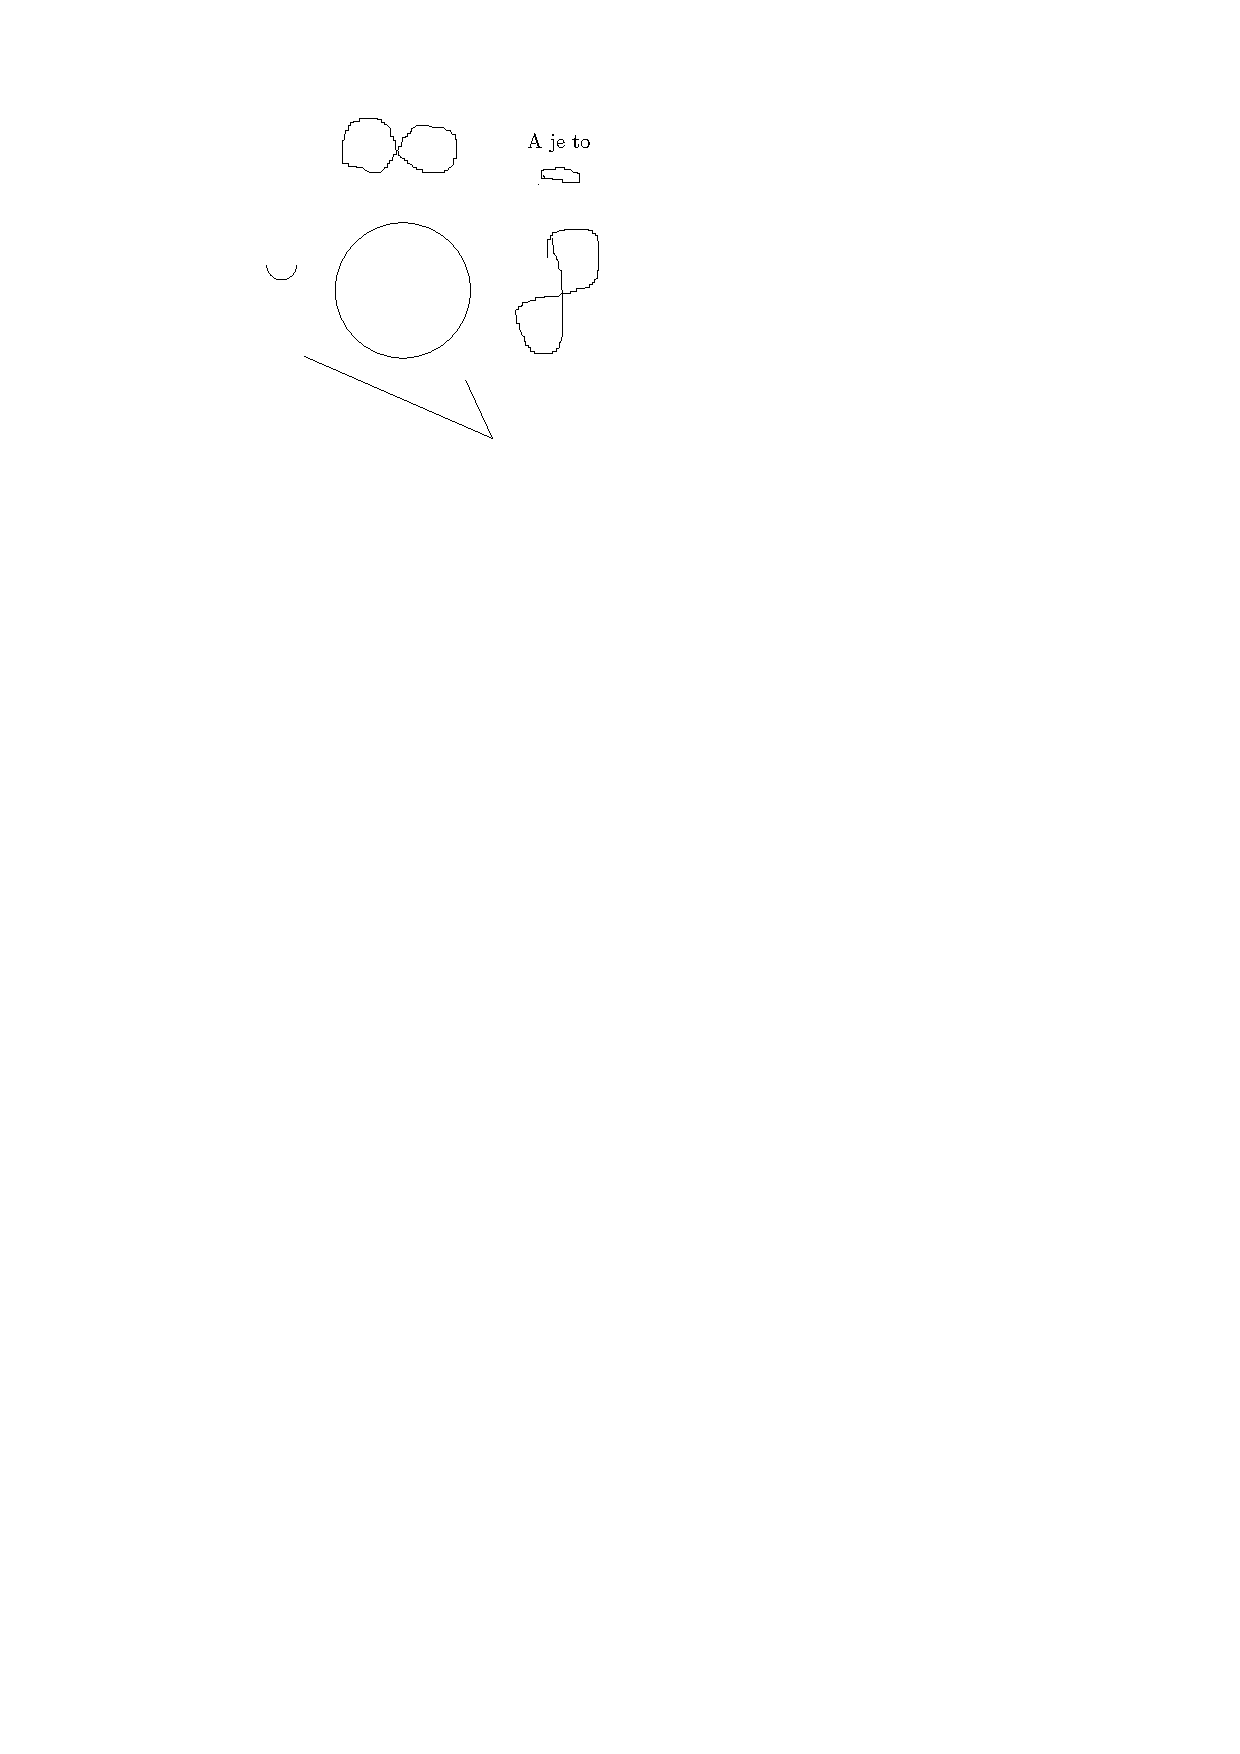
\includegraphics{Obrzkusmo.pdf}
\caption{Obrázek v pdf kreslený v ipe} %popisek obrázku automaticky doplněný o číslo a promítající se v seznamu obrázků
\end{center}
\end{figure}
\vspace*{10mm}
\begin{figure}[h] %obrázek musí být v plovoucím objektu figure; pro zabránění nežádoucího plavání po stránce se musí doplnit parametr "[h]"
\begin{center}

\includegraphics[width=15cm]{58.jpg} %příkaz width zmenší délku na zadaný rozměr fyzického papíru a zachová proporce
\caption{Fotka v jpg} %popisek obrázku automaticky doplněný o číslo a promítající se v seznamu obrázků
\end{center}
\end{figure}


%%Stránka pro zkoušení vkládání tabulek%%
\subsection{Vkládání tabulek}
Zkušební tvorba tabulek. Nejhorší je tvorba sirotků. Otázkou je, jak jím předejít. Klasické parametry nepomáhají. Problém se ani na fórech neřeší\ldots
\begin{table}[h] %tabulka "tabular" musí být uzavřena v plovoucím objektu "table"
\caption{Tabulka s přizpůsobením šířky sloupců}
\begin{center} %pro zarovnání tabulky na střed
\begin{tabular}{|l|c|c|} %zarovnání sloupců |left|center|center| oddělené čárou
\hline %horní horizontální čára
\textbf{Frekvenční pásmo} & \textbf{Technologie} & \textbf{Region} \\ %první řádka
\hline %oddělovací čára
700Mhz & LTE & USA \\ %druhá řádka 
\hline %oddělovací čára
800Mhz & LTE & Evropa \\ %třetí řádka
\hline %oddělovací čára
850Mhz & GSM & USA \\ %čtvrtá řádka
\hline 
900Mhz & GSM & Evropa \\ 
\hline
1700Mhz & 3G & USA \\ 
\hline
1800Mhz & GSM & Evropa \\ 
\hline
1900Mhz & GSM & USA \\ 
\hline 
2100Mhz & 3G & Evropa \\ 
\hline
2600Mhz & LTE & Evropa \\ 
\hline
\end{tabular}
\end{center}
\end{table} 

Fixní šířka sloupce může být nastavena příkazem "p\{5cm\}", ale tento příkaz vynutí zarovnání doleva. Při požadavku na zarovnání na střed nebo doprava ho nelze použít a buňka se musí manuálně roztáhnout doplněním násilných mezer "~" v první řádce tak, aby všechny sloupce byly stejně široké.

\begin{table}[h] %tabulka "tabular" musí být uzavřena v plovoucím objektu "table"
\caption{Tabulka s fixní šířkou sloupců}
%fixní šířka sloupce může být nastavena příkazem "p{5cm}", ale tento příkaz vynutí zarovnání doleva, při požadavku na zarovnání na střed nebo doprava ho nelze použít a buňka se musí manuálně roztáhnout doplněním násilných mezer "~" v první řádce tak, aby všechny sloupce byly stejně široké
\begin{center} %pro zarovnání tabulky na střed
\begin{tabular}{|l|c|c|} %zarovnání sloupců |left|center|center| oddělené čárou
\hline %horní horizontální čára
\textbf{Frekvenční pásmo} & \textbf{~~~Technologie~~~} & \textbf{~~~~~~Region~~~~~~} \\ %první řádka doplněná násilnými mezerami "~" pro rotažení buněk, aby sloupce byly stejně široké
\hline %oddělovací čára
700Mhz & LTE & USA \\ %druhá řádka 
\hline %oddělovací čára
800Mhz & LTE & Evropa \\ %třetí řádka
\hline %oddělovací čára
850Mhz & GSM & USA \\ %čtvrtá řádka
\hline 
900Mhz & GSM & Evropa \\ 
\hline
1700Mhz & 3G & USA \\ 
\hline
1800Mhz & GSM & Evropa \\ 
\hline
1900Mhz & GSM & USA \\ 
\hline 
2100Mhz & 3G & Evropa \\ 
\hline
2600Mhz & LTE & Evropa \\ 
\hline
\end{tabular}
\end{center}
\end{table} 


%%Stránka pro zkušební sazbu rovnic"
\subsection{Sazba rovnic}
Slavná rovnice Alberta Einsteina praví: $E = m \cdot c^2$. Platí pro všechny částice s nenulovou klidovou hmotností. Energie fotonu je naproti tomu determinována pouze jeho frekvencí (a Planckovou konstantou) $E = h * f$.
%sazba rovnice přímo v textu se provádí mezi dvěma znaky "$...$"

Nyní se podíváme na zoubek číslovaným rovnicím. Co třeba takhle první Maxwellova rovnice v diferenciálním tvaru?
\begin{equation} \label{max1} %číslovaná rovnice mimo text se uvádní příkazem "equation"; příkaz "label" slouží pro vytvoření návěští pro hypertextový odkaz na rovnici
\rot\vec{H}=\vec{J}+\dfrac{\partial \vec{D}}{\partial t}
%"\rot" - rotace; "\vec" - znak vektoru; "\frac{}{}" - rovnice; "\partial" - znak diferenciální rovnice 
\end{equation}

Pro sazbu matematiky platí obecně jiná pravidla. Jinak se například zadávají mezery nebo tučné písmo.
\begin{equation}
\forall x \in \mathbf{R}: \qquad x^{2+p} \geq 0
%"\forall" - znak "pro všechna"; "\in" - znak "je prvkem"; "\mathbf{}" - tučné písmo v rovnici; "\qquad" - delší mezera v rovnici; více znaků v jednom místě musí být uzavřeno mezi "{}"; "\geq" - znak "větší nebo rovno"
%pro tučné nevzpřímené symboly je místo "\mathbf{}" nutno použít "\boldsymbol"
\end{equation}

Zkusíme i odkazování. Vzpomínáte si na první Maxwellovu rovnici? Jestli ne, je to tato: \ref{max1}. Btw., znáte ten hezký symbol pro množinu reálných čísel? Je to tento: $\mathbb{R}$
%"\ref{max1}" - slouží pro vytvoření hypertextového číslovaného odkazu na rovnici (návěští max1)
%"\mathbb{R}" - vloží prokládaný znak R

A teď třeba funkce a odmocniny. Jako příklad do písemky z matematiky. Najděte definiční obor funkce:
\begin{equation}
f(x):\quad\left(\dfrac{\sqrt{3^{-x}}}{\sqrt[3]{x-7}}\right)^2
%"\quad" - mezera; "\left(" - levá závorka přes celou výšku následujícího výrazu (zlomku); "\dfrac" - zlomek; "\sqrt[3]" - 3. odmocnina; "\rigt)" - uzavření závorky přes celou výšku výrazu 
\end{equation} 

Studenti, pamatujete si ještě, derivace? Tohle musíte umět z hlavy i kdybych vás probudil uprostřed noci: $y=\cos(x^3)\qquad y'= \qquad y''=$
%"'" popř. "''" - první popř. druhá derivace

Kdo z vás si vzpomene ještě na limity a ví, co tato znamená?
\begin{displaymath}
\lim_{x \rightarrow 0} \frac{\sin x}{x} = 1
%limita odkud kam se zadává jako dolní index: "lim_{x \rightarrow 0}"; "\rightarrow" - šipka doprava používaná v limitě; "\sin" - sin a další se zadávají přes lomítko, aby byly vzpřímeným písmem
\end{displaymath}

Vrátíme se zpět k Maxwellovým rovnicím. Budeme pokračovat popořadě a podíváme se na druhou Maxwellovu rovnici, tentokrát v integrálním tvaru:
\begin{equation}
\oint_c \vec{E} \overrightarrow{\ud l} = -\frac{\ud\Phi}{\ud t}
%"\oint_c" - křivkový integrál po křivce c (zadává se jako dolní index); "\overrightarrow{} - šipka vektoru ale přes více znaků; "\ud" - vzpřímené "d" používané v integrálu; "\Phi" - velké řecké fí 
\end{equation}

A nyní něco trochu komplikovanějšího. Jak se spočte taková zřídlovost?
\begin{equation}
\nabla \times \vec{E} = \rot \vec{E} = \left| 
%"\nabla" - nabla; "\times" - vektorové "krát"; "\rot" - rotace; "\left|" - závorky determinantu
\begin{array}{c c c}
%determinant nebo matice se zadávají přes prostředí "array", parametry udávají počet sloupců a jejich centrování ("c" - na střed)
\vec{i} & \vec{j} & \vec{k} \\
%zadávání jako u tabulky: "&" pro další buňku, "\\" pro další řádek
\frac{\partial}{\partial x} & \frac{\partial}{\partial y} & \frac{\partial}{\partial z} \\
E_x & E_y & E_z
\end{array} \right|
\end{equation}

Občas bude zapotřebí vysázet víc rovnic současně. Například všechny Maxwellovy rovnice. Následující ukázka předvádí použití příkazu "align" nahrazující "equation" pro sazbu více rovnic. Rovnítko se musí doplnit znaky "\&": "\&=", aby byly rovnice správně vycentrovány na střed.
\begin{subequations}
%prostředí subequations zajistí podčíslování rovnic jako a, b, c
\begin{align}
%prostředí "align" nahrazuje "equation" pro sazbu více rovnic
f(x)&=\cos x
%rovnítko se musí doplnit znakem "&": "&=", aby byly rovnice správně vycentrovány na střed
\\
f'(x)&=-\sin x
\\
\udiv x &= 0
%pro divergenci se musí použít "\udiv" namísto "\div"
\end{align}
\end{subequations}

\noindent
%"\noindent" - zajistí, že následující odstavec na začátku nebude odsazený
Nebo napsat vysvětlivku k rovnici, která nebude odsazená.


%Zkušební stránka odrážek a číslování%%
\subsection{Odrážky a číslování}

\subsubsection{Odrážkovaný seznam}
Státy USA, které jsem navštívil:
\begin{itemize}
%prostředí "itemize" vytvoří zařážkový seznam; příkaz "\item[-]" může být doplněn "-" pro nahrazení koleček pomlčkami
\item Kalifornie
%příkazem "\item" se přidávají jednotlivé položky
\item Florida
\item New Jersey
\item New York
\item Illinois
\item Wisconsin
\item Minnesota
\item Pensylvánie
\item Maryland
\item Virginia
\item District of Columbia
\end{itemize}

\subsubsection{Číslovaný seznam}
Pořadí, v jakém jsem je navštívil:
\begin{enumerate}
%prostředí "enumerate" vytvoří číslovaný seznam
\item Illinois
%příkazem "\item" se přidávají jednotlivé položky
\item Wisconsin
\item Minnesota
\item Kalifornie
\item New York
\item New Jersey
\item Pensylvánie
\item Maryland
\item District of Columbia
\item Virginia
\item Florida
\end{enumerate}

\subsubsection{Popisné výčty (prostředí ,,Description'')}
Hlavní města některých států USA, které jsem navštívil:
\begin{description}
%prostředí description vytvoří seznam, kde je první část (název) zvýrazněno, za ním následuje text
\item[Kalifornie] Sacramento
%příkazem "\item[]" se přidávají jednotlivé položky, do "[]" se uvede název (to co bude tučně)
\item[Wisconsin] Madison
\item[Maryland] Annapolis
\end{description}

\subsubsection{Odsazování - tabulátor}
Největší města některých států USA, která jsem navštívil:
\begin{tabbing} %začátek odsazovaného prostředí tabulátoru
\hspace{5cm}\=\kill %parametrem v "\hspace{cm}" je délka odsazení tabulátoru
Illinois \> Chicago \\ %nejdříve první část, potom tabulátor "\>" a druhá část
Maryland \> Baltimore \\ 
Kalifornie \> Los Angeles 
\end{tabbing} 

\subsection{Citace}
\LaTeX ~nabízí i speciální prostředí pro citace a zvýraznění textu:
\begin{quote} %začátek prostředí pro citaci
\emph{,,Veni, vidi, vici.''} %zvýraznění (kurzíva) citace 
\end{quote}

\subsection{Verbatim}
Prostředí ,,Verbatim'' se hodí na sazbu textů, kde není žádoucí brát zřetel na formátovací značky. Příkladem je sazba zdrojových kodů.
%začátek prostředí verbatim pro sazbu bez ohledu na formátovací značky
\begin{verbatim}
System.out.println("Ja su lama, nevzpomenu si ani na zapis hlavicky v Jave")
\end{verbatim}


%%Závěr%%
\clearpage %\newpage nefunguje, po plouvocím objektu (obrázek, tabulka) musí pro novou stránku následovat "clearpage" 
\section{Závěr}
Věřím, že se povede dojít až k úspěšnému odvození finálních rovnic a vytvoření modulu pro modelování vysokofrekvenčního pole.

V současné době zdokonaluji kapitolu o vlnovodech a chtěl bych odvodit okrajové podmínky pro Helmholtzovu rovnici (ale nevím, co to je ani jak na to) - samotnou Helmholtzovu rovnici jsem již odvodil. Také bych Helmholtzovu rovnici chtěl vyjádřit ve válcových souřadnicích.

V další fázi bych dotáhl do konce kapitolu o šíření vln ve volném prostoru a vytvořil kapitolu (nebo přílohu) se stručnými informacemi o programu Agros2D a jeho ovládání.

Poté přijde na řadu to nejtěžší. Zjistit bližší informace o tom, co jsou to tzv. slabé formy, odvodit rovnice, vytvořit modul a analyzovat jeho chování uvnitř programu Agros2D.

Na závěr potom porovnat jeho chování a modelování vysokofrekvenčních zařízení v programu Comsol.

Modleme se za to, že se práce úspěšně povede dotáhnout do konce a v dubnu tady bude moci čnít: ,,Práce dokončena''

In nomine Patris et Filii et Spiritus Sancti. Amen.

%%Použitá literatura%%
\newpage
\phantomsection %Pro správné zobrazení čísla stránky v pdf rejsříku a přesný hyperodkaz
\addcontentsline{toc}{section}{Použitá literatura}
\begin{thebibliography}{10}

%Do "{}" příjmení autora, za to vložit z citace.cz, na název kurzívu
%Podle názvu v "{}" se poté odkazuje uvnitř textu pomocí příkazu "\cite{}" 
\bibitem{Pozar2} POZAR, David M. \textit{Microwave Engineering}. John Wiley \& Sons, Inc., 1998. Second Edition. ISBN 0-471-17096-8.
\bibitem{Pozar4} POZAR, David M. \textit{Microwave Engineering}. John Wiley \& Sons, Inc., 2012. Fourth Edition. ISBN 978-0-470-63155-3.
\bibitem{Kastner} KASTNER, Raphael. SCHOOL OF ELECTRICAL ENGINEERING, Tel Aviv University. Antennas and Radiation. Tel Aviv, 2009. Dostupné z: http://www.scribd.com/doc/56316827/3/Maxwell-Equations-in-the-Frequency-Domain
\bibitem{Dimensions} Rectangular waveguide dimensions. Microwaves101.com [online]. Tucson, AZ, November 3, 2012 [cit. 2012-11-19]. Dostupné z: http://www.microwaves101.com/encyclopedia/waveguidedimensions.cfm
\bibitem{Microstrip} Microstrip. Microwaves101.com [online]. Tucson, AZ, February 18, 2012 [cit. 2012-11-19]. Dostupné z: http://www.microwaves101.com/encyclopedia/microstrip.cfm
\bibitem{Instrinsic} Intrinsic Impedance. Antenna-Theory.com [online]. (c) 2009-2011 [cit. 2012-11-19]. Dostupné z: http://www.antenna-theory.com/definitions/intrinsicimpedance.php
\bibitem{Agros} KARBAN, Pavel. FACULTY OF ELECTRICAL ENGINEERING, University of West Bohemia in Pilsen. Agros2D [online]. Plzeň, 2012 [cit. 2012-11-19]. Dostupné z: http://www.agros2d.org/
\bibitem{Koudela} KOUDELA, Lukáš. \textit{Simulace šíření elektromagnetických vln.} Plzeň, 2011. Diplomová práce. Západočeská univerzita v Plzni, Fakulta elektrotechnická, Katedra teoretické elektrotechniky. Vedoucí práce Ing. Pavel Karban, Ph.D.
\bibitem{RovinnaVlna} Rovinné vlny. \textit{Fyzikální sekce Matematicko-fyzikální fakulty UK} [online]. [cit. 2013-02-20]. Dostupné z: http://physics.mff.cuni.cz/kfpp/skripta/kurz\_fyziky\_pro\_DS/display.php/optika/1\_3
\bibitem{hpFEM} THE HP-FEM GROUP. \textit{www.hpFEM.org} [online]. 2013 [cit. 2013-04-09]. Dostupné z: http://hpfem.org/


\end{thebibliography}

%%Seznam obrázků%%
\newpage
\phantomsection %Pro správné zobrazení čísla stránky v pdf rejsříku a přesný hyperodkaz
\addcontentsline{toc}{section}{Seznam obrázků}
\setlength{\parskip}{0ex}%Aby nebyly moc velké mezery mezi řádky seznamu obrázků a tabulek
\listoffigures

%%Seznam tabulek%%
\newpage
\phantomsection %Pro správné zobrazení čísla stránky v pdf rejsříku a přesný hyperodkaz
\addcontentsline{toc}{section}{Seznam tabulek}
\listoftables

%%Přílohy%%
\newpage
\pagestyle{empty} %vypnutí číslování
\setcounter{page}{1} %číslo stránky nastaveno na "1"
\appendix %deklarace, že se jedná o přílohu
\phantomsection %Pro správné zobrazení čísla stránky v pdf rejsříku a přesný hyperodkaz
\addcontentsline{toc}{section}{Přílohy}
\section*{Příloha I. - XML kód pro TE}
\subsection*{Zápis slabých formulací fázoru~E}
\label{xmlE}
\begin{spverbatim}
  <module:volume>
    <module:quantity id="rf_te_permittivity" shortname="rf_eps"/>
    <module:quantity id="rf_te_permeability" shortname="rf_mur"/>
    <module:quantity id="rf_te_conductivity" shortname="rf_gamma"/>
    <module:quantity id="rf_te_current_density_external_real" shortname="rf_Jer"/>
    <module:quantity id="rf_te_current_density_external_imag" shortname="rf_Jei"/>
    <module:weakforms_volume>
      <module:weakform_volume analysistype="harmonic" equation="\curl \left( \frac{1}{\mu}\, \curl \vecfaz{E} \right) - \mj \omega \left( \sigma + \mj \omega \varepsilon \right) \vecfaz{E} = \mj \omega \vecfaz{J}_{\mathrm{ext}}">
        <module:quantity id="rf_te_permittivity"/>
        <module:quantity id="rf_te_permeability"/>
        <module:quantity id="rf_te_conductivity"/>
        <module:quantity id="rf_te_current_density_external_real"/>
        <module:quantity id="rf_te_current_density_external_imag"/>
        <module:matrix_form axi_linear="- 1 / (rf_mur * MU0) * (r * udr * vdr + r * udz * vdz + (r > 0) * uval * vval/r + uval * vdr + vval * udr) + r * pow(2 * PI * f, 2) * rf_eps * EPS0 * uval * vval" axi_newton="- r * 1 / (rf_mur * MU0) * (udr * vdr + udz * vdz) + r * pow(2 * PI * f, 2) * rf_eps * EPS0 * uval * vval" i="1" id="form" j="1" planar_linear="- 1 / (rf_mur * MU0) * (udx * vdx + udy * vdy) + pow(2 * PI * f, 2) * rf_eps * EPS0 * uval * vval" planar_newton="- 1 / (rf_mur * MU0) * (udx * vdx + udy * vdy) + pow(2 * PI * f, 2) * rf_eps * EPS0 * uval * vval" symmetric="0"/>
        <module:matrix_form axi_linear="- 1 / (rf_mur * MU0) * (r * udr * vdr + r * udz * vdz + (r > 0) * uval * vval/r + uval * vdr + vval * udr) + r * pow(2 * PI * f, 2) * rf_eps * EPS0 * uval * vval" axi_newton="- r * 1 / (rf_mur * MU0) * (udr * vdr + udz * vdz) + r * pow(2 * PI * f, 2) * rf_eps * EPS0 * uval * vval" i="2" id="form" j="2" planar_linear="- 1 / (rf_mur * MU0) * (udx * vdx + udy * vdy) + pow(2 * PI * f, 2) * rf_eps * EPS0 * uval * vval" planar_newton="- 1 / (rf_mur * MU0) * (udx * vdx + udy * vdy) + pow(2 * PI * f, 2) * rf_eps * EPS0 * uval * vval" symmetric="0"/>
        <module:matrix_form axi_linear="2 * PI * f * rf_gamma * uval * vval" axi_newton="0" i="1" id="form" j="2" planar_linear="2 * PI * f * rf_gamma * uval * vval" planar_newton="0"/>
        <module:matrix_form axi_linear="-2 * PI * f * rf_gamma * uval * vval" axi_newton="0" i="2" id="form" j="1" planar_linear="- 2 * PI * f * rf_gamma * uval * vval" planar_newton="0"/>
        <module:vector_form axi_linear="- r * 2 * PI * f * rf_Jei * vval" axi_newton="- 1 / (rf_mur * MU0) * (updr * vdr + updz * vdz) + r * pow(2 * PI * f, 2) * rf_eps * EPS0 * upval * vval - r * rf_Jer * vval" i="1" id="form" j="1" planar_linear="- 2 * PI * f * rf_Jei * vval" planar_newton="- 1 / (rf_mur * MU0) * (updx * vdx + updy * vdy) + pow(2 * PI * f, 2) * rf_eps * EPS0 * upval * vval - rf_Jer * vval"/>
        <module:vector_form axi_linear="r * 2 * PI * f * rf_Jer * vval" axi_newton="- 1 / (rf_mur * MU0) * (updr * vdr + updz * vdz) + r * pow(2 * PI * f, 2) * rf_eps * EPS0 * upval * vval - r * rf_Jei * vval" i="2" id="form" j="2" planar_linear="2 * PI * f * rf_Jer * vval" planar_newton="- 1 / (rf_mur * MU0) * (updx * vdx + updy * vdy) + pow(2 * PI * f, 2) * rf_eps * EPS0 * upval * vval - rf_Jei * vval"/>
      </module:weakform_volume>
    </module:weakforms_volume>
  </module:volume>
\end{spverbatim}


\subsection*{Zápis okrajových podmínek fázoru~E}
\label{xmlEs}

\begin{spverbatim}
 <module:surface>
    <module:quantity id="rf_te_electric_field_real" shortname="rf_Er"/>
    <module:quantity id="rf_te_electric_field_imag" shortname="rf_Ei"/>
    <module:quantity id="rf_te_magnetic_field_real" shortname="rf_Hr"/>
    <module:quantity id="rf_te_magnetic_field_imag" shortname="rf_Hi"/>
    <module:quantity id="rf_te_surface_current_real" shortname="rf_Jr"/>
    <module:quantity id="rf_te_surface_current_imag" shortname="rf_Ji"/>
    <module:quantity id="rf_te_impedance" shortname="rf_Z0"/>
    <module:weakforms_surface>
      <module:weakform_surface analysistype="harmonic" default="rf_te_electric_field">
        <module:boundary equation="\vecfaz{E} = \vecfaz{E}_0" id="rf_te_electric_field" name="Electric field">
          <module:quantity id="rf_te_electric_field_real"/>
          <module:quantity id="rf_te_electric_field_imag"/>
          <module:essential_form axi_linear="rf_Er" axi_newton="rf_Er" i="1" id="form" planar_linear="rf_Er" planar_newton="rf_Er"/>
          <module:essential_form axi_linear="rf_Ei" axi_newton="rf_Ei" i="2" id="form" planar_linear="rf_Ei" planar_newton="rf_Ei"/>
        </module:boundary>
        <module:boundary equation="n \times H = n \times H_0" id="rf_te_magnetic_field" name="Magnetic field">
          <module:quantity id="rf_te_magnetic_field_real"/>
          <module:quantity id="rf_te_magnetic_field_imag"/>
          <module:vector_form axi_linear="r * 2 * PI * f * rf_Hi * vval" axi_newton="r * 2 * PI * f * rf_Hi * vval" i="1" id="form" j="1" planar_linear="2 * PI * f * rf_Hi * vval" planar_newton="2 * PI * f * rf_Hi * vval"/>
          <module:vector_form axi_linear="- r * 2 * PI * f * rf_Hr * vval" axi_newton="- r * 2 * PI * f * rf_Hr * vval" i="2" id="form" j="2" planar_linear="- 2 * PI * f * rf_Hr * vval" planar_newton="- 2 * PI * f * rf_Hr * vval"/>
        </module:boundary>
        <module:boundary equation="\faz{J}_{t} = - \frac{1}{\omega \mu} \frac{\partial \vecfaz{E}}{\partial n_0} = \faz{J}_0" id="rf_te_surface_current" name="Surface current">
          <module:quantity id="rf_te_surface_current_real"/>
          <module:quantity id="rf_te_surface_current_imag"/>
          <module:vector_form axi_linear="- 2 * PI * f * rf_Ji * r * vval" axi_newton="- 2 * PI * f * rf_Ji * r * vval" i="1" id="form" j="1" planar_linear="- 2 * PI * f * rf_Ji * vval" planar_newton="- 2 * PI * f * rf_Ji * vval"/>
          <module:vector_form axi_linear="2 * PI * f * rf_Jr * r * vval" axi_newton="2 * PI * f * rf_Jr * r * vval" i="2" id="form" j="2" planar_linear="2 * PI * f * rf_Jr * vval" planar_newton="2 * PI * f * rf_Jr * vval"/>
        </module:boundary>
        <module:boundary equation="- \frac{1}{\omega \mu} \frac{\partial \vecfaz{E}}{\partial n_0} = \sqrt{\frac{\varepsilon - \mj \sigma / \omega}{\mu}} \vecfaz{E}" id="rf_te_impedance" name="Impedance boundary condition">
          <module:quantity id="rf_te_impedance"/>
          <module:matrix_form axi_linear="r * 2 * PI * f / rf_Z0 * uval * vval" axi_newton="-r * 2 * PI * f / rf_Z0 * uval * vval" i="1" id="form" j="2" planar_linear="2 * PI * f / rf_Z0 * uval * vval" planar_newton="- 2 * PI * f / rf_Z0 * uval * vval"/>
          <module:matrix_form axi_linear="- r * 2 * PI * f / rf_Z0 * uval * vval" axi_newton="r * 2 * PI * f / rf_Z0 * uval * vval" i="2" id="form" j="1" planar_linear="- 2 * PI * f / rf_Z0 * uval * vval" planar_newton="2 * PI * f / rf_Z0 * uval * vval"/>
          <module:vector_form axi_linear="0" axi_newton="r * 2 * PI * f / rf_Z0 * upval * vval" i="1" id="form" j="1" planar_linear="0" planar_newton="2 * PI * f / rf_Z0 * upval * vval"/>
          <module:vector_form axi_linear="0" axi_newton="r * 2 * PI * f / rf_Z0 * upval * vval" i="2" id="form" j="2" planar_linear="0" planar_newton="2 * PI * f / rf_Z0 * upval * vval"/>
        </module:boundary>
      </module:weakform_surface>
    </module:weakforms_surface>
  </module:surface>
\end{spverbatim}


\newpage
\section*{Příloha II. - XML kód pro TM}
\subsection*{Zápis slabých formulací fázoru~H}
\label{xmlH}

\begin{spverbatim}
<module:volume>
    <module:quantity id="rf_tm_permittivity" shortname="rf_eps"/>
    <module:quantity id="rf_tm_permeability" shortname="rf_mur"/>
    <module:quantity id="rf_tm_conductivity" shortname="rf_gamma"/>
    <module:quantity id="rf_tm_current_density_external_real" shortname="rf_Jer"/>
    <module:quantity id="rf_tm_current_density_external_imag" shortname="rf_Jei"/>
    <module:weakforms_volume>
      <module:weakform_volume analysistype="harmonic" equation="\curl \left( \frac{1}{\mu}\, \curl \vecfaz{H} \right) - \mj \omega \left( \sigma + \mj \omega \varepsilon \right) \vecfaz{H} = - \curl \vecfaz{J}_{\mathrm{ext}}">
        <module:quantity id="rf_tm_permittivity"/>
        <module:quantity id="rf_tm_permeability"/>
        <module:quantity id="rf_tm_conductivity"/>
        <module:quantity id="rf_tm_current_density_external_real"/>
        <module:quantity id="rf_tm_current_density_external_imag"/>
        <module:matrix_form id="form" axi_linear="- r * 1 / (rf_eps * EPS0) * (udr * vdr + udz * vdz) + r * pow(2 * PI * f, 2) * rf_mur * MU0 * uval * vval" axi_newton="0" i="1" j="1" planar_linear="- 1 / (rf_eps * EPS0) * (udx * vdx + udy * vdy) + pow(2 * PI * f, 2) * rf_mur * MU0 * uval * vval" planar_newton="0" symmetric="0"/>
        <module:matrix_form id="form" axi_linear="- r * 1 / (rf_eps * EPS0) * (udr * vdr + udz * vdz) + r * pow(2 * PI * f, 2) * rf_mur * MU0 * uval * vval" axi_newton="0" i="2" j="2" planar_linear="- 1 / (rf_eps * EPS0) * (udx * vdx + udy * vdy) + pow(2 * PI * f, 2) * rf_mur * MU0 * uval * vval" planar_newton="0" symmetric="0"/>
        <module:matrix_form id="form" axi_linear="r * 2 * PI * f * rf_gamma * 1 / (rf_eps * EPS0) * uval * vval" axi_newton="0" i="1" j="2" planar_linear="2 * PI * f * rf_gamma * 1 / (rf_eps * EPS0) * uval * vval" planar_newton="0"/>
        <module:matrix_form id="form" axi_linear="- r * 2 * PI * f * rf_gamma * 1 / (rf_eps * EPS0) * uval * vval" axi_newton="0" i="2" j="1" planar_linear="- 2 * PI * f * rf_gamma * 1 / (rf_eps * EPS0) * uval * vval" planar_newton="0"/>
        <module:vector_form id="form" axi_linear="0" axi_newton="0" i="1" j="1" planar_linear="0" planar_newton="0"/>
        <module:vector_form id="form" axi_linear="0" axi_newton="0" i="2" j="2" planar_linear="0" planar_newton="0"/>
     </module:weakform_volume>
    </module:weakforms_volume>
  </module:volume>
\end{spverbatim}


\subsection*{Zápis okrajových podmínek fázoru~H}
\label{xmlHs}

\begin{spverbatim}
 <module:surface>
    <module:quantity id="rf_tm_electric_field_real" shortname="rf_Er"/>
    <module:quantity id="rf_tm_electric_field_imag" shortname="rf_Ei"/>
    <module:quantity id="rf_tm_magnetic_field_real" shortname="rf_Hr"/>
    <module:quantity id="rf_tm_magnetic_field_imag" shortname="rf_Hi"/>
    <module:quantity id="rf_tm_surface_current_real" shortname="rf_Jr"/>
    <module:quantity id="rf_tm_surface_current_imag" shortname="rf_Ji"/>
    <module:quantity id="rf_tm_impedance" shortname="rf_Z0"/>
    <module:weakforms_surface>
      <module:weakform_surface analysistype="harmonic" default="rf_tm_magnetic_field">
        <module:boundary equation="\vecfaz{H} = \vecfaz{H}_0" id="rf_tm_magnetic_field" name="Magnetic field">
          <module:quantity id="rf_tm_magnetic_field_real"/>
          <module:quantity id="rf_tm_magnetic_field_imag"/>
          <module:essential_form id="form" axi_linear="rf_Hr" axi_newton="0" i="1" planar_linear="rf_Hr" planar_newton="0"/>
          <module:essential_form id="form" axi_linear="rf_Hi" axi_newton="0" i="2" planar_linear="rf_Hi" planar_newton="0"/>
        </module:boundary>
        <module:boundary equation="n \times E = n \times E_0" id="rf_tm_electric_field" name="Electric field">
          <module:quantity id="rf_tm_electric_field_real"/>
          <module:quantity id="rf_tm_electric_field_imag"/>
          <module:vector_form id="form" axi_linear="- 2 * PI * f * rf_Ei * r * vval" axi_newton="0" i="1" j="1" planar_linear="- 2 * PI * f * rf_Ei * vval" planar_newton="0"/>
          <module:vector_form id="form" axi_linear="2 * PI * f * rf_Er * r * vval" axi_newton="0" i="2" j="2" planar_linear="2 * PI * f * rf_Er * vval" planar_newton="0"/>
        </module:boundary>
        <module:boundary equation="\faz{J}_{t} = - \frac{1}{\omega \mu} \frac{\partial \vecfaz{E}}{\partial n_0} = \faz{J}_0" id="rf_tm_surface_current" name="Surface current">
          <module:quantity id="rf_tm_surface_current_real"/>
          <module:quantity id="rf_tm_surface_current_imag"/>
          <module:vector_form axi_linear="- 2 * PI * f * rf_Ji * r * vval" axi_newton="0" i="1" id="form" j="1" planar_linear="- 2 * PI * f * rf_Ji * vval" planar_newton="0"/>
          <module:vector_form axi_linear="2 * PI * f * rf_Jr * r * vval" axi_newton="0" i="2" id="form" j="2" planar_linear="2 * PI * f * rf_Jr * vval" planar_newton="0"/>
        </module:boundary>
        <module:boundary equation="- \frac{1}{\omega \mu} \frac{\partial \vecfaz{E}}{\partial n_0} = \sqrt{\frac{\varepsilon - \mj \sigma / \omega}{\mu}} \vecfaz{E}" id="rf_tm_impedance" name="Impedance boundary condition">
          <module:quantity id="rf_tm_impedance"/>
          <module:matrix_form axi_linear="r * 2 * PI * f / rf_Z0 * uval * vval" axi_newton="0" i="1" id="form" j="2" planar_linear="- 2 * PI * f * rf_Z0 / uval * vval" planar_newton="0"/>
          <module:matrix_form axi_linear="- r * 2 * PI * f / rf_Z0 * uval * vval" axi_newton="0" i="2" id="form" j="1" planar_linear="2 * PI * f * rf_Z0 / uval * vval" planar_newton="0"/>
          <module:vector_form axi_linear="0" axi_newton="0" i="1" id="form" j="1" planar_linear="0" planar_newton="0"/>
          <module:vector_form axi_linear="0" axi_newton="0" i="2" id="form" j="2" planar_linear="0" planar_newton="0"/>
        </module:boundary>
      </module:weakform_surface>
    </module:weakforms_surface>
  </module:surface>
\end{spverbatim}


\end{document}
